 %	Skriv folgende ind som en custom Quick Build (F1)
%pdflatex -interaction=nonstopmode %.tex|bibtex %|pdflatex -interaction=nonstopmode %.tex|pdflatex -interaction=nonstopmode %.tex

\documentclass[english,twoside,openright]{report}

\usepackage[utf8]{inputenc}
\usepackage[T1]{fontenc} 
\usepackage{babel}

\usepackage{xcolor}% provides \colorlet
\usepackage{fixme}
\fxsetup{
    status=draft,
    author=,
    layout=inline,
    theme=color
}

\definecolor{fxnote}{rgb}{0.8000,0.0000,0.0000}
% define the background colour:
\colorlet{fxnotebg}{yellow}
\definecolor{fxfatalbg}{rgb}{0,0,100}

% refedine the layout macro:
\makeatletter
\renewcommand*\FXLayoutInline[3]{%
  \@fxdocolon {#3}{%
    \@fxuseface {inline}%
    \colorbox{fx#1bg}{\color {fx#1}\ignorespaces #3\@fxcolon #2}}}
\makeatother

\usepackage{rotating}

\usepackage{graphicx}
\usepackage{wrapfig}
\usepackage{appendix}
\usepackage{float}
\usepackage{lipsum}
\usepackage{lastpage}
\usepackage{fancyhdr}
\usepackage{varioref}
\usepackage{hyperref}    % Creates links in the PDF
\usepackage{listings}
%\usepackage{algorithmic}
\usepackage{listings}
\usepackage{tabularx}
\usepackage{subfig} %til resize af billeder
%\usepackage[usenames,dvipsnames]{color}
\definecolor{lightgray}{RGB}{232,232,232}
\usepackage{spverbatim} %Bruges til at indføre wrapping i kodemiljøer, ellers er den magen til {verbatim}
\usepackage{bussproofs} %Bruges til at indf�re derivationstr�er
\usepackage[ final ]{pdfpages}
\usepackage{epstopdf}
\usepackage[section]{placeins}

%Acronymer for P6 Giraf Projekt
\newcommand{\secref}[1]{Section \ref{#1}}
\usepackage{acronym}
\acrodef{api}[API]{Application Programming Interface}
\acrodef{cat}[CAT]{Category Administration Tool}
\acrodef{lamp}[LAMP]{Linux, Apache2, MySql and PHP}
\acrodef{giraf}[GIRAF]{Graphical Interface Resources for Autistic Folk}
\acrodef{oha}[OHA]{Open Handset Alliance}
\acrodef{gui}[GUI]{Graphical User Interface}
\acrodef{json}[JSON]{JavaScript Object Notation}
\acrodef{foss}[FOSS]{Free and Open-Source Software}

\lstdefinelanguage{cs}
  {morekeywords={abstract,event,new,struct,as,explicit,null,switch
		base,extern,object,this,bool,false,operator,throw,
		break,finally,out,true,byte,fixed,override,try,
		case,float,params,typeof,catch,for,private,uint,
		char,foreach,protected,ulong,checked,goto,public,unchecked,
		class,if,readonly,unsafe,const,implicit,ref,ushort,
		continue,in,return,using,decimal,int,sbyte,virtual,
		default,interface,sealed,volatile,delegate,internal,short,void,
		do,is,sizeof,while,double,lock,stackalloc,
		else,long,static,enum,namespace,string,MySQLTools,MySqlDataAdapter },
	  sensitive=false,
	  morecomment=[l]{//},
	  morecomment=[s]{/*}{*/},
	  morestring=[b]",
}

\lstdefinelanguage{nisse}
     {morekeywords={title,subtitle,url,@begin,@end,@setting,@u,@b,@i,@apply,@image,@title,@subtitle,@note,fade,swipe,scale,rotatescale,global,text,image,@url,@font_family,@font_color,@font_size,@font_weight},
	  sensitive=true,
}


% CODE %
\usepackage{listings}
\usepackage{color}
\usepackage{textcomp}
\definecolor{listinggray}{gray}{0.9}
\definecolor{lbcolor}{rgb}{0.9,0.9,0.9}
\lstset{
	language=nisse,
	keywordstyle=\bfseries\ttfamily\color[rgb]{0,0,1},
	identifierstyle=\ttfamily,
	commentstyle=\color[rgb]{0.133,0.545,0.133},
	stringstyle=\ttfamily\color[rgb]{0.627,0.126,0.941},
	showstringspaces=false,
	basicstyle=\small,
	numberstyle=\footnotesize,
	numbers=left,
	stepnumber=1,
	numbersep=10pt,
	tabsize=2,
	breaklines=true,
	prebreak = \raisebox{0ex}[0ex][0ex]{\ensuremath{\hookleftarrow}},
	breakatwhitespace=false,
	aboveskip={1.5\baselineskip},
  	columns=fixed,
  	upquote=true,
 	extendedchars=true,
escapeinside={(*@}{@*)},         % if you want to add a comment within your code
}


% Bibtex %
\usepackage{natbib}

% URL %
\usepackage{url}
\makeatletter
\def\url@leostyle{\@ifundefined{selectfont}{\def\UrlFont{\sf}}{\def\UrlFont{\small\ttfamily}}}
\makeatother
\urlstyle{leo}


\setlength{\headheight}{15pt}
\pagestyle{fancy}
\renewcommand{\chaptermark}[1]{\markboth{#1}{}}
\renewcommand{\sectionmark}[1]{\markright{#1}{}}
 
 
\fancyhf{} % clear header and footer
\fancyhead[LO, RE]{\textit{\rightmark}}
\fancyhead[RO, LE]{\textit{\leftmark}}


\fancypagestyle{plain}{
\fancyhead[LE,RO,RE,LO]{}
\renewcommand{\headrulewidth}{0pt}
\fancyfoot[RO,LE]{\thepage\ of \pageref{LastPage}}}
\fancyfoot[RO,LE]{\thepage\ of \pageref{LastPage}}
\newenvironment{boenumerate}
  {\begin{enumerate}\renewcommand\labelenumi{\textbf\theenumi}}
  {\end{enumerate}}

\begin{document}
	
	\lstset{frameround=tttt, escapeinside={\%}{\%}}
	
	%\title{GIRAF - Admin}
%\author{By: Group SW601F12}
%\date{\emph{May 2013}}
%\maketitle
%\newpage

\thispagestyle{empty}
\begin{flushright}
\vspace{3cm}

\phantom{hul}

\phantom{hul}

\phantom{hul}

\textsl{\Huge GIRAF - Admin} \\ \vspace{1cm}

\rule{13cm}{3mm} \\ \vspace{1.5cm}
\vspace{1cm}


\includegraphics[width=0.75\textwidth]{images/girafAdminLogo.png}

\vspace{1.5cm} 
\textsc{\Large SW6 Projekt \\
Group SW601F13 \\
Department of Computer Science\\
Aalborg University\\
June 4$^{th}$ 2013\\}
\end{flushright}

	\addtocounter{page}{1}
	\newpage
%\addtocounter{page}{1}
\thispagestyle{empty}
\mbox{}
%	\setcounter{page}{2}
	\thispagestyle{empty}
\begin{titlepage}
	\addcontentsline{toc}{chapter}{Title Page}
	\setcounter{page}{3}
\begin{nopagebreak}
{\samepage 
\begin{tabular}{r}
\parbox{\textwidth}{  \raisebox{-14mm} {
\includegraphics[height=3.0cm]{images/aau-stud-logo.pdf}}
\hfill \parbox{4.9cm}{\begin{tabular}{l}
{\sf\small \textbf{Department of Computer Science}}\\
{\sf\small  \textbf{Aalborg University}} \\
{\sf\small Selma Lagerl\"{o}fs Vej 300} \\
{\sf\small Telephone: +45 9940 9940} \\
{\sf\small Telefax:   +45 9940 9798} \\
{\sf\small http://cs.aau.dk}
\end{tabular}}}
\\
\end{tabular}
\vspace{-12pt}
\begin{tabular}{cc}
\parbox{7cm}{
\begin{description}

\item {\bf Title:} 

GIRAF - Admin

\item {\bf Theme:} 

Developing Complex Software Systems

\end{description}

\parbox{8cm}{

\begin{description}
\item {\bf Project period:}\\
   P6, Spring Term 2013\\
  \hspace{4cm}
\item {\bf Project group:}\\
  SW601F13\\
  \hspace{4cm}
\item {\bf Participants:}\\
Jens M. Lauridsen\\
Johan Sørensen \\
Lars Chr. Pedersen\\
Tommy Knudsen
  \hspace{2cm}
\item {\bf Supervisor:}\\
Shuo Shang
\end{description}
}
\begin{description}
\item {\bf Circulation:} 7
\item {\bf Page count:} \pageref{LastPage}
\item {\bf Appendix count and type:} 5, Installation Guide and Configuration, Graphical Mockups of the GIRAF System,  Transcript of Meeting with the head of kindergarten (1/3 2013), Usability Testing Appendix, Colour Theme
\item {\bf Finished on} June 4$^{th}$ 2012
\end{description}
\vfill } &
\parbox{7cm}{
  \vspace{.15cm}
  \hfill 
  \begin{tabular}{l}
  {\bf Synopsis:}\bigskip \\
  \fbox{
    \parbox{6.5cm}{\bigskip
     {\vfill{\small This report documents the development of an administration system for the GIRAF system as of Software 6 multiproject 2013. The administration system is designed for high maintainability and user friendliness. The back-end for the system is written entirely in PHP, the front-end is a combination of HTML, JavaScript and CSS. The administration system should enable users to administrate users, applications and pictgrams. However the pictogram and application systems are not fully implemented. To administrate pictograms refer to the Parrot project under the GIRAF system. Mockups of the complete system is viewable in the appendix.
     \bigskip}}
     }}
   \end{tabular}}
\end{tabular}}
\\ \\ \\ \\
\noindent{\footnotesize\emph{The report content is freely available, but publication (with source), only after agreement with the authors.}}
\end{nopagebreak}
\end{titlepage}
	\newpage
%\addtocounter{page}{1}
\thispagestyle{empty}
\mbox{}
	\chapter*{Preface}
\label{chap:preface}
This report is written by four students from the Department of Computer Science at Aalborg University, and is part of the multi project GIRAF. The four students are studying as Software Engineers at their 6th semester.\\
\\
This report both serves as a documentation of the project process as well as documentation of how the system works.\\
\\
Included with this report, there is a CD containing the projects Git repository. Which contains the report, source code of the system as well as the graphic assets used in the project.\\
\\
The group would like to personally thank:\\
Ulrik Nyman for great input and support during the project.\\
Mette Als for her patience and valuable input into the designing of the system.\\

	\newpage
%\addtocounter{page}{1}
\thispagestyle{empty}
\mbox{}
%	\setcounter{page}{4}
	\chapter*{Signatures:}
	\addcontentsline{toc}{chapter}{Signatures}

\noindent\rule{8cm}{0.03cm}\\
Tommy Knudsen\\

\noindent\rule{8cm}{0.03cm}\\ 
Lars Chr. Pedersen\\ 

\noindent\rule{8cm}{0.03cm}\\
Johan Sørensen\\

\noindent\rule{8cm}{0.03cm}\\
Jens Mikkel Lauridsen\\

	\newpage
%\addtocounter{page}{1}
\thispagestyle{empty}
\mbox{}
%	\setcounter{page}{6}
	\tableofcontents	
	\addcontentsline{toc}{chapter}{Contents}
	\newpage
	\section{Danish mini report}
Projektet Admin er et underproject af GIRAF sytemet der har været under udvikling siden 2011. Admin har til fokus at udvikle administrations interface til GIRAF systemet til håndtering af bruger, pictogramer og applikationer.\\
For forårssemesteret 2013 havde Admin projektet fokus på at omdesign interfaceet til et et system der er nemmer at vedligeholde på tablet og desktop samt mere brugervenligt.\\
For at skabe et projekt der samtidig også er optimal at arbejde videre på årene der kommer er først fokus at få indentifiseret alle funtionaliteter der er krav på og designede dette i et samhængende system.\\
Hovedfunktionaliteten der skulle være funtionel efter projektet afslutning ved sommeren 2013 er bruger håndtering.   
Bruger håndtering er vigtigst da det er dette der gør hele GIRAF systemet brugbart for børn og pædagorer. \\

Problemfoumulering for projektet var: 
\begin{verse}
\textit{``Currently there are two different administration interfaces for the GIRAF system.
This results in a problem with maintainability and user friendliness.
How can we make a \underline{single} user friendly administration interface for the GIRAF system?''}
\end{verse}

og på dansk: 
\begin{verse}
\textit{``På nuværende tidspunkt er der to forskellige adminstrations interface for GIRAF systemet.
Dette speber problemer med vedligeholdelse og brugervenlighed. 
Hvordan er det multigt at skabe et \underline{enkelt} brugervenligt adminstrations interface for GIRAF systemet?''}
\end{verse}


Systemet er bygget i PHP,  og Apache. Målet med projektet var også at lave et system som både kunne køre på en PC, men også på en Android tablet. Et forslag på en løsning er at bruge PAW, som gør det muligt at eksekverer PHP på en Android tablet. \\ \\
En stor del af fokusen i projektet har også været at gøre det så nemt som muligt for den gruppe som tager over, at fortsætte med projektet. Rapporten består af flere dele der beskriver projektets udvikling. Delene består af et login system, et profil system, et pics (billede) system, et QR kode system og et app system. \\ \\
Designet af systemet er bygget ovenpå Twitters Bootstrap, som hjælper med hurtigt at udvikle hjemmesider. Det overordnet design er baseret på GIRAF design guidelines. Login systemet er opbygget ved hjælp af PHPs session. Der er også udviklet et multi-sprog system som er bygget til at efterligne Android's sprog system. Dette gør at det er nemt at tilføje nye sprog til systemet, samt at folk som er bekendt med Android's system hurtigt vil blive bekendt med systemet. Pics systemet er lavet sådan at man nemt fra sin PC kan tilføje nye pics til systemet, samt tilknytte pics til et barn, da det tidligere har været svært at tilføje allerede eksiterende pics til GIRAF systemet. QR kode systemet er lavet til at hvis man taber sin QR kode, så er det muligt at få lavet en ny. QR kode systemet bruger et bibliotek kaldet phpqrcode, som gør det muligt at tage en tekststreng og lave det til et billede som viser QR koden. App systemet er designet sådan at man kan bestemme hvilke apps et barn har mulighed for at gå ind i. \\ \\
Under projektet er der desuden lavet en brugervenlighedstest, hvor testpersoner blev inviteret til at afprøvet systemet. Ved hjælp af brugervenlighedstesten blev der fundet en del fejl og mangler, hvor nogle af dem nåede at blive rettet. På grund af problemer med en anden gruppe nåede alle funktioner i systemet ikke at blive færdig, og disse er beskrevet i rapporten. \\
For at konkludere så er projektet ikke færdigt, men der er sat et godt grundlag for den næste gruppe der skal arbejde videre med projektet. Yderligere er der også givet forslag til hvad den næste gruppe kan lave videre på, for at gøre systemet bedre.
	\chapter*{Introduction}
This project is part of the multi-project called GIRAF, which stands for: ''Graphical Interface Resources for Autistic Folk'' which have been an active project at Aalborg University since 2011.\\
As the name suggests this system is a tool made for helping kids with autism to communicate. The system is to be actively used in the specialized kinder gardens and schools here in Aalborg.\\
This report contains first an introduction to the GIRAF project as a whole, which describes the GIRAF project as it is of the day this report was written. This introduction is contained in all project reports for the GIRAF multi-project, and can therefore be skipped if the reader already is familiar with the GIRAF project as of year May 2013. The place to be skipped to is then part \vref{skipToMe}.\\
Second this report also contains the thoughts that went into constructing the new administration system, as well as some in depth going explanation of the implementations, for the GIRAF system.\\
The administration system makes it possible to edit and create users for the GIRAF system and in its finished form is possible to be controlled both from a tablet and from a PC over the internet. It also comes with the possibility to make, edit and manage pictograms on a PC over the internet.\\
\\
In this report we also use some terms that often is misunderstood, as well as a few special words, we therefore want to clarify them here before we begin. The wording is taken from wikipedia \citep{wikipedia}.


\begin{table}[h]
	\centering
		\begin{tabular}{|l|l|}
			\hline
			Word & Meaning\\\hline\hline
			Website & A set of related webpages served from a single web domain\\\hline
			Webpage & A single page displayed on a website\\\hline
			Homepage & The initial or main web page of a website\\\hline
			Site & Refers to the word website\\\hline
			Pictogram & A special element, developed for the GIRAF project. Containing sound, text and image\\\hline
			Guardian & A person with responsibility for a child with autism, either a pedagog or a parent\\\hline
		\end{tabular}
	\caption{Word Explanation}
	\label{tab:WordExplanation}
\end{table}

	\newpage
%\addtocounter{page}{1}
\thispagestyle{empty}
\mbox{}
	\part{GIRAF Introduction} %Put it in if needed

\chapter{The GIRAF Project}

\ac{giraf} started in 2011 as a semester project targeting children with autism and their guardians. %Allthough solutions exists these were expensive and did not provide the needed level of user-customization\todo{Er dette virkelig korrekt?}.
 In the following chapter, the overall vision for the \ac{giraf} project will be presented, the projects from previous years will be explained briefly along with the platform for the project. Lastly a section describing autism is included.


%% \todo{Write a little section about the contents of this chapter.}

%% \todo{Figure out which order this should be in}

\section{Vision for \acs{giraf}}
The vision for \ac{giraf} is to create a multi-purpose application based on \emph{Android} which can simplify and ease the lives of autistic children and their guardians.

The purpose of \ac{giraf} is to replace physical items that are being used daily by the children and their guardians with digitized versions. The idea is to gather several functionalities in one object and allowing customization for each individual child.

This will also optimize work procedures on the individual institution in such a way, that guardians will save time doing repetitive tasks such as making pictograms. This time could be spent with the children instead.

As of spring of 2013 three schools and institutions for children with autism in Northern Jutland are involved in the development, but the hope is that \ac{giraf} will be distributed across all similar institutions in Denmark.


\section{Previous Years}
%This section briefly describes the projects developed for the \ac{giraf} project during 2011 and 2012.

During the first year of development, four parts of the \ac{giraf} project were developed. The four projects were developed during the spring semester of 2011 and included the projects:
\begin{description}
\item [Admin] An administration interface used for administrating different aspects of the \ac{giraf} system.
\item [DigiPECS] A digitized version of ``Picture Exchange Communication System''\cite{pecs} a system used as an aid for communication with people with special needs such as autism.
\item [Launcher] A home screen application and distribution platform for Android.
\item [aSchedule] A visual schedule for the Android platform.
\end{description}

During the spring semester of 2012, five new software groups continued development of the \ac{giraf} project. The projects developed during 2012 were:

\begin{description}
\item [Launcher] An enhancement of the launcher project developed during the spring semester of 2011.
\item [Oasis] An enhancement of the admin project from 2011. Furthermore the Oasis project developed a local database for the \ac{giraf} system.
\item [Parrot] An enhancement of the DigiPECS project from 2011. The project was renamed because of trademark issues.
\item [Savannah] A server side database with web interface for the \ac{giraf} system.
\item [Wombat] An Android application for measuring and visualizing time.
\end{description}

%During the spring semester of 2012, two different projects working with databases were developed although the databases from the two projects were never made able to synchronize.
During the spring semester of 2012 two databases were developed, however synchronization between them was never achieved.

\subsection*{Problems with Initial Implementation}
As the spring semester of 2013 started, an ''install party'' for the students was held. The party was intended to help the students compile and deploy the projects from 2012.

Even though a representative for each of the 2012 groups were present, some compilation problems still occurred.

The repository used for distributing in 2012, was disorganized and difficult to navigate, i.e. due to:
\begin{itemize}
  \item Multiple copies of the same project.
  \item Unclear dependencies among the different projects.
  \item Projects only meant to be compiled from Eclipse for Windows.
\end{itemize}

During the following week a working workspace was created and shared with the rest of the students, along with install instructions. The install instructions were later updated to a more clear edition.


\section{Target Platform}
\label{sec:platform}
Android is an open-source operating system originally developed by Android Inc, and later bought by Google Inc. The first release came in 2007, where it was launched by Google Inc. together with \ac{oha}, which includes companies such as Samsung, HTC, LG and Google.

Before the first students where involved in the project in the spring of 2011 Ulrik Nyman considered two platforms for the development of the project. The Android and iOS platforms. The Android platform was chosen for three main reasons:
\begin{itemize}
\item That the platform is open source.
\item That in Android the developers can take control of the functionality of the home button.
\item That distribution of the software is possible outside the official marketplace.
\end{itemize}

For the two following years it has been chosen to stay on the Android platform. This is done to be able to both reuse the source code and because Android compatible hardware is available for the students.
In the very long term the system could support multiple platforms.

%Android was chosen as the target platform because it is open-source.
%The following years it was chosen to continue the work from previous rather than to start from scratch by choosing a different platform, and the development platform is therefore still Android.

%% The previous projects used Android as the development platform, which is also the reason why Android was picked for this semester project. Alternative platforms could be iOS or the newly released Windows 8. If one of these was chosen, the project would have to start from scratch.

%The Android \ac{api} allows for easy development e.g. to gain access to the device's camera, microphone etc. thus allowing to use the inputs gained from these in an easy way.


\section{Autism}
\label{sec:autism}
Autism is a spectrum disorder, meaning that it appears in different variants and not all people who are diagnosed have the same symptoms. The disorder can often be observed within the first three years of a child's life.
Autism is a physical condition and is linked to abnormal chemistry in the brain, however the exact causes of these abnormalities are still unknown.\citep{autism}

%In general autism appears in three different variants. These are different diagnosis of autism:

%% It affects the development of some parts of the brain, especially areas concerned with social and communication skills. Autism affect how information is processed in the brain by altering how the brain's nerve cells and synapses connect. How this is occurs is not very well understood,\citep{autism} and due to this there is not existing cure for autism.

%\begin{description}
%\item [ADHD] Attention Deficit/Hyperactivity Disorder
%\item [Tourette] Verbal and motor tics
%\item [Chromosomal defects] \todo{THere is still missing something here}
%\end{description}


\subsection*{Symptoms}
\label{sub:symptoms}
Children with autism usually have difficulties understanding the concept of ``play pretend'', meaning that they have a hard time imitating the actions of others when playing and therefore prefer to play alone. Furthermore they have difficulties with social interaction and communication -- verbally and non-verbally.

People diagnosed with autism may;

%% Every person with autism is different, just like normal people, however in general people with autism may:

\begin{itemize}
\item Be very sensitive to light, noise, touch, and taste.
\item Have a hard time adjusting to new and changing routines.
\item Show unusual attachments to objects.
\end{itemize}

Autism diagnosed individuals may have a hard time starting and maintaining a conversation. They may communicate with gestures instead of words, develop language slower or faster than normal and some do not develop any language at all.
Furthermore the lack of social interaction means they might have a hard time making friends, may be withdrawn and may avoid eye contact.\citep{autism}

\subsection*{Signs and tests}
\label{sub:signsAndTests}
If a child fails to meet any of the following language milestones, it may be an indication that it needs to be tested for autism;

\begin{itemize}
\item Babbling by 12 months.
\item Gesturing (such as pointing or waving goodbye) by 12 months.
\item Saying single words by 16 months.
\end{itemize}

Children failing to meet any of the previous mentioned language milestones might receive a hearing evaluation, a blood test and a screening test for autism. Since autism covers a broad spectrum of symptoms, a single brief evaluation cannot predict what abilities the child has. Therefore a range of different skills are evaluated, such as:

\begin{itemize}
\item Communication
\item Language
\item Motor skills
\item Speech
\item Success at school
\item Thinking abilities
\end{itemize}

Some parents might be scared of having their child diagnosed, %because they are scared of labelling what is wrong with their child,
however without a diagnosis, the child might not get the necessary help.\citep{autism}

\subsection*{Treatment}
\label{sub:treatment}
Autism cannot be cured, however an early diagnosis and treatment can greatly improve the child's quality of life. Different treatment programs usually build on the child's interests and are highly structured to their needs and routines.\citep{autism}


\chapter{The GIRAF Project 2013}

When working in a multi-project consisting of eight groups, it is important to have a common goal for the project. This chapter describes this goal as a story. Furthermore the chapter includes description of the development process and the rules of conduct.  %as well as the rules of conduct, that was used in the \ac{giraf} project of year 2013.

\section{The Goals for 2013}
Within the first couple of weeks, when all the groups had been assigned a project, a major story for the overall project was written.

\subsection*{The Major Story for 2013}
\begin{quote}
``The guardian arrives at the institution, and turns on the tablet. The guardian is aware of the arrival of a new child at the institution after lunch.
The guardian sets up and customizes a profile for the child, this includes creation of new pictograms. Furthermore the guardian prepares games and a life story for the child.

After lunch the new child and the guardian meet. The child is introduced to the communication tool Parrot. After some introduction they sit down to do some communication practice using the tool.

Afterwards the child wants to go outside to see the rest of the institution, and needs to put on some outdoor clothes. The guardian introduces the child to the Zebra tool, and together they put on the child's outdoor clothes.

When the child comes back in, the guardian and the child play the games prepared earlier by the guardian.

When they are done playing the child and the guardian read the child's life story using Tortoise.''
\end{quote}


%% \todo{Write a little section about the contents of this chapter}

% \section{How do we work}

% % File for section about the major story for this year

\section{The goal for 2013}

\subsection{The major story for 2013}
\begin{quote}
"The guardian arrives at the institution, and turns on the tablet.
The guardian knows that a new child is to arrive at the institution
after lunch. The guardian sets up and customizes a profile for the child,
this include creations of new pictograms.
The guardian also prepares games and a lifestory for the child.

After lunch the new child and the guardian meet, they immediately sit
down to do some communication practice using Parrot.

Afterwards the child wants to go outside to see the rest of the
institution, and needs to put on some outdoor clothes. The guardian
introduces the child to Zebra, and together they put on the child's
outdoor clothes.

When the child comes back in, the guardian and the child play the games
prepared earlier by the guardian.

When they are done playing the child and the guardian read the child's
lifestory using Tortoise."
\end{quote}


\section{Definition of a Multi-Project}
\label{sec:multiproject}
A multi-project is a project which includes multiple groups which each work on their own sub-project, which is part of a larger project. In this case, the larger project is the \ac{giraf} system and each group works on a separate part of the system.

Compared to working on a single project in isolation, working together creates new challenges. The software produced by each group has to be integrated to ensure the entire system works properly. Some projects are more independent on the rest, while others depends heavily on some projects like the database project Wasteland described in \secref{sub:wasteland}. Groups have to be flexible and pass any requirements to other groups' projects early to prevent halts.

To ensure the project is successful and no misunderstandings occur, there must be good communication and cooperation between the groups. This requirement is amplified by the fact that there are no definitive authoritative figures, other than those chosen by project members.


\section{Group and Work Structure}
%% This section describes bla bla bla \todo{Write the intro}
%% This section includes a description of the development methods and tools implemented during the spring semester of 2013.
%% The section includes a description of the development methods used during the spring semester of 2013,
This section describes the development methods used during the spring semester of 2013, including stories and project management tools.

The section is rounded off by a description of the development tools used, including Redmine, Git, and Jenkins.

\subsection{Development Method}
\label{sec:development}
Having a development method is one of the main ways to structure the work process of a project.
A development method is a collection of methods and structures, from the way to have meetings, gathering requirements and structuring the development.
There are many development methods, each is structured and handles issues differently,
%But talking about implementing a development method is often not a 1:1 implementation. Even though there exist many development methods,
however, it is rare that one fits a development problem perfectly.
Different methods are often combined and customized to fit the problem at hand.
%Therefore it is often the case, that different methods are merged together to structure a more specific method for a given project. For this project, most of the methods used come from the agile paradigm, which is an iterative development method.

\subsubsection{Implemented Development Methods}
\label{subsub:implementedDevelopmentMethods}
%This project with it's alteration of teams, working on, for many, new platform, team cooperation and focus on a finished product i all things that talk for at agile development.
This project's nature calls for agile development, due to team collaboration, user feedback, product focus, and continuous integration.
Agile development focuses on a flexible but structured work progress suited for projects with many unknown variables.
%Many agile development methods also focus on having a shippable product throughout the project period.
The agile development method has the ability to adapt to changing requirements throughout the project and focuses on having a shippable product at the end of each iteration. %secures a firm and safe development.

\subsubsection{Stories}
\label{subsub:stories}
%An agile develop method and a team structure with many team and few members with high interaction between team requires a high level of management.
%To ensure cooperation between teams and reaching deadlines with shippable products are many SCRUM method tools implemented.
User stories is one of the tools that helps streamline the work process, keeps focus on a shippable product and is the main component for management of the project. First of all the product story works as a common problem statement for all work groups. A product story is the agreement on what is necessary for the product to be finished. From product story each group can extract what is required of them to complete the story.

\subsubsection{Management}
\label{subsub:management}
The semester coordinator, Ulrik Nyman, has supervised the project since its beginning. Ulrik Nyman himself has a child with autism and will continue being a part of the project for the time to come, conveying his knowledge of the development process and the product.
%The product has focus on helping children with autism but mostly in a kindergarten in context with guardians.
%He does not have much/any expertise in this area therefore is a number of guardians used as clients/consultants to test and comment on the requirements and design of the product.
To help fit the product to the needs of guardians, for whom the product is intended, a number of representatives are included for more detailed feedback on the process and the product.

%A critical problem of a product story is to ensure that work is not forgotten or one assignment is made and specialized by more teams.

%SCRUM uses a product manager and SCRUM masters to ensure all requirements are met and any conflicts are resolved. %To extract one person for a team of four to function as SCRUM master is an inefficient solution.
%The SCRUM master uses most of his resources on gathering and transferring information leaving little to develop.
To keep as many work hours in development and to keep a good overall management, common meetings were held weekly.
The common meetings had focus on sprints and team cooperation. Problems that needed further discussion and/or development were discussed by a committee consisting of a few representatives from each group.

%The story committee is the main committee to make the SCRUM work.
%The story committee had a meeting at the end of each sprint, often 3-5 days before common meeting, where the next sprint story is discussed so each group is firm on their assignment for the sprint. Before the meeting is there feature freeze so the committee can discuss the former sprint without further development.
%In the feature freeze the teams is to write documentation of their sprint and assemble their product.
%Lastly the common meeting has the function of booting the next sprint to the groups at the common meeting.
The common meeting and committee meeting are further specified in sections \secref{sub:theweeklymeeting} and \secref{subsub:importantcommittees}.

\subsection{Development Tools}
\label{sub:devtools}
A number of tools were used in order to optimize team collaboration and to make the projects more accessible. These tools will be further explained in the following sections.

A dedicated Linux server was commissioned for the entire \ac{giraf} project and several services installed to facilitate collaboration and agile development. Common to all current services are their free, open-source nature and support of LDAP authentication, allowing all students and supervisors to log in using their AAU credentials.
%A number of tools are used to ensure a shippable product and a well documented work progress.
%For the tools and big solution agreed on, either from a common meeting or committee, is a person set as controller, maintainer or/and guide.
%This person is often are person that have a high knowledge level of the tool or was in close development of the solution.

\subsubsection{Redmine}
\label{subsub:redmine}
Several tools were audited for use in the project management aspect of development, including Trac, PivotalTracker and Github. Redmine, a Ruby-On-Rails web application, was selected owing primarily to its support of multiple projects and support features such as wikis, forums, milestones and various charts. The features most broadly used will briefly be described here.
% of the project was Redmine. Redmine includes many functions but only the ones used in the multi-project will be described.
%Redmine was chosen because of the ability to divide form to bottom.
\begin{description}
	\item[Projects] All projects live in a shared project space, and can be placed in a hierarchy under a super project. In this regard, the primary multi project served as the base of each of the eight groups' underlying projects.
	\item[Issue handling] Redmine's primary feature is its issue handling. Project members can create and react to issues within custom-defined domains. For \ac{giraf}, this was primarily development tasks, but could just as well be used for report-related tasks or general maintenance in an attempt to manage time usage.
	\item[Burndown Charts] Redmine does not have native support for burndowns, but does support it through a \ac{foss} third-party plugin. Burndowns are a visual aid of each subproject's progress throughout a sprint, giving quick summary of development speed and whether proactive action may need to be taken.
	\item[Milestones] A generic milestone feature in Redmine is Versions. Versions are simply markers with a set date, and can be open or closed for attachment of issues. The burndown plugin couples a version's end date with attached issues and their progress to generate the related charts.
	\item[Wiki] A per-project wiki module exists in Redmine. The basic wiki markup has been expanded to allow referencing of almost any other element in the project hierarchy, such as projects, issues, files and VCS revision.
\end{description}

Redmine has many more features not directly applied during this project period. However, many could be applied to create a more centralised and structured development experience in future projects. Examples include file and document hosting, advanced issue workflows, permission management and VCS integration. Future multiprojects may consider expanding into these fields if they feel proficient in Redmine's basic usage.

% Redmine arranges the multi-project in a hierarchy, ordered in terms of teams, sprints, and issues.
%The multi-project is levelled from the main project to teams, sprints and lastly issues.
%Each issue can be specified with description, estimated time, progress, and more. An issue can be assigned to a team member. This provides an overview of each team member's workload. A sprint consists of multiple issues that are presented in an issue table. %The issues can be unmanageable to estimate whether the sprint is on time.
%A burndown chart is a graphical representation of remaining work versus estimated time.
%A burndown chart visualizes the estimated need be done each day to reach the deadline, the current workload and with the current speed the sprint is estimated done.
%The burndown chart is a key tool to manage sprints. At the start of each sprint the workload is estimated, from the burndown chart one can assess whether the workload is too large or small for the sprint. %Through out the sprint can the estimated finish time with current work speed be analyzed against the needed work speed to meet the deadline.This can help correct the work progress before it is too late.
%A burndown chart can also be used on a higher level in the development hierarchy, providing an overview of the overall progress of the multi-project.
%The burndown chart is also implemented in the higher levels to keep the overview of each team and the overall project.
%Redmine also includes a wiki which is useful for gathering information in one place.

\subsubsection{Version Control System}
\label{subsub:git}
\label{subsub:vcs}
The university's IT services offers only a single version control system, Subversion. Although centrally supported and backed up regularly, Subversion's shortcomings were challenged before main development had begun. Most notably, the system's centralised workflow and high operation cost. Many of SVN's actions require access to the central server. Two alternatives without these issues were suggested: Git and Mercurial (Hg). The former was chosen as a general question of broad platform support and popularity. A primary strength of these systems is their support of separate branches of development without the constant need to connect to a central server. This allows developers of each project to synchronize with a main branch while maintaining several development branches on their own workstation.

Most groups used Github as hosting solution for development of their projects, as a git hosting solution was not immediately forthcoming (contrary to Subversion and Mercurial, Git does not have a default server implementation). At the conclusion of the project period, a solution was configured using Apache-based LDAP authentication, deferring authorisation and repository management to Gitolite, a low-footprint open-source offering.

In the interest of easier cross-project code contribution and inspection, an improved web solution may prove a better choice. Due to time constraints, a few solutions were briefly audited but ultimately discarded in preference of Gitolite. Gitlab should be mentioned as it featured an interface and features very close to those of Github itself, but proved difficult to install and maintain.

% Git was used for version control in the multi-project. Git benefits from being distributed which makes it possible for each developer to have personal branches, for working on features and bugs without have to synchronize with a central server.
  % Git is distributed version control solution, making the need for a central server non-critical. %% \todo{cite this}

\subsubsection{Jenkins}
\label{subsub:jenkins}
A principal element of agile development is continuous integration, the automated concurrent building of new code as it is pushed to central repositories which ensure constant availability of newest binary packages while catching coding errors before pushing them to the public. Jenkins, a fork of Oracle's Hudson, was suggested early and, given no proponents, was implemented. Build jobs were set up for each project, polling their origin repositories for new Git builds to main branches. If a repository has new code, it is downloaded and built. In case of build errors, the project developers are notified by email. To facilitate the deployment phase of each sprint, all projects are rebuilt every Thursday night and pushed to a public FTP server as well as making them publicly available by HTTP.

Git support is not part of Jenkins' core feature set, but is available as a plugin. During development, unhandled exceptions in the plugin code resulted in thousands of superfluous builds as a failed build due to unexpected circumstances was not marked as failed.

% Jenkins is a build script used to build all projects from the Git-hosting server, deploying a shippable product. If the build fails, the responsible individuals are notified of the situation so it can be corrected. Jenkins helps make sure that all sub-projects of the \ac{giraf} system can co-exist on the same platform and ``work together''.
%To secure the development of the project is the vision control system Git used.
%Git also support a multiple persons working same files or extract multiple branches to merge after.
%Git secures the all material can be restored if errors i committed with the vision control.
%With common base in Git is Jenkins use to assemble the project at the end of each week.
%This means that there is functional product each week and test each week of bugs and errors.

%\subsection{Project Development Overview}
%Using an agile development method helps structure the project with multiple to work in synchronization.
%Redmine is the management system to take advantage of the methods given by SCRUM.
%The work progress, issue management and information sharing is some of the key functions for Redmine.
%Git is the version control system that support different development methods for the preference of the team.
%A version control system of the product secures that errors not undermine the project.
%Jenkins assembles the project to a functional and shippable product each week.


\section{Decision Making - The Process}
\label{sec:decisionmaking}

The following section will describe the decision making process, set in place to ensure that everyone would be heard on an equal and democratic footing. The decision making process during this semester's multi-project consists of two different steps.

\subsection{The Weekly Meeting}
\label{sub:theweeklymeeting}

It was strongly recommended by the semester coordinator, Ulrik Nyman, to hold a weekly meeting for all software students on the bachelor semester of 2013. The meeting's agenda consists of a few points of formalism at the very beginning, in which a secretary and a moderator are chosen by means of voting. Candidates for these roles are entirely self-appointing and a vote is issued to pick one of the candidates. %and as such resolves any potential issues of personal discomfort (peer pressure or otherwise). A vote is then issued to pick one of the candidates.

Though the weekly meeting is established to ensure a higher level of communication between students, as well as to ensure that decisions will be taken on a multi-project level scale, not all points are actually discussed at this meeting. Instead, a committee approach is agreed upon, see \secref{sub:committees}. The purpose of establishing committees is to ensure that relevant discussions to a given topic can be had, but within a smaller audience.

Committees are discussed at the weekly meeting where voting determines which committees are established. A chairman for a committee is self-appointed and a vote determines if there is consent to let the given person be chairman.

The meeting will then proceed and discuss the ideas and suggestions agreed upon within each committee from the previous week and at the multi-project level determine, by voting, which ideas are okay, or if any of the points concluded by one of the committees are subpar and should be reworked.

\subsection{Rules of Conduct}
\label{sub:rulesofconduct}
During the first weekly meeting some general rules of conduct were established, including decisions on how voting should be done. A number of ways to do this were suggested. Ultimately it was decided that every person present at the meeting has an individual vote, and the idea of a group based voting system was therefore discarded. Furthermore in the event that there is a 50/50 split, the vote will have to be reissued. There must be majority 'for' or 'against' a decision. Guidelines for when a decision should be taken at the weekly meeting were established as well. If a decision involved only two or three groups, then it would not be necessary to discuss it at the weekly meeting. If, however, the decision impacted everyone, a committee would be established to make these decisions.

%Det er her jeg beskriver det med at modsætte sig en komit beslutning
%------------
%Decisions agreed upon in committees can be overruled by those attending the weekly meeting - however to disagree with a decision taken in a committee one has to write a letter for everyone to see explaining one's arguments. This letter must be accessible prior to attending a meeting so that everyone has a chance to read these arguments. %\todo{Blev det besluttet ? eller det mig der har d{\aa}rlig hukommelse?}
%------------

During a committee meeting every group has a single vote. It is possible to send as many group members as it is deemed necessary to the committee meetings, however, it does not increase the number of total votes a group has. %% Every group should keep in mind that the entire point of having committees is to reduce the amount of people attending a discussion significantly.

\subsection{Committees}
\label{sub:committees}
%A committee is established when the decision to be made within it requires consent from all or most groups, and it is deemed a too deep topic or challenging discussion to be discussed at a weekly meeting. This is typically because the decision(s) to be made, impacts everyone to some degree.
A committee ideally consists of a representative from each multi-project group and a chairman agreed upon at the weekly meeting. The chairman is responsible for setting up the meeting, time, place, agenda as well as writing down the details of what is agreed upon during the committee meeting. %The group representatives are responsible for attaining knowledge about the topic to be discussed to give a more educated opinion about the topic.
%This ensures that the weekly meeting stays an 'information-sharing' focused meeting whereas the committees will be in charge of making the tough decisions, that does not require consensus from every person participating in the multiproject.

The resulting work product of the committee is a document, that potentially answers every question on the agenda, ready to be presented at the next multi-project meeting.

\subsubsection*{Important Committees}
\label{subsub:importantcommittees}
The following section describes an extract of some of the most important committees, that were established during one of the first weekly meetings.

\begin{itemize}
        \item Wiki: \emph{Ensures that the multi-project wiki page on Redmine is created in a uniform way by establishing guidelines for new
        articles.}
        \item Design Guidelines: \emph{Ensures that the User Interface design of the \ac{giraf} application is uniform (e.g. in regards to font, color scheme and various buttons - green for `yes' and red for `no').}
        \item Common Report: \emph{This committee is responsible for the creation of the common-report chapters, which you are reading now, which are at the beginning of every semester report.}
        \item Pictogram Class: \emph{Because every group requires a common pictogram class, it was decided to create a Pictogram Class committee to determine the functionality that this class needed.}
        \item GIT: \emph{The GIT committee is responsible for working out a common structure across all repositories to create uniformity and make it easier to continuously integrate.}
        \item Public Pictogram: \emph{Determines guidelines for how pictograms are handled in the database (e.g. who has access rights to what and why?).}
        \item Story: \emph{The story committee is responsible for creating a story to follow every sprint. It puts the sprint's tasks into an overall context.}
        \item CI/Git: \emph{This committee is responsible for coming up with solutions to potential issues that might occur as part of the Continuous Integration step when using GIT.}
\end{itemize}


\chapter{What was developed}

%% This chapter presents the definition of a pictogram, and a description of the current use. Design guidelines for the whole application will be outlined together with digitizing and design of the pictograms.

%In this chapter the developed work of 2013 will be presented, this include description of the common done work the projects of 2013, and the chapter is rounded off by acknowledging the included people outside the projects groups.

This chapter describes the work done for \ac{giraf} in the year 2013 and is rounded off by acknowledging the involved contacts and the semester coordinator.

% \section{The common stuff}

\section{Pictograms, Morgana, and Design Guidelines}
In this section the notion of a pictogram will be presented followed by how pictograms are currently being used and why they should be digitized. Furthermore the section includes a description of the Morgana library.

The section will be rounded off with the overall design guidelines for the entire \ac{giraf} system.


\subsection{Pictogram}
\label{sub:pictogram}
%Intro
%What is a pictogram?
In the context of this report a pictogram is defined thus:
\emph{A pictogram is an image representing a living being, a physical object or some form of action.}
Pictograms can contain a text-label, describing the respective images, for clarification. There is currently no standard for the layout or contents of pictograms, due to the specific needs and opinions of the users. User \textbf{A} might like to have black and white images with text labels whereas user \textbf{B} might want colorful images without text. The images can themselves vary from cartoons to photographic representations.
Pictograms are commonly used as means of communication, especially by those requiring assistance with communicating, including but not limited to individuals with autism.

\subsubsection*{Current Use}
\label{subsub:pic_currentuse}
%How are they used today and what are their pros and cons.
%Give a quick description of the use in the facilities that we have visited.
\begin{figure}[!ht]
        \centering
        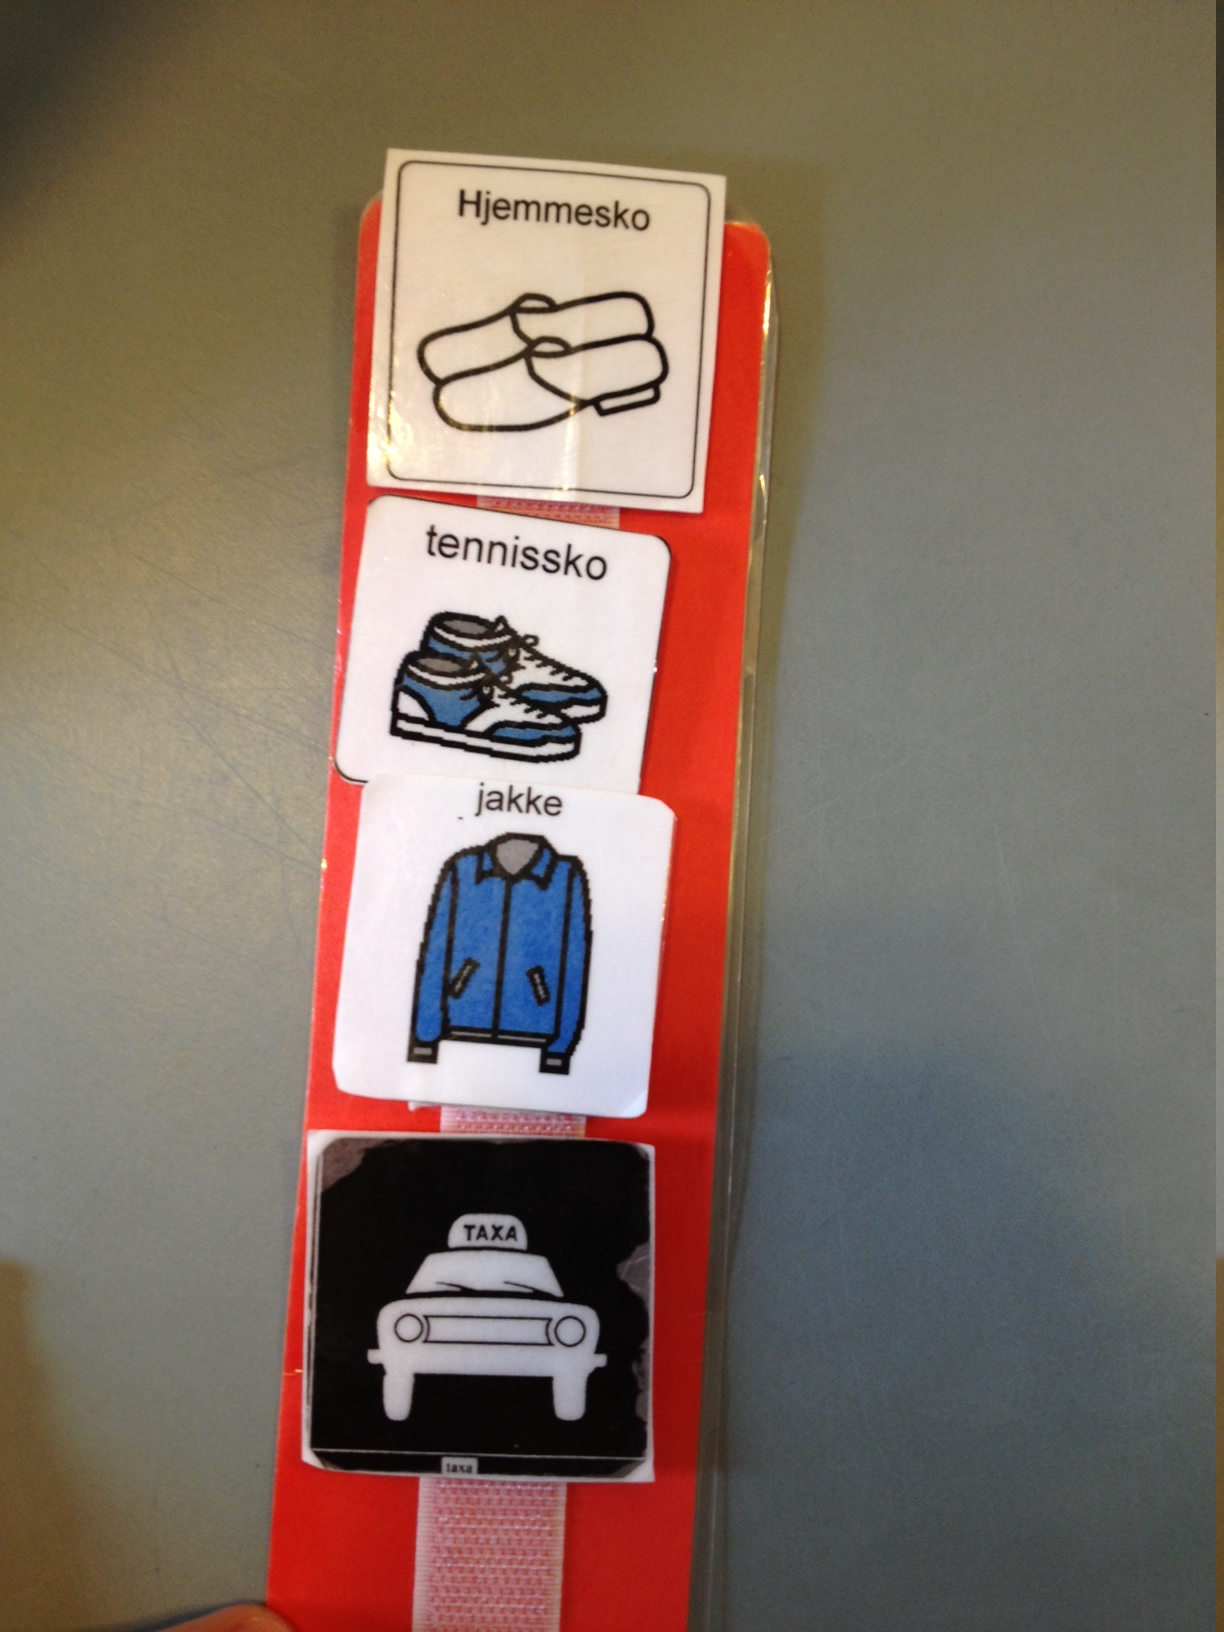
\includegraphics[scale=0.15]{cReport/img/current_use_picto.jpg}
        \caption{\label{img:pic_current} Pictograms in use 2013}
\end{figure}
During the spring semester of 2013, when this report was written, the use of pictograms is mostly in the form of physical images. The images need to be drawn and/or edited, printed, cut out and then laminated to extend their lifespan. After this process the pictograms are ready for use, generally for one individual, making this repetitive and tedious for the guardians.% \todo{Klim: Bliver dette virkelig kun brugt for et enkelt barn? Kan mapper ikke deles af flere b{\o}rn? Biggi: Nej det kan de ikke, det er blevet sagt af kontakt-person}
When the required amount of pictograms have been created for an individual, they need to be organized and made accessible with the help of some sort of container. This container can be a folder with a pocket for the pictograms and a velcro-like strip for arranging the pictograms. For communication an individual can choose to form sentences by arranging the pictograms accordingly or use a single image to simply express needs and wants. Another purpose of the pictograms can be to graphically represent instructions for various tasks, in the form of ``do \textbf{A}, followed by \textbf{B} and lastly do \textbf{C}'' for individuals requiring special assistance.

\subsubsection*{Digitizing the Pictogram}
%What's new, what had previous groups implemented, reflect on why it had to be redone.
The \ac{giraf} project focuses on simplifying and digitizing a medium used by individuals with autism and their guardians. This includes digitizing the pictograms, making them available on devices running Android with added functionality. Added functionality includes the option to make the pictograms play a sound, dynamically change the layout of text-labels and editing images. Digitizing the pictogram also makes it possible to share them easily, carry them between devices and make backups of them. Previously, with the same idea in mind, it was attempted to digitize the pictogram. It was considered unsatisfactory (see section below) and therefore the re-implementation in this semester's project.

\subsubsection*{GIRAF Pictogram Design}
%What is the pictogram (basically). What are the ideas behind the current design.
%How is this design better than the previous? How is it used?
The digitized pictogram consists of an image, a text-label and a sound. With all elements included, it can be presented as each of the three, two parts combined or all three in union. This viewable container is designed as an extension of the \emph{Android} view class, making it easy for developers to include and present in their applications. The idea is to have users sharing the same pictograms, with the option to customize their contents without affecting the pictogram itself. The previous \ac{giraf} pictogram design lacked documentation, portability and functionality such as text-labels. Therefore a new design was implemented, which hopefully fits the needs of both future \ac{giraf} developers and \ac{giraf} users.


\subsection{Morgana}
\label{sub:morgana:intro}
The Morgana library project was initially intended to make it possible for all the \ac{giraf} applications to use both the Wasteland database, see \secref{sub:wasteland}, and the local Oasis database seamlessly, however in the time allotted it was not possible to finish this functionality, so the focus was shifted to making it parse and write \ac{json} objects for use in calls to the Wasteland database.

The library implements a Java class for each value object documented in the Wasteland \ac{api}, each class parses a \ac{json} object and turns it into an object which can be used by \ac{giraf} applications, it is also able to create \ac{json} objects from the stored Java object.


\subsection{Design Guidelines}
\label{sub:designGuidelines}
The purpose with the guidelines is to get a consistent look and feel across all of the different applications included in the \ac{giraf} system.
The design guidelines have been discussed among all of the project groups, and they are as follows:

\begin{quote}
\begin{itemize}
\item Keep the existing color palette
\item Font: Helvetica
\item Font size: use common sense. \emph{Android} offers extra small/small/medium/large/huge
\item Minimize the use of text, use images instead of text
\item \ac{gui} in vector graphics
\item Green and red are universal colors for `accept'/`cancel'
\item Applications have animal icons
\item Icons are non-customizable
\item Every application should be locked in landscape mode
\end{itemize}
\end{quote}

The color palette will be the same as in the 2012 version of \ac{giraf}. With regards to font type and size, Helvetica has been chosen and developers need to keep in mind, that the text has to be readable on the tablet.

The aim is to use more images and less text as the target audience are mostly children, many of whom have communication and/or reading difficulties and some have problems imagining objects purely from text.

The \ac{gui} will be in vector graphics, because it scales well, which makes it possible to reuse some of the images. Green and red are universal colors for `accept'/`cancel'. It may sound obvious but other applications have been developed with different colors.
Tool-applications should have animal icons.

Lastly everything will be in landscape mode as this eliminates additional implementation for responsive layout, when the tablet is rotated.


\section{The Project of 2013}
\label{sec:projects}
\subsection{Admin}
\label{sec:admin}
This project focuses on the creation of an administration interface for the \ac{giraf} system. The Admin system consists of two parts, one for a desktop computer and one for \emph{Android}. The desktop part will run on a \ac{lamp} stack and communicate with the database using the database \ac{api} provided by the Wasteland (see \secref{sub:wasteland}) project. The \emph{Android} part will run on the tablet using the same code base as the desktop part, using a web server application. The main focus of the project is for department managers and guardians to be able to administrate the \ac{giraf} system.

\subsection{Cars}
\label{sub:cars}
The aim of the Cars project is to develop an application, which will help children with infantile autism to be more comfortable in using their voice. To ensure that the children learn how to use their voice in creating different types of sounds, and not just speak in a monotone way, the application will require the children to create sounds covering different sides of the frequency spectrum.

Cars is a game in which the player has to lead a car through a street into a garage, controlling it with high or low frequency sounds. The car has a matching coloured garage at the end, which when entered completes the game successfully.
%The car and garages are colored and the two need to match to successfully complete the game. 
Randomly placed obstacles are used to force the player to avoid them to reach the end.

\subsection{Croc}
\label{sub:Croc}

The Croc project aims to create an application for creation of pictograms for use in the \ac{giraf} system.

\begin{description}
\item  Pictograms can be created in a number of ways:
  \begin{description}
  \item[Camera] take a picture with the camera and turn that picture into a pictogram.
  \item[Drawing] draw a pictogram.
  \item[Audio] record sounds to attach to pictograms.
  \end{description}
\end{description}

\subsection{Parrot}
Parrot is an enhancement of the Parrot project of 2012 and is an application for communication between guardian and child. Its development is based around the currently used physical system \secref{subsub:pic_currentuse}. The original Parrot application from 2012 also included the administration of categories. It was therefore technically possible for a child using Parrot to access these administration tools, and it is for this reason, that the currently developed version has relocated the administration to a separate application named \acl{cat}. The version developed during this project will focus on making improvements to the \ac{gui} design, adding subcategories (such as breakfast item under the food category) and handle the interaction with pictograms. %in such a way, that a long-click is no longer necessary to drag a pictogram to the sentence board.
The primary focus for Parrot remains the same; providing an easier way for children to communicate with a guardian in a way that they are familiar with.

\subsubsection*{\acl{cat}}
\label{subsub:cat}
\ac{cat} focuses on administrating categories and subcategories. Currently \ac{cat} is also responsible for communicating with other applications that need specific pictograms, such as the Tortoise (\secref{sub:tortoise}) and Zebra (\secref{sub:zebra}) applications, by providing search/deliver functionality. %Furthermore \ac{cat} handles adding new pictures into categories and subcategories. 
%The primary focus for \ac{cat} is the search/deliver functionality and the administration of categories.

\subsection{Tortoise}
\label{sub:tortoise}
The Tortoise application focuses on helping children to learn about their own lives and strengthen their social skills. The hope is, that by letting the child interact with pictures and sentences, which are associated with their life, the child can develop an identity. By developing their own identity, the child will learn how to interact with other people by learning what kind of topics to talk about in a conversation with others.
\subsection{Train}
\label{sub:train}
%Train is a game application for children with autism that is included as a part of the \ac{giraf} project.
The inspiration for Train comes from an exercise, which one of the guardians practices with the children. The purpose of the game is to create a dialogue between the child and the guardian. The child has to drag pictograms from a train station onto the train wagons and make the train drive. When the train arrives at the next station, the child has to drag the correct pictograms from the train and onto the station. The correct pictograms are decided by the station category.

The category for each station is chosen by the guardians by clicking the category picture frame and browsing \ac{cat} (\secref{subsub:cat}) for the picture they want to use. After selecting a category, they select which pictures they want associated with the station. %these are the pictograms the children will have to drag onto the specific station.

\subsection{Wasteland}
\label{sub:wasteland}
The purpose of the Wasteland project is to handle all of the data for the \ac{giraf} system. In order to achieve this goal, a database will be implemented on a central server and a local database will be kept on the tablet. The two databases will synchronize data on a regular basis.
\subsection{Zebra}
\label{sub:zebra}
The aim of the Zebra project is to create a software application aiding guardians in their work. The application should aid the guardian in situations where a child is to perform an ordered sequence of actions. These actions are typically represented by pictograms. %that the child understands\todo{kan der ikke findes et bedre ord?}.
Zebra should replace the current paper based version of this system. The guardian should be able to create and manage digital versions of such sequences specific to each child. Upon selecting a sequence for the child to follow, the child should be able to mark actions as done when they are completed to illustrate their progress.

%% \subsection{Morgana}
\label{sub:morgana:intro}
The Morgana library project was initially intended to make it possible for all the \ac{giraf} applications to use both the Wasteland database, see \secref{sub:wasteland}, and the local Oasis database seamlessly, however in the time allotted it was not possible to finish this functionality, so the focus was shifted to making it parse and write \ac{json} objects for use in calls to the Wasteland database.

The library implements a Java class for each value object documented in the Wasteland \ac{api}, each class parses a \ac{json} object and turns it into an object which can be used by \ac{giraf} applications, it is also able to create \ac{json} objects from the stored Java object.


%%
% List of projects
%

% \section{Future work}

%%
% List of future work
%

\section{Acknowledgement}
The group of students working with \ac{giraf} during the spring semester of 2013, would like to thank the contacts, who were;

\begin{description}
\item [Tove S{\o}by] - speech therapist, and contact for three groups.
\item [Mette Als Andreasen] - kindergarten teacher at Birken Langholt, and contact for two groups.
\item [Kristine Niss Henriksen] - kindergarten teacher at Birken Vodskov, and contact for one group.
\item [Drazenko Banjak] - teacher at Egebakken Vodskov, and contact for one group.
\item [Mette Frost] - teacher at Egebakken Vodskov, and contact for one group.
\end{description}

In addition the group would like to thank Ulrik Nyman, semester coordinator, for his help, guidance and engagement during the project.


	
	%\part{Design}
	

	
	% Part Analysis
	\part{Analysis}
	\label{skipToMe}
	\chapter{System Design}
\label{chap:systemDesign}
%Intro to project
As explained in section \vref{sec:admin}, the Admin system is based on a single code base running on a LAMP stack, which means we use Apache, MySQL and PHP for the system to operate. However the MySQL part is handled by another group, the Wasteland group. The Admin system simply interface with the database through the API that the Wasteland group makes. A description of the WASTELAND project can be read in section \vref{sub:wasteland}.\\
Given that the system is written in PHP, the product of this project will be a website. Which has the ability to manage users, pictograms and applications.\\
\\
This chapter will give an insight into the initial choices made by the Admin group at the beginning of the project. Choices such as, starting the project from scratch for the 3rd time, how to run PHP code on a Android device, and how we organize the source code.


\section{Starting from scratch}
%Why did we skip the old codebase
%What are we using now
Though there have been 3 \ac{giraf} administration projects before this one, the decision to create a completely new one came fairly easy.\\
The choice was made based on several problems with the two admin projects from the \ac{giraf} project year 2012. The projects was named Oasis and Savannah.\\
\\
Oasis was a system mainly concerned with constructing a database for the tablet, and every application run on the tablet. The administration part of this project did therefore not get far. It could more or less only display the information about users in the local database which it was constructed with.\\
\\
The Savannah admin interface came a little further than Oasis. However they too were also concerned with constructing a database, this time for the website version. It was supposed to be able to match that of the Oasis project. However this was not the case when the two projects was done. The database schemes did not match and were not able to synchronize. This lead to the start of the Wasteland project.\\
The Wasteland project was supposed to have been mainly about the synchronization of the two databases, but ended up having to start the database project from scratch because the available code from the Savannah project was outdated and that of Oasis was unusable as a central database setup.\\
By the same two reasons the Admin project could not be continued from the Savannah or the Oasis project. If we had chosen to continue the Savannah and the Oasis project, we would first of all have to get the Savannah code back up to date and then make both the Savannah as well as the Oasis project complete, while making both ready for a new database implementation. This would also mean that it would be more difficult then necessary to maintain the Admin system when the project was finished, since this would result in two entirely different code bases, one in Java and another in Java Servlet.\\
\\
All these reasons made the decision to start this project from scratch easy. Developing the system in PHP would make it possible to keep a single code base. And the time it would have taken to take Savannah and Oasis up to a state where they could both be worked on properly, both with a new DB and with their original features, would take at least the same time as it would to rewrite the system in a single code base.\\
\\
The next problem which this presents is that, PHP code is not normally something Android systems can interpret on their own. How we intend to solve this problem is what the next section is about.

\section{PHP on Android}
%PAW and why it didn't become anything
%PAW! Is the answer.\\
%PAW is an open source project
PAW stands for Pro Active Webfilter and is an application that makes it possible to run a website, written in PHP code on an Android device. This makes it possible, in combination with a web-browser for the user to use the Admin system without being online, which can be the case for the target group to use the \ac{giraf} system.\\
However we did not have the chance to implement this ourselves, since halfway through the project our tablet went haywire and was not fixed before the end of the project. This also meant that nearly nothing was finished in regard of this feature. Instead we focused on finishing the code base.

\section{Folder structure and other practical issues}
In this section we briefly explain the folder structure as well as why we chose to implement language support and use PHP and JavaScript as the coding languages.

\subsection{Folder Structure}
%The folder structure
When designing a system which is supposed to come with a high maintainability it is important to design a usable folder structure. The folder structure of the admin project can be seen in figure \ref{fig:folderStructure}.\\
\\

\begin{figure}[htbp]
        \centering
                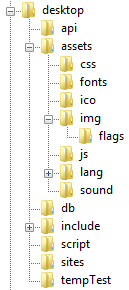
\includegraphics[width=0.25\textwidth]{images/folderStructure.png}
        \caption{The Code Folder Structure}
        \label{fig:folderStructure}
\end{figure}

\noindent{\textbf{desktop:} This is the main directory for the desktop version. The reason for not having a single root directory is that there might be some variations between the desktop and the Android version of the system.}\\
\\
\textbf{api:} Is intended to contain API which are not JavaScript or PHP code. And is empty as of the end of this project.\\
\\
\textbf{assets:} Contains every asset in the system. Images, JavaScript, sound, fonts, CSS and language files.\\
\\
\textbf{assets - css:} Contains the CSS files for the system.\\
\\
\textbf{assets - fonts:} Contains special fonts for the system.\\
\\
\textbf{assets - ico:} Contains the icon files for the system.\\
\\
\textbf{assets - img:} Contains the static image files for the system. Pictograms and Profile Images are loaded from the database.\\
\\
\textbf{assets - img - flags:} Contains images of flags, used for changing language.\\
\\
\textbf{assets - js:} Contains all JavaScript in the system, files are named as they fit to PHP files, as far as this is possible.\\
\\
\textbf{assets - lang:} Contains all language files to the system. Each webpage and some JavaScripts, have their own language sub-folder . Right now they contain English and Danish language files.\\
\\
\textbf{assets - sound:} Contains all static sound files to the system. Sounds for Pictograms are loaded from the database.\\
\\
\textbf{db:} Contains the database files. All active database functions are stored in the file ``new.db.php''\\
\\
\textbf{include:} Contains any JavaScript or PHP code that is not developed by the Admin project, that is included in the system.\\
\\
\textbf{script:} Contains PHP scripts which do not display anything, but rather work to execute some functions such as changing a profile image.\\
\\
\textbf{sites:} Contains .html and .php files which correspond to a webpage on the website.\\
\\
\textbf{tempTest:} A folder for any need of generating files during development.

\subsection{PHP and JavaScript}
%Why PHP and JavaScript
As already mentioned in this chapter we chose to use PHP as the back-end language. And in order to make some more advanced user interface we decided to use JavaScript, HTML and CSS as front-end languages.\\
We chose to use PHP because most of the Admin group already had experience with the language, and also because we found PAW which would make it possible to execute the PHP code on the tablet.\\
Also another bonus, which was not considered much when we made the choice, is that PHP is natively able to work with JSON objects which is how we communicate with the database API.\\
\\
JavaScript, HTML and CSS were chosen as front-end because of the product being a website, for which there is no real alternative.

\subsection{Language Support}
%Language Support
It was in the beginning of the project suggested that the system could be operated in multiple languages, as a start in Danish and English. This was suggested by the semester coordinator. The admin group thought, if this was to be implemented at any point, it should be in the beginning of the system, which meant we would have to implement it into our system.\\
The way it is implemented is much like how it is in Android applications, and can be read in further details in \vref{sec:languageSupport}.\\
\\
The reader should now have an understanding of the most basic decisions of the Admin project, and be able to navigate in our system.\\
The next chapter will go through the project progress, followed by the project's problem statement.

	\chapter{<<Project Progress}
\label{sec:projectProgress}
%Why do we explain this?
This chapter concerns the work progress of the project and the documentation here of. 
The work progress was split into weekly progress that was documented with a weekly abstract that is to be read in conjunction with sprint story.  
At the end of this chapter the reader should have the knowledge of the development structure that is used and have the overview of the work that was done in this project. 


\section{Weekly Abstracts}      
\label{subsec:weeklyAbstracts}
%Why did we make Weekly Abstracts?
Weekly abstracts are a small resume on what have been developed over a week and what problems occurred during that time. 
Usually the weekly abstract is between 5-10 lines of text that is written at the end of each week. 
Writing weekly abstracts is an easy way to ensure that the development move forward because if there is nothing to write, nothing was made and one should reflect upon that.
Also newcomers or an involved third person will be able to quickly get up to date on project status by reading the abstracts.         

\section{Weekly Progress}
\label{subsec:weeklyProgress}
%Why did we do what we did?
In the rest of the section is a description of the weekly progress in conjunction with sprint story.
The conclusion of the work progress will be at the end of this chapter. 

The first two weeks of project was used to create the groups and determine which projects should be worked on this year.  
Internal in the group the expectations was aligned and work conditions was established.
Graphic figures, including logo, and design guidelines was also established.      

Sprint stories was first used in week 3 (04/03/2013-08/03/2013).   

\textbf{Week 1 (18/02/2013-22/02/2013)} 
Designs and features for the Admin interface was discussed.
Low-fi board designs was made to give abstract view of our ideas regarding the meeting with our contact person.   
The first considerations to incorporation of multi language support.
The structure of PHP, project and report has been made so it is ready for the first sprint.
Setup GIT and Redmine.
It was agreed upon to make a web based administration system that is convertible to both desktop and tablet.  
For further information this choice is readable in chapter \vref{chap:systemDesign}.

\textbf{Week 2 (25/02/2013-01/03/2013)}
The focus has been on finishing the preliminary interface design and web application structure.
All of the interface design that was drawn on whiteboards was converted to Balsamiq mock-ups for a coherent feel.
At the meeting with the contact person there was feedback on the design and features. 
Work in committees started. 
The feedback, questions and answers regarding how the day care works can be found in appendix \vref{interviewMette}.
The Balsamiq mock-ups and web application structure is found in appendix \vref{apx:mockups} 

\textbf{Week 3 (04/03/2013-08/03/2013)}
This week work has been on implementing the design and functionality of the login screen and main navigation.  
We have also edited our mockup designs with the feedback we got from our contact person. 
Bootstrap is included to streamline the design. 

The first scrum sprint started with the main story being  our, which will last from 04/03/2013-18/03/2013. 

"The guardian is in the launcher and starts all the applications one after one, the guardian can freely move from application to launcher at any given time.
The guardian also enters the administration."

From that story we concluded the demand for our sprint was for a user to log in to the system and view his/her profile page. 

\textbf{Week 4 (11/03/2013-15/03/2013) }
The first scrum sprint is completed. 
Following sites is somehow functional implemented in the Admin system:
\begin{itemize}
        \item Log In/Out
        \item Own Profile
        \item View own information
        \item Edit own information
\end{itemize}
The site can still not be shown outside of the campus network, and therefore can it not be shown to the contact person.
Regarding functionality the site is not connected to the final database but all the dummy data is there.  
The first parts of the common report is created.

\textbf{Week 5 (18/03/2013-22/03/2013)}
Most progress was in implementing the design and edit the mock ups. The committee for the DB-API is started. This committee is important as it will define connection to the database. 

The new sprint is:
``The guardian is in a application and is working with a picture''

The focus is therefore on implementing profile pictures. 

\textbf{Week 6 (25/03/2013-29/03/2013)}
Time was short because of Easter. 
Following features was integrated the Profile Picture Edit and ability to Change QR.
Mock ups of Profiles, Create Profile and Department Management was also worked on.    

\textbf{Week 7 (02/04/2013-05/04/2013)}
This week there only were 4-8 hours of free work time, because of the many lectures and the holiday of this week.

The new sprint is as follows: 
``The guardian creates a pictogram, and imports the pictogram to an application. The guardian personalizes the application.''

\textbf{Week 8 (08/04/2013-12/04/2013)}
This week an auto update script that fetches the git-repository for our web-server were made.
Uploading the profile picture was reworked to a faster and more data efficient way. 
But still missing the database to store the data and to give a report when the image fails to upload or succeeds.
The QR generators is now fully functional. 
There is now a printer function to send our QR-images to the browser or OS printing service.
\\
\textbf{Week 9 (15/04/2013-19/04/2013)}
The QR system is changed, so that it is secure. 
Language support now work for all the developed sites. \\

\textbf{Week 10 (22/04/2013-26/04/2013)}
Uploading of profile picture is finished.
The work is now on getting the Admin interface down to the tablet.
We have scheduled a meeting with Mette Als (our contact person), to test our system. 

New sprint: 
``The guardian can navigate between applications and use them''
\\
\textbf{Week 11 (29/04/2013-03/05/2013)}
This week were used on solving the whole problem with the missing database.
A front end was created for the Picto Admin. Features  in our system can not be supported in IE9 and below. therefore is a warning has been added at the log-in page that informs the user that they are using an old browser if the browser does not support the ``FileReader'' system in JavaScript.

\textbf{Week 12 (06/05/2013-10/05/2013)}
The week was used to prepare for the usability tests(Monday the 13th).
Profile Create and Make Relations got finished, with exception of the DB create implementation. 
Also Picto Admin Create is fully finished. But it does not support categories. 
In the weekend between the 10th and the 13th was used to ensure that the system could work with the newly developed database API. The system was not ready in time for the usability tests. 

\textbf{Week 13 (13/05/2013-17/05/2013)}
The tests was completed and analyzed. 
All the bugs and wanted changes got documented and set to be fixed.
Most of the week was used on implementing the DB API in the system and make fixes.     
The report structure was made and writing of the report has been started. 
The finished functionality can be found in chapter \vref{chap:systemOverview}.
 
At the end of the project the program was tuned to be fully functional and include notes.
Until the report delivery was writing documentation.       

\section{Conclusion of Project Progress}
The weekly abstracts was a good point to acknowledge the progress and evaluate the work effort. It was also used to inform our supervisor of the progress we made during the project
The group work process was more a natural development process forced by the sprint story.       
The one thing that did complicated the work was the lack of cooperation with WASTELAND that should have been much closer. 
\label{sec:conclusionofProjectProgress}


	\chapter{Problem Statement}
\label{chap:problemStatment}
The general purpose for this project has been explained both in this reports introduction and in the GIRAF introduction, see the Introduction\vref{introduction} and \ref{sec:admin}.

The first GIRAF Admin project was started in 2011, then in 2012 it was split into two projects, called Savannah and Oasis. The two last named projects were focused on constructing database systems as well as user interfaces to support it. Savannah was implemented as a web version and Oasis as a tablet version. When the two projects were finished, the databases could not synchronise and was at this project's start ultimately scrapped due to incompatibility and low maintainability.\\
In 2013 the projects were split into constructing an administration interface and constructing a proper synchronisable database. The database project this year was named Wasteland \citep{wasteland}.\\

Since Wasteland chose to redesign the database in order to accommodate the use on several platforms and synchronisation, it was a logical choice to also redesign the administration interface, seeing that a database design would render previous projects work useless. This also accommodated a way to heighten maintainability and user friendliness. This will hopefully ensure that this administration system will not be discarded next year.\\
In order to fulfil the general need of user creation in the GIRAF system, the focus will have to be on creating all the profile management tools first. This means that if some of the features cannot be implemented in time, as explained in \vref{chap:systemOverview}, then the focus should be on the user management interface. This will leave all management of pictograms to the tablet projects.

This has lead to the following problem statement:
\begin{verse}
\textit{``Currently there are two different administration interfaces for the GIRAF system.
This results in a problem with maintainability and user friendliness.
How can we make a \underline{single} user friendly administration interface for the GIRAF system?''}
\end{verse}

	\newpage
%\addtocounter{page}{1}
\thispagestyle{empty}
\mbox{}
	
	
	% Part Solution
	\part{Solution}
	
	\chapter{System Overview}
\label{chap:systemOverview}
%What will this chapter contain
In this chapter we give an overview of the features that the system contains, their status and why they are necessary.

Below is shown a table containing each feature that we have designed. As can be seen by table \ref{tab:FeatureTable} we have designed a few features that we think is necessary for the online PC system. It can also be seen that we only managed to finish 3 out of 12 features and 4 out of 12 is only in need of DB implementation. That leaves 5 out of 12 features unstarted, where 4 of these are related to the Pics Manager.

%Tabel of System functions, with completion status
\begin{table}[htbp]
	\centering
		\begin{tabular}{|l|l|}
			\hline
			Feature Name & Status\\\hline
			My Profile & Done\\\hline
			Profiles & Done\\\hline
			Create Profile & Needing DB\\\hline
			Add Relation & Needing DB\\\hline
			Pics Manager - Make & Done\\\hline
			Pics Manager - Add & Unstarted\\\hline
			Pics Manager - Remove & Unstarted\\\hline
			Pics Manager - Edit & Unstarted\\\hline
			Pics Manager - Delete & Unstarted\\\hline
			Dep. Information & Needing DB\\\hline
			QR Manager & Needing DB\\\hline
			App Manager & Unstarted\\\hline
		\end{tabular}
	\caption{Feature Table - The status explain if they have been finished or not}
	\label{tab:FeatureTable}
\end{table}

As it can also be seen from the table we have focused on implementing features that makes it possible to handle Profile related issues. This have been done because it is already possible to handle pictograms from the tablet systems.\\
We did implement one of the Pics Manager features, Make, this is due to it not being system wise directly connect to the remaining 4. The 4 remaining features of the Pics Manager are all based on the same search and select system and should therefore not prove difficult to implement at a later point. But more on this later, see chapter \vref{chap:futureWork}.


%Short explanation of each functions feature
\section{My Profile}
Status: Done\\
Resume: This feature displays the logged in users information as well as the users relations and makes it possible to change these information. My Profile also has a sub feature to change the Profile Image of a user, which will be explained in further detail in section \vref{sec:profilePicChange}.

\section{Profiles}
Status: Done\\
Resume: This feature is an admin feature, it displays all profiles in a department that have been related to a pedagog in some way. It also makes it possible to navigate to these profiles.

\section{Create Profile}
Status: Needing DB\\
Resume: This feature is an admin feature, it makes it possible to create new profiles for a department. But is not able to give admin rights to a user. Admin rights can only be given directly from the Database.

\section{Add Relation}
Status: Needing DB\\
Resume: This feature is an admin feature, it makes it possible to form relations between children and pedagogs, as well as children and parents.

\section{Pics Manager - Make}
Status: Done\\
Resume: This feature makes it possible to create pictograms.

\section{Pics Manager - Add}
Status: Unstarted\\
Resume: This feature makes it possible to link a pictogram to one or more children.

\section{Pics Manager - Remove}
Status: Unstarted\\
Resume: This feature makes it possible to remove a link to a pictogram from one or more children.

\section{Pics Manager - Edit}
Status: Unstarted\\
Resume: This feature makes it possible to edit a pictogram that have been already created in the database.

\section{Pics Manager - Delete}
Status: Unstarted\\
Resume: This feature makes it possible to permanently remove a pictogram from the system.

\section{Dep. Information}
Status: Needing DB\\
Resume: This feature is an admin feature and makes it possible to edit the information about a department.

\section{QR Manager}
Status: Needing DB\\
Resume: This feature is an admin feature and makes it possible to change the QR key for a user.

\section{App Manager}
Status: Unstarted\\
Resume: This feature is for adding or removing the rights to use an application for a child, and is the only feature still in the design step.

This chapter should now have given a proper overview of the systems features, and it should be clear what the system is intended for and how. The next chapter will explain how we designed the system, followed by a deeper explanation of some of the more advanced features in the system.
	\chapter{Design}
\label{chp:design}
This chapter will describe the design procces of the administraion system.\\
Seeing as the work from previous years will not continue in this project the opportunity to make a new design filosophy rose. 
In 2012 the Luancher group made a design guide. This guide was extended in the Design committee\fxnote{ref til design guide} and this project will follow that guide. Basecally it says that one should follow the color theme \fxnote{insert relation to appendix with color-theme} and use vector graphics as much as possible. \\
Looking at other web administration interfaces like Wordpress\fxnote{insert wordpress ref here} the general idea of having a navigation bar at the left side of the screen and the conteent for a given menu on the right side as \ref{fig:ideaWep} shows. This idea also came from the Android systems settings app, which looks like wordpress admin interface but include a more nuetral way of displaying catagories. The login page, which is the only page that does not follow the genral idea, is inspired directly from Twiiter's \fxnote{twitter ref} Bootstrap sign in layout.\\ 
Every menu-item went through the same procces of using a whiteboard as a screen and then draw the design in hand. Afterwards the hand-drawm mockups was  created as digital mockups in Balsamiq Mockups \fxnote{ref}. Then at a meeting showed to our contact person and changed to reflect the issues risen by her. The complete set of final mockups are available in \ref{apx:mockups}.\\

\begin{figure}[!h]
\centering
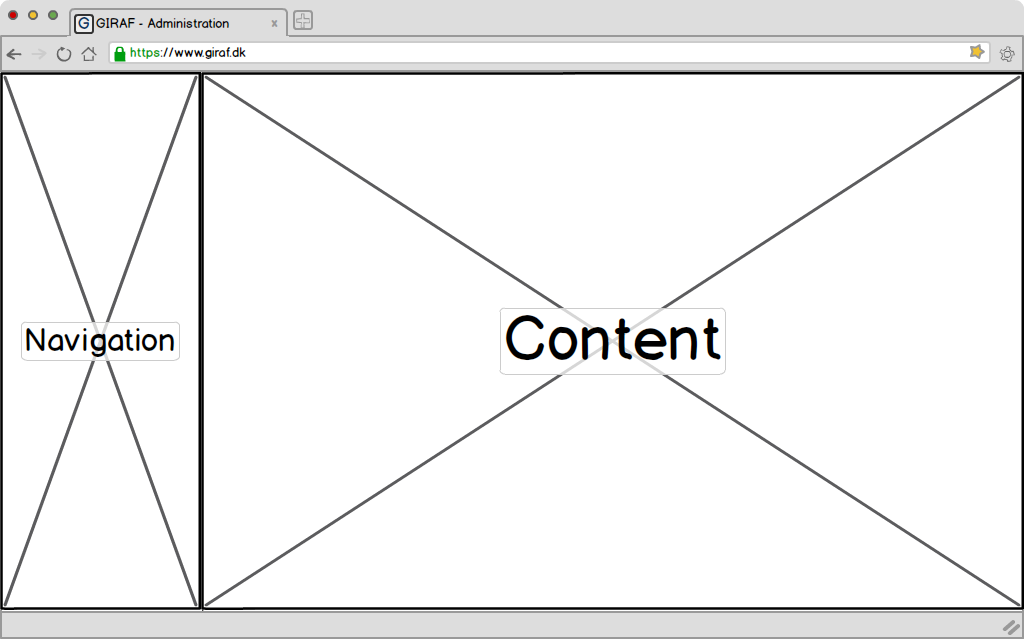
\includegraphics[width=1\textwidth]{images/mockup/displayMode.png}
\caption{General idea of building web-pages.}
\label{fig:ideaWep}
\end{figure}


\section{Designing individual pages}
\subsection{Login}
The Login page is designed to be as minimal as possible. There should be no cluttered information and with a single exeption no other option than to login, the exeption being changing language. The mockup is viewable on figure \ref{fig:loginDesign}.
\begin{figure}[p]
\centering
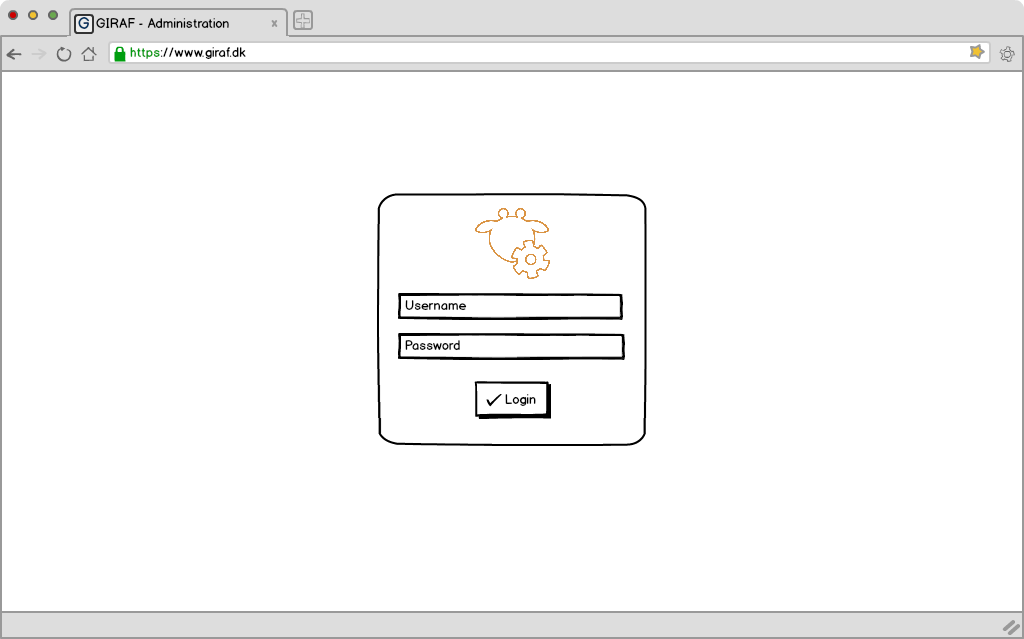
\includegraphics[width=1\textwidth]{images/mockup/login.png}
\caption{Login}
\label{fig:loginDesign}
\end{figure}

\subsection{Navigation}
Navigation was one the design items that went through a lot of small changes. The general idea being that it should look an feel natural to an android user. This being that the navigation bar conforms to a principle about accessability so that there is no foldout points or other elements that would be considered diffucult to get to on a touch screen. On the mockups each menu category has a little image next to it, this is changed so that now the first letter is capatalised and uses a bigger font than the rest of the test. If a user with administrator rights login he will be able to see all menu items but if a user with degrated rights logs in he will only see Own Profile, Pics Manager and App Manager further information about  department for an example is then accesible through own profile without editting rihgts.  A mockup showing the navigation and the profile page is figure \ref{fig:own_profileDesign}.
\begin{figure}[p]
\centering
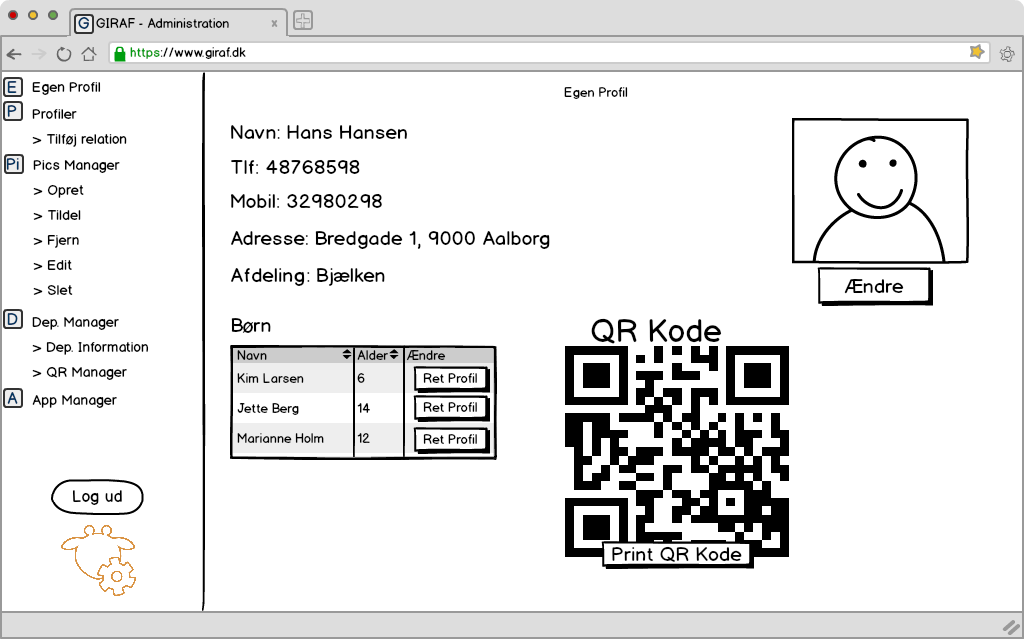
\includegraphics[width=1\textwidth]{images/mockup/egenProfil.png}
\caption{Navigation and Profile page}
\label{fig:own_profileDesign}
\end{figure}

\subsection{Profile Page}
The profile page is the page that is showed when a user logs in. It should have information about the user as well as information about linked profiles such as attached children, parents or pedagouges. A user should also be able to edit his own information as well as attached childrens information. As a result of our usability test \ref{chap:usabilityTesting} the current design used does not include the abillity to change ones QR-code. Instead only the Ddepartment manager has that abillity. A mockup showing the navigation and the profile page before usability testing is figure \ref{fig:own_profileDesign}.

\subsection{Profiles}
It is based on the idea that having a complete overview of how things are linked sometimes gives a better overview and therefore it is designed such that all links between pedagouges, children and their parents are displayed in an easy to comprehend way. To do this we agreed upon a single table approach which gracefully full-fills the comprehension wanted. This is even more underpinned when color coding is applied to guide the user.
\subsubsection*{Create Profile}
The title basecally says everything. Here the point is that one, if privileged, would be able to create other profiles. A number of input fields as weel as the option to select which type of user one want to create is what this page consits of.
\subsubsection*{Add relation}
Here a privileged user should be able to create relations or links between other profiles. A scenario would be that a child profile has just been created and it should now be linked to it's alreade created parents. This procedure should take place here.

\subsection{Pics Manager}
Pics Manager is based opun having the capabillity to create, add, remove, edit and delete pictograms which all are designed to the same principles of easy accessibility as the rest of the system. Pics Manager should not be accessible on tablets. This is mostly due to the fact that sepperate applications has been developed for it's primary purpose. It should instead open theese apllications and the user should not be bothered by this. The different components design should have the same look and feel as the android application but take advantage of the fact that they are run on a dektop computer and not a tablet.
\subsubsection*{Create}
Originalle named Make this tool should supply the user with the capability to create pictograms in the database.
\subsubsection*{Add}
Add pictograms to users.
\subsubsection*{Remove}
Remove pictograms from users.
\subsubsection*{Edit}
Enables the user to edit pictograms that the user has available.
\subsubsection*{Delete}
If a user own a pictogram he can delete it permanently from the database.

\subsection{Department Manager}
Enables a privileged user to edit department infomartion and view a shortlist of attached pedagouges.
\subsubsection*{Department Information}
Essentially the same as Department Manager but displays the information as an unprivileged user would see it. An unprivileged user accesees the page through a link on his profile page.
\subsubsection*{QR mamanger}
Enables a privileged user to change users qr-codes. This is also one of the pages that have gone through a number of deisgn itterations. as viewable in \ref{apx:mockups} it originally had three sub items but was refinded to a single page with a much more comprehensive layout. This enables the user to complete a given task much more easaly. A screenshot of the current lauoyt is \ref{fig:fig:qrManagerCurrentDesign}
\begin{figure}[p]
\centering
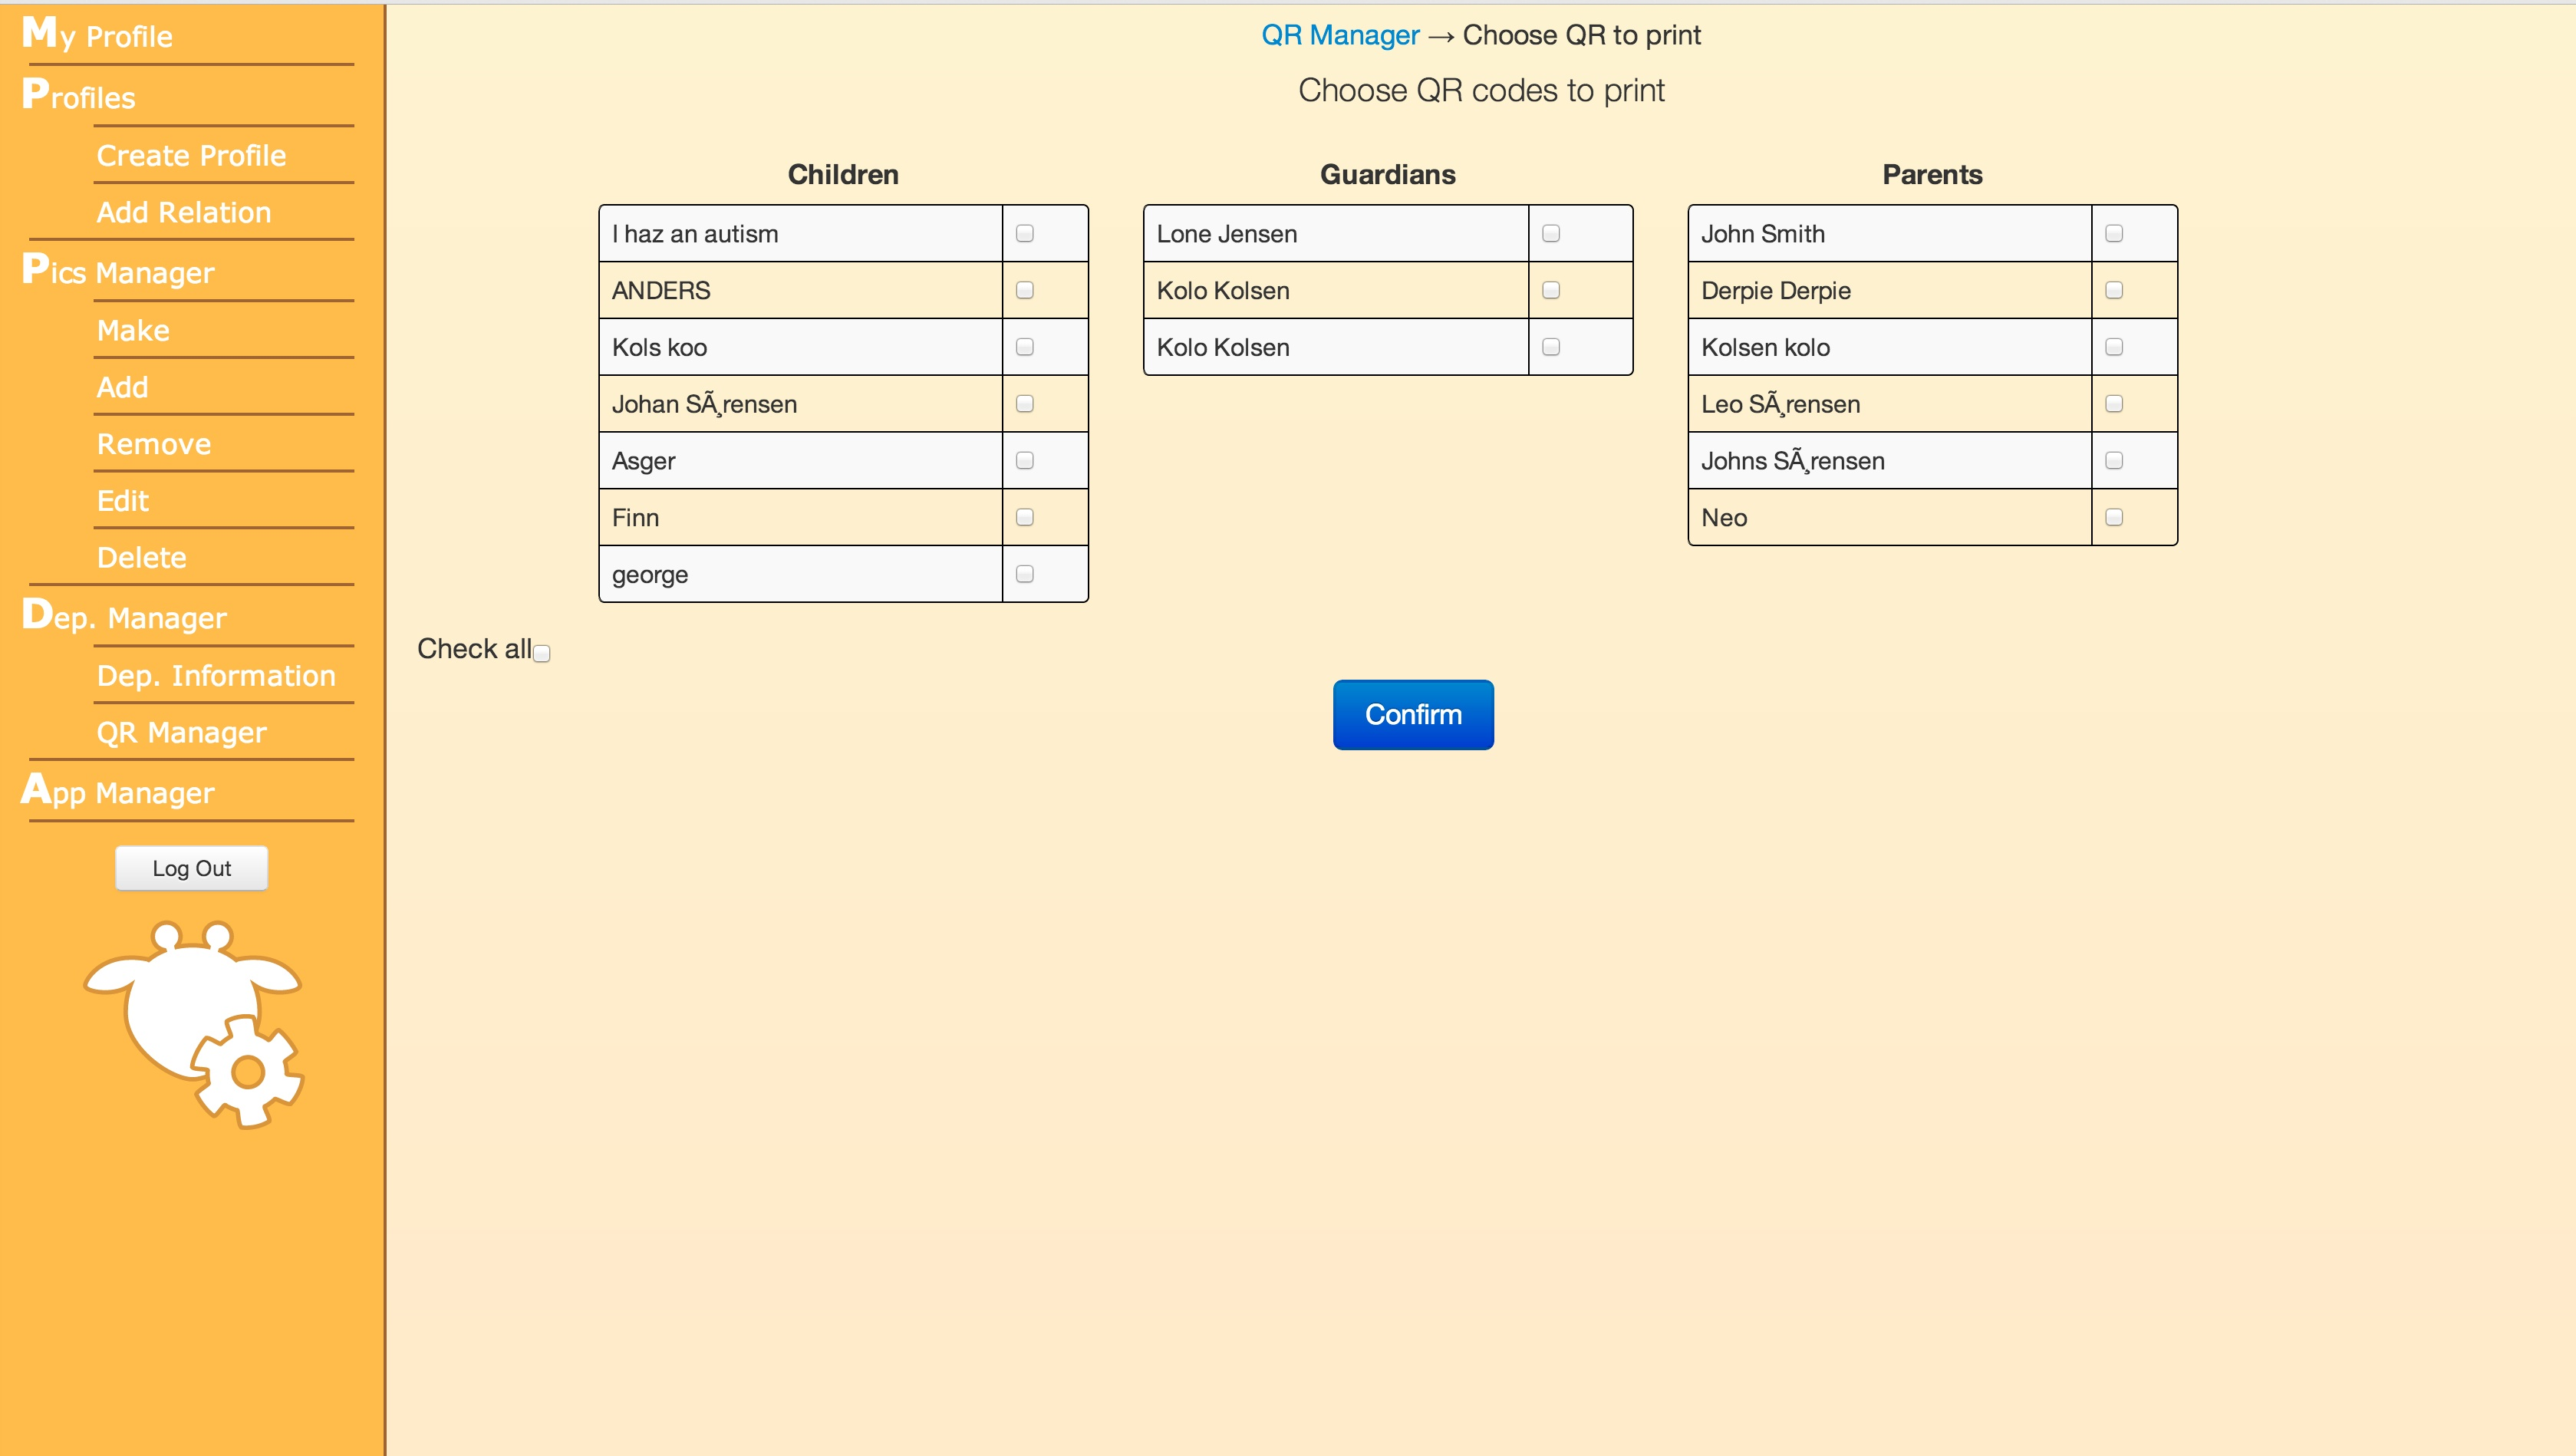
\includegraphics[width=1\textwidth]{images/mockup/qrManagerCurrent.jpg}
\caption{Current design of QR manager}
\label{fig:qrManagerCurrentDesign}
\end{figure} %Design står her i vores opsætning
	\chapter{Implementation}
This chapter is about implementation...
	\section{Navigation}
\label{sec:navigation}
%Why do we explain this?
The navigation system that we have implemented in our system is based on JavaScript and the event \texttt{window.onhashchange}, with the addition of Ajax.
We use Ajax to fetch the sites without ever navigating away from the index site. This is done because we wanted to minimize the amount of data transfer from the server that the site is made on. However this do present itself with a few challenges. For example we have had to come up with a special solution in order to send the PHP \texttt{\$\_POST} and \texttt{\$\_GET} data around, in this section we will explain how this is implemented and how it should be used in the future.\\
\\
%Why did we make it so complex?
	%Alternative solutions
But first we will elaborate on the alternatives that was available to us.\\
There is at least two other solutions that could have been implemented with different advantages. First we could have implemented the old HTML method, which means that the user would have to navigate directly to the files name. This would be an easy way to build the website, but would leave it very hard to maintain, since the design of the website would have to be written more than one place, or at least use an include in the top and bottom of each page.\\
Another alternative would have been the use of a PHP based switch. The method is commonly used in larger website systems, because it makes for easy design and maintainability.
\lstset{language=PHP}
\begin{figure}[htbp]
\begin{lstlisting}[firstline=1]
	$site = $_GET['site'];
	switch ($site) {
    case "ownProfile":
        include "sites/ownProfile.php";
        break;
    case "picsMake":
        include "sites/picsMake.php";
        break;
    case "":
		default:
        include "sites/home.php";
        break;
	}
\end{lstlisting}
\caption{A PHP switch Example}
\label{lst:phpSwitch}
\end{figure}

As seen in listing \ref{lst:phpSwitch} it is easy to create the switch method, and maintain it, since all that is needed is to add another case when a new site is made.\\
What listing \ref{lst:phpSwitch} contains has to be included in the index.php file, and the links, or hyperlinks, will have to set the \texttt{\$\_GET} variable \texttt{site} to a fitting name for the site, and it will then include the content of that site.\\
\\
However this PHP switch solution has one downside to it. It still sends the data of the index file from the server to the user each time the user presses a link. This might not be much data, but it becomes so in the long run. We therefore went with a third alternative, which is much like the PHP switch method. We simply took the same idea and wrote it in JavaScript, this however means that we must use Ajax to perform the fetching of new data.\\
\lstset{language=Java}
\begin{figure}[htbp]
\begin{lstlisting}[firstline=1]
switch(destination)
	{
		case "":
		case "#ownProfile":
		case "#otherProfiles":
			destinationPath = "sites/own_profile.php";
		break;
		
		case "#profiles":
			destinationPath = "sites/profiles.php";
		break;
		
		case "#profilePicUpload":
			destinationPath = "script/profilePicUpload.php";
		break;
		
		...
		
	}
	
	...
	
	$.ajax({
		type: "POST",
		url: destinationPath,
		data: postData,
		success: function(result) { // result is the content that the php file 'ECHO's.
			$("#content").html(result);
		}
	});
\end{lstlisting}
\caption{The JavaScript switch}
\label{lst:javascriptSwitch}
\end{figure}

%POST Transfer
Listing \ref{lst:javascriptSwitch} contains the main contents of the JavaScript switch that we created. \texttt{destination} is the variable that we use for storing the actual hash value\footnote{Hash value is the value followed by the hash symbol \# in hyperlinks.} and the \texttt{postData} is created in a unique way, so that we can send the PHP \texttt{\$\_POST} data on to the site that the JavaScript is Ajax'ing to.\\
%File list
\lstset{language=PHP}
\begin{figure}[htbp]
\begin{lstlisting}[firstline=1]
	echo "<script>
		var postData = ";
		echo json_encode($_POST);
	echo "</script>";
\end{lstlisting}
\caption{The POST transform code}
\label{lst:postTransform}
\end{figure}

As seen in listing \ref{lst:postTransform} we convert the \texttt{\$\_POST} data from PHP into a JavaScript variable that then again is send on to the next PHP site as seen in listing \ref{lst:javascriptSwitch}.\\
\\
%Syntax
However we also wanted to be able to use the \texttt{\$\_GET} variable from PHP on other sites that we call with Ajax. In order to do this we created a rule as can be seen in listing \ref{lst:getData}, the rule says that instead of using the usual syntax of ''?'' after the hyperlink, there needs to be a ''/'' instead. We do this because we think it gives a better look on the link itself.\\

\lstset{language=Java}
\begin{figure}[htbp]
\begin{lstlisting}[firstline=1]
    var hashInfo = location.hash;    
	var hashArray = hashInfo.split("/"); // We use / instead of ? in our URL's (for $_GET), they do the exact same, but gives a different look
	var destination = hashArray[0];
	var info = hashArray[1];
	var destinationPath = "";
\end{lstlisting}
\caption{The GET transform code}
\label{lst:getData}
\end{figure}

Then when the code in listing \ref{lst:getData} and the switch in \ref{lst:javascriptSwitch} has been executed we append \texttt{info} to \texttt{destinationPath} with the normal syntax. Then the Ajax call does the rest.\\
\\
But this method also has a bad side. It requires a more complex way of calling scripts that is dependent on large amounts of data from the user. For example when the user wish to upload an image for a pictogram.\\
As seen in listing \ref{lst:largePost} which is a cutout of the \texttt{headInclude.php} file, which is always included in our \texttt{index.php} file, we include the script directly into the index file instead of using our special Ajax JavaScript function. If we did not do this, the user would have to send the data to the server twice. First in order to send it to the index file, then the user will receive it again, and then call the Ajax function with the same data.\\

\lstset{language=PHP}
\begin{figure}[htbp]
\begin{lstlisting}[firstline=1]
	if(isset($_POST['picsManagerMakeSubmit'])){
		//Call upload script
		require "script/picsManagerMakeUpload.php";
	}
\end{lstlisting}
\caption{The handling of big PHP POSTs}
\label{lst:largePost}
\end{figure}

And then the upload script must always make sure to use a PHP \texttt{header} call to navigate the user to the right site, depending on whether he got an error or not.\\
\\
If the reader wants to learn more about the navigation script the files used for this script is: \texttt{/include/headInclude.php} , \texttt{/assets/js/navigation.js} and \texttt{index.php} .


	\section{QR Code Generation and Printing}
The multi-group last year decided that QR codes would be used as the only login method on tablets, which meant that the GIRAF administration system would need a system for generating and printing new QR codes, in the event a person lost their QR code. In collaboration with WASTELAND it was decided that it would be a security risk to allow people to print out existing QR codes, which meant that our system only has to facilitate the generation of new QR codes and the printing of those new QR codes. The last multi-group also decided that the QR codes would be based on a 512 character long string. The system generates the new QR codes using the code displayed in \autoref{lst:qrcode}. The QR code generation uses the function microtime in order to get data to hash. The function microtime relies on the system call gettimeofday, which means that this implementation will only work on UNIX based systems and Windows (PHP supplies its own implementation on Windows). The time from microtime is then hashed with the sha512 hashing function which generates a 128 hexadecimal long string. This is then repeated 3 more times in order to get a 512 hexadecimal long string, which is then the newly generated QR code.
\begin{figure}[htbp]
\begin{lstlisting}
function generateNewQr()
{
	$qr = "";
	for ($i=0; $i < 4; $i++) { 
		$time = microtime();
		$qr .= hash("sha512",$time);
		usleep(100); // sleep for 100 microseconds (0.1 milliseconds) to get a different time from microtime
	}
	return $qr;
}
\end{lstlisting}
\caption{QR Code Generation}
\label{lst:qrcode}
\end{figure}
The newly generated QR code is then inserted into the GIRAF database using the WASTELAND database API. Now the user is prompted to print out the new QR code, as this is the only chance the user has, without generating yet another new QR code. The PHP library phpqrcode\citep{phpqrcode} is used to generate the QR code itself into an image. In order to support the scalability of the QR code, the image is generated as an SVG, but because the original implementation of phpqrcode does not support SVG output, a modification of phpqrcode is used\citep{phpqrcodet0k4rt} which adds support for SVG and EPS. Due to a bug with Internet Explorer, phpqrcode was further modified so that the colour of the QR code is statically black. The bug with Internet Explorer was that phpqrcode would truncate the hex code of the colour black to #0 which in Internet Explorer would display as white, while in other browsers it would display as black. \\
After phpqrcode has generated the SVG, it is then added to a hidden iframe, which only contains the SVG and a separate CSS file which contains the style for printing the QR code. Javascript is then used to open the printing dialogue of the browser with the iframe as its focus, so that only the QR code is printed and not the whole page.

	\section{Profile Picture Change}
\label{sec:profilePicChange}
%Why do we explain this?
The changing of a profile picture is normally a very easy task and can be done with a simple uploading of a file and transforming it into the right size with the build in PHP functions.\\
But in our system it is a bit more complex. Both because we store the images in the Database, so that they can be retrieved on the tablet as well as our PC version. And also because of the before mentioned way we move data around, see section \ref{sec:navigation}.\\
\\
%Why did we make it so complex?
	%Alternative solutions
As again, mentioned in one of the former sections, see section \ref{sec:navigation}, we have made our system this complex in order to minimize the data transferal from the server. This forces us to make some complex solutions to anything that requires big data transferals.\\
As for the database, it is generally bad practice to store images in a database, because of the encoding that is needed to do so. But exactly because we want to be able to use the image both on the tablet and on the website, this is actually a good solution. There might have been some alternatives to this, but this is not part of our project. For more information on this the reader should read the WASTELAND project report, that also is a project under the GIRAF project.\\
\\	
%How does the data transfer
As explained in the end of section \ref{sec:navigation}, we have made it so that the upload script is called on submit, from the index files, see listing \ref{lst:largePost}.\\
In order to submit the user must go to the profile page, press the ''Edit'' button underneath the display of the profile picture, they will then be meet with a modal window\footnote{A modal window is a sort of pop-up window on a website.} where they are asked to chose a file.

\begin{figure}[htbp]
	\centering
		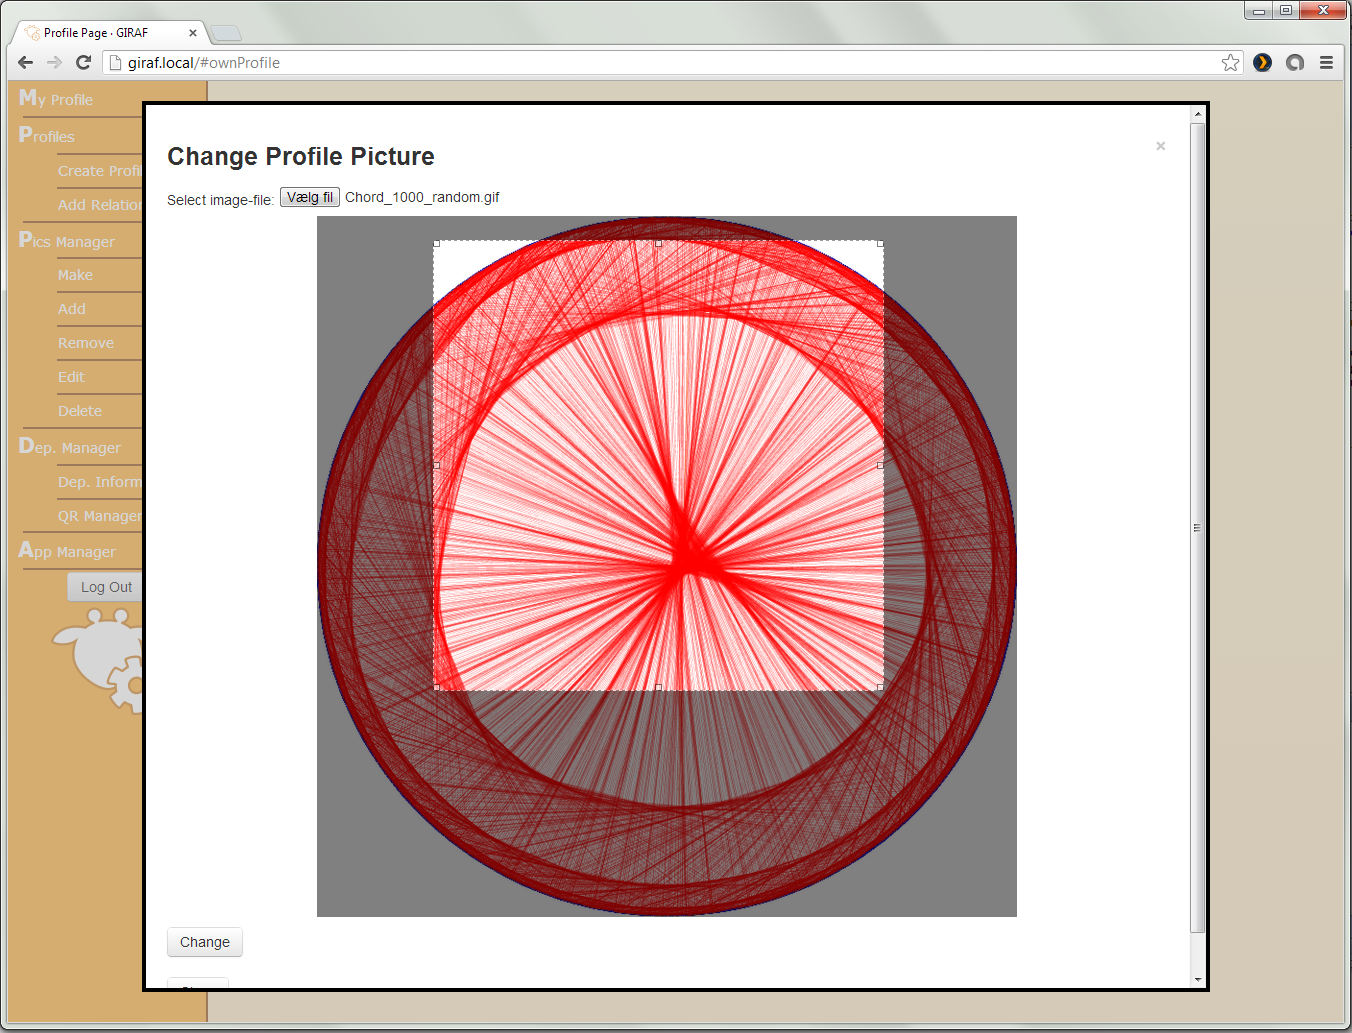
\includegraphics[width=0.50\textwidth]{images/profilePicChange.png}
	\caption{Changing a profile picture}
	\label{fig:profilePicChange}
\end{figure}

When that file is chosen they have to crop the image, as shown on figure \ref{fig:profilePicChange}, and finish by pressing the ''Change'' button.
The cropping here is made with the help of a freeware project called imgAreaSelect \citep{imgAreaSelect}.\\
Then when this is done the user will be send back to the profile site, with a success or an error message and also be able to see the new profile image on the profile.\\
\\
But what the user does not see is that on submit they are actually navigated to our profilePicUpload script, that then navigates them back with the error or success message in the URL.\\
It is this script that handles the encoding and the database query for updating the profile picture.\\
\\
When the profile picture is uploaded the script first check for any possible upload errors, as well as making sure that the file is actually an image and it was send from our form. This is to prevent security issues.
Then when that is handled, the script will load the image into PHP and will transform it by the help of a specialized cropping tool inspired by a PHP project called SimpleImage \citep{simpleimage}.\\
\\

\lstset{language=PHP}
\begin{figure}[htbp]
\begin{lstlisting}[firstline=1]
   function resizeCordsColor($width,$height,$x1,$y1,$x2,$y2,$red,$green,$blue) {
      $new_image = imagecreatetruecolor($width, $height);
			$white_image = imagecolorallocate($new_image, $red, $green, $blue); //Change image color to: White (RGB format)
			imagefill($new_image,0,0,$white_image);
      imagecopyresampled($new_image, $this->image, 0, 0, $x1, $y1, $width, $height, $x2-$x1, $y2-$y1);
	  
      $this->image = $new_image;
   }
\end{lstlisting}
\caption{The function used for cropping a profile image.}
\label{lst:croppingProfile}
\end{figure}

The function seen in listing \ref{lst:croppingProfile} is what we use for reshaping the image into a more manageable size. What it does is first create a new fully white image (L. 2-4), because it is called with the RGB value 255,255,255. Then it proceeds to copy the selected area, that the user selected before onto this white image (L. 5), in a 300 x 300 pixel area, which is the size we decided a profile picture always will be. Finally it stores itself in its own class (L. 7).\\
\\
As for implementing the database query, we have actually designed it and according to the WASTELAND API \citep{wastelandApi} it should work. But when we try to update the image it only returns an SQL error in the console. We have asked the WASTELAND group why this is, but they are as clueless as we are. So when the WASTELAND group manages to find the error, this feature will be fully implemented.\\
\\
This concludes the explanation of the Profile Picture Changer, if the reader wants to learn more about the Profile Picture Changer the files used for this feature is: \texttt{/include/SimpleImage.php} , \texttt{/assets/js/profileEdit.js} and \texttt{script/profilePicUpload.php} .








%Example of query

%Example of encoding
	\section{Multi-language Support}
\label{sec:languageSupport}
Android has simple multi-language support, which means that in order for GIRAF Admin to stay consistent with the GIRAF suite of apps, it should also support multiple languages easily. In order to make it as easy for developers to add support for more languages in GIRAF Admin a simple language system was developed. The system consists of separate PHP files for each sub-site and language. Each sub-site has a sub-folder in \texttt{assets/lang} in which all of the language files should be. Each language has a separate file with the format \texttt{sub-site.language.php}. These files then contain an associative array of strings which contains all of the static strings of the given sub-site. The language of the site is chosen when the user first logins. Each language currently has a flag below the login box on the login site, and so to change language the user just has to click on the flag of the given language. The chosen language is set in the users PHP session, and so all sub-sites has to do is check the session variable and then include the language file for that language. This can be read in detail in section \vref{sec:phpSesion}. \\

\subsection{Adding a new language}
Described here is the procedure for adding new languages into the multi-language system
\begin{enumerate}
\item For each folder(sub-site) in \texttt{assets/lang} a new file should be created with the format \texttt{sub-site.language.fileext} where fileext is either \texttt{php} or \texttt{js} depending on if the language file is for PHP or Javascript.
\item Copy all of the variables from an existing language file into the new language file and translate all of the strings into the new language
\item In \texttt{login.php} add the new flag for the new language and give it a link to \texttt{login.php?lang=language} where language is the ISO 3166-1 alpha-2 code of the given languages country (although \texttt{en} is used to designate English). When the number of flags increase to a number that can no longer be shown visually pleasing, the selection should switch an alternative selecting method more suited for large amounts of languages
\item For each sub-site's PHP file (\texttt{sub-site.php}) add the new language to the switch statement and include the language files for the new language for that given sub-site
\end{enumerate}

\subsection{Adding a new sub-site}
Described here is the procedure for adding a new sub-site to the multi-language system
\begin{enumerate}
\item On the new sub-site locate all of the static strings, and replace them with references to an associative array like this \texttt{\$SUB-SITE\_STRINGS['STATIC-STRING-NAME'] }
\item Add code to get the current language from session and a switch case statement to include the language files at the top of the PHP file in the format shown in \autoref{lst:languageswitchcase}.
\item Create a folder for the new sub-site in \texttt{assets/lang}
\item Create a new file for each of the currently supported languages in the format \texttt{sub-site.language.php}.
\item In each of the new language files create the associative array referenced earlier and add all of the strings with their translation
\end{enumerate}
\begin{figure}[htbp]
\begin{lstlisting}
session_start();
if (isset($_SESSION['lang'])) {$lang = $_SESSION['lang'];} else {$lang = 'en';}

switch ($lang) {
	case 'en':
		include($_SERVER['DOCUMENT_ROOT'].'/assets/lang/sub-site/sub-site.en.php');
		break;
	case 'dk':
		include($_SERVER['DOCUMENT_ROOT'].'/assets/lang/sub-site/sub-site.dk.php');
		break;
	default:
		include($_SERVER['DOCUMENT_ROOT'].'/assets/lang/sub-site/sub-site.en.php');
		break;
}
\end{lstlisting}
\caption{Including language support on a sub-site}
\label{lst:languageswitchcase}
\end{figure}
	\section{Pics Manager - Make}
%The similarities with Profile Pics Changer
The way the Pics Manager - Make feature is implemented is very similar to how the Profile Picture Changer is implemented, see section \ref{sec:profilePicChange}.\\
They both get called the same way and both rely on the HTML Form Element to receive their data. They also give back their error message in the same way.\\
\\
%The special user interface
But what is more interesting is their differences. Looking at figure \ref{fig:picsManagerMake} it can be seen how the user interface is designed. The top left part is for entering the general data, and the right side is for the image and the sound file.\\
\\
We have designed it so that when a user chooses a sound file, or an image file, they can hear, or see, a preview of it before uploading. We also did this so that the design could be reused for the editing feature.\\
The preview is possible because of a JavaScript function called \texttt{FileReader}. Which simply loads the file into the browser, and makes it possible to work with it without uploading the file. But this is only available in some of the newer browsers. Which means we have had to disregard the use of IE9 \citep{canIUse}. In doing so we have created a warning on our login screen that checks if the \texttt{FileReader} is available, and if not the user will be meet with a warning, telling them some features will not function for them.\\
\\
\begin{figure}[htbp]
	\centering
		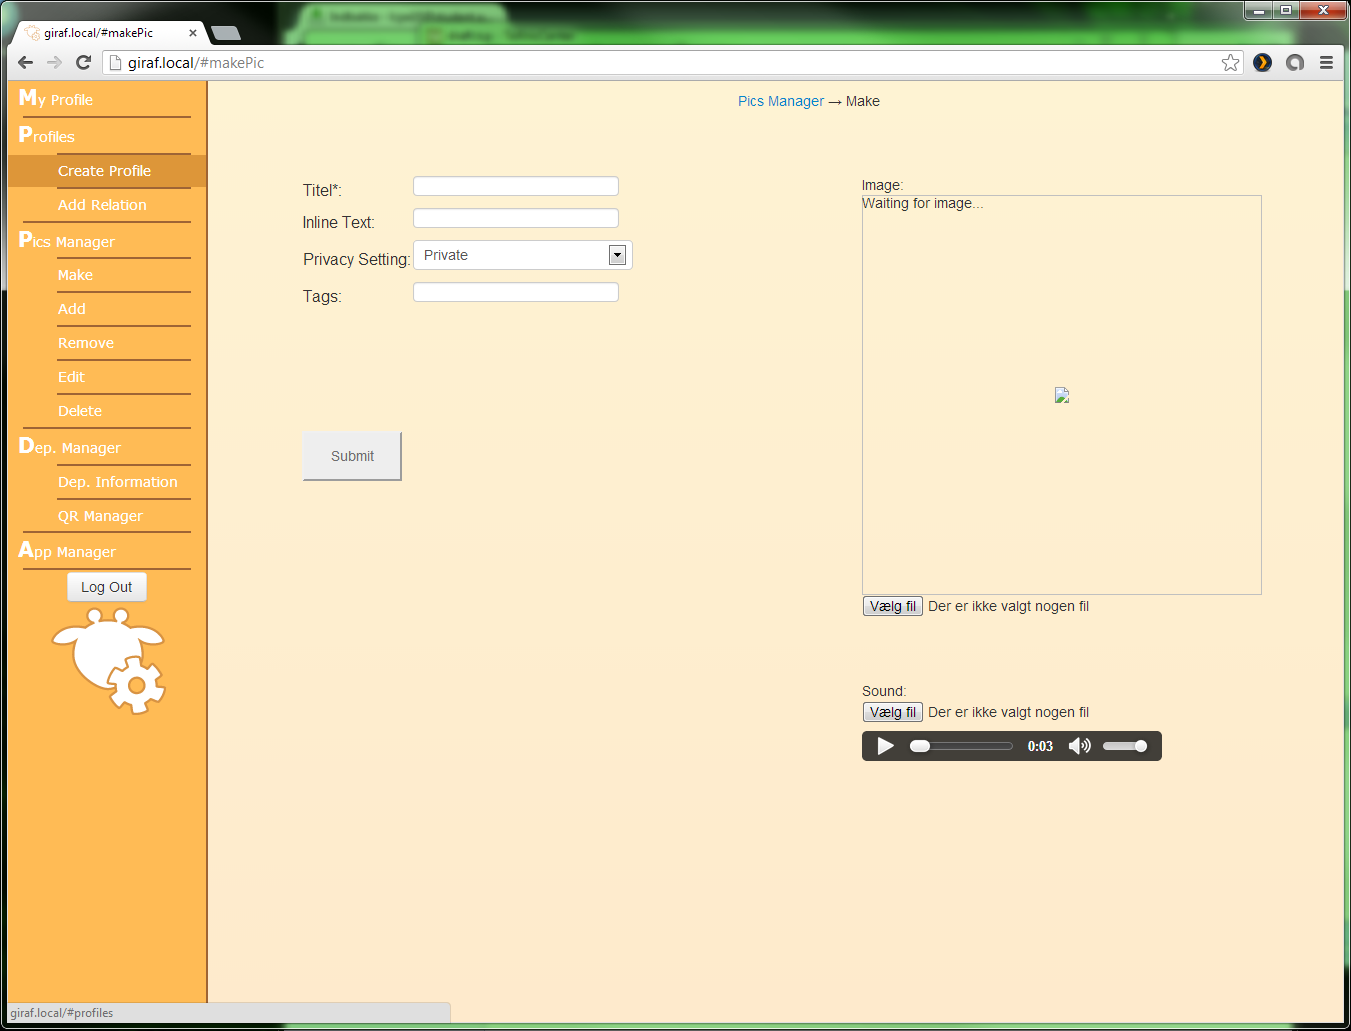
\includegraphics[width=1\textwidth]{images/picsManagerMake.png}
	\caption{The user interface for the Pics Manager - Make}
	\label{fig:picsManagerMake}
\end{figure}

%The special sound file recognizer
Again when speaking about the backend of this feature, it is very similar to the Profile Picture Changer Feature, where the main difference is that Pics Manager - Make has a specialized sound file recognizer, since this is not natively supported in PHP.\\
The function used for this can be seen in listing \ref{lst:soundFileRecognizer}, the first 2 lines (L. 2-3) creates two arrays, one for accepted mime-types and the other for accepted file extensions.\\
Next we do the actual check on file extension and mime-type. (L. 6-23), this is done by simply pulling out the information from the uploaded sound file, and see if it matches any of the variants in the arrays. This do mean that the user can upload a file with a \texttt{mp3} mime-type and a \texttt{.wav} file extension. - But since this is still an accepted sound file it is no security risk.\\
As it can be seen we use two variables which is used as booleans, \texttt{\$fileExtOkay} and \texttt{\$fileMimeTypeOkay}, these are used when we want to return the information of whether or not this was an acceptable sound file (L. 26-31).

\lstset{language=PHP}
\begin{figure}[htbp]
\begin{lstlisting}[firstline=1]
	function isAllowedSoundFile($fileName,$fileTmpName){
		$supportedExtensions = array('3gp','3gpp','flac','mp3','mid','xmf','mxmf','rtttl','rtx','ota','imy','ogg','wav');
		$supportedMimeTypes = array('audio/mpeg','audio/mp3','audio/mid','audio/wav','audio/x-wav','audio/rtx','audio/3gpp','audio/ogg','audio/mobile-xmf','audio/mxf'); //Could not find mime type of .rtttl, .ota and .imy
		
		//Check file extension
		$ext = pathinfo($fileName, PATHINFO_EXTENSION);
		if(in_array($ext,$supportedExtensions)){
			$fileExtOkay = true;
		}
		else{
			$fileExtOkay = false;
		}
		
		//Check Mime Type
		$finfo = finfo_open(FILEINFO_MIME_TYPE); // return mime type ala mimetype extension
		
		if(in_array(finfo_file($finfo, $fileTmpName),$supportedMimeTypes)){
			$fileMimeTypeOkay = true;
		}
		else{
			$fileMimeTypeOkay = false;
		}
		finfo_close($finfo);
		
		//return
		if($fileMimeTypeOkay && $fileExtOkay){
			return true;
		}
		else{
			return false;
		}
	}
\end{lstlisting}
\caption{The function used for checking sound files.}
\label{lst:soundFileRecognizer}
\end{figure}

%The DB query
	%64bit encoding

When the sound and image file have been verified they are sent on to the database query, the main part can be seen at listing \ref{lst:picsManagerMakeDbQuery}. But as also can be seen it is called with a JSON object, which we have another function for. It simply constructs a JSON string from what information the user sent us, we call this function \texttt{makeJsonPictogram}.\\
When we use the function \texttt{makeJsonPictogram} the image and the sound file is encrypted to 64 bit, which is needed in order to ensure we do not mess up the actual database query, not just the JSON object we call the WASTELAND system with. This can be done natively in PHP.\\
\\

\lstset{language=PHP}
\begin{figure}[htbp]
\begin{lstlisting}[firstline=1]
function db_uploadePictogram($jsonPictogram){
	global $session,$username,$password;
	$data = '{
		"action": "create",
		"auth": {
			"username": "'.$username.'",
			"password": "'.$password.'"
		},
	    "data": {
	    	"type":"pictogram",
	    	"values":['.$jsonPictogram.']
	    }
	}';
	
	$result = db_query($data);

	if ($result['status'] == 'OK')
	{
		return $result['data'];
	}
	else
	{
		return false;
	}
}
\end{lstlisting}
\caption{The main part of the DB query for creating Pictograms}
\label{lst:picsManagerMakeDbQuery}
\end{figure}

When the database query have been completed, the feature will as the Profile Picture Changer, send the user to the creation page with a message of success.\\
\\

%Rounding off the implementation chapter
This is the end of all the advanced and complicated solutions we have managed to complete, the next chapter will focus on the results of our usability testing of the somewhat finished system.
	\section{PHP Session Variables Overview}
\label{sec:phpSesion}
The login system of the GIRAF Admin system uses PHP sessions to check if a user is logged in. The PHP session is also populated with various variables that help the rest of the GIRAF Admin system. An overview of the different variables can be seen in \autoref{tbl:phpsession}
\begin{table}[h]
\begin{tabularx}{\linewidth}{| l | X |}
\hline
Session Variable & Description \\ \hline
\texttt{session\_id} & Stores the PHP session id of the user \\ \hline
\texttt{username} & Stores the username of the logged in user, {\color{red} Temporary variable until WASTELAND implements API session, should be removed before deploying anywhere!} \\ \hline
\texttt{password} & Stores the password of the logged in user, {\color{red} Temporary variable until WASTELAND implements API session, should be removed before deploying anywhere!} \\ \hline
\texttt{userId} & Stores the user id of the logged in user, and is used for database calls \\ \hline
\texttt{profileId} & Stores the profile id of the logged in user, and is used to reduce database calls (you can get profileId from userId) \\ \hline
\texttt{lang} & Stores the chosen language (chosen at login) of the logged in user, and is used on all sub-sites to determine what language file should be used \\ \hline
\texttt{dbsess} & Stores the database API session, which is used to make database calls after the initial login, {\color{red} this is here for future use and does not contain anything at the moment, as the database API have not implemented session yet} \\ \hline
\texttt{department} & Stores the department id that the logged in user is attached to, and is used to reduce database calls \\ \hline
\texttt{role} & Stores the role of the logged in user, and is used to determine what pages to show \\ \hline
\texttt{update} & Stores the update value of the logged in user, and is used to determine rights \\ \hline
\texttt{delete} & Stores the delete value of the logged in user, and is used to determine rights \\ \hline
\texttt{isAdmin} & Stores whether the logged in user is an admin or not, which determines what menu items should be available \\
\hline
\end{tabularx}
\caption{PHP Session Variables}
\label{tbl:phpsession}
\end{table}
Many of the variables stored in the session is used to reduce database calls, which could help the system scale better if that would be necessary. Because API session is not yet implemented by WASTELAND, it has been necessary to store the username and password of the logged in user, and is then used to make database calls instead of the session. When API session is implemented the username and password variables should be removed from PHP session and the authentication method in \texttt{new.db.php} should be replaced with API session in all calls except \texttt{db\_getSession}. At this moment it is not clear what exactly the update and delete variables signify, and the reader should refer to the WASTELAND report or source code for more details.\\
\\
%Rounding off the implementation chapter
This is the end of all the advanced and complicated solutions we have managed to complete, the next chapter will focus on the results of our usability testing of the somewhat finished system.
	\chapter{Usability Testing}
When we started this project the main reason was to simplify the administration systems to one single interface. So that there is only one code base and only one interface for the user to learn.\\
The first part should be given by default because we use a specialized system to run PHP code on the tablet. The system is called PAW \citep{paw} and is still in its beta phase.\\
The second part is the tricky part. There is only one interface to use, but it must be easy to learn and use so that the system does not have to be reworked.\\
That is why we have performed a usability test.\\
\\

%How did we do the test
	%Who was where
	%The simularity of the questions
\section{Structure of the test}
The test was performed in Cassiopeias usability lab, where we had logged the computer onto our website. The setup of the usability lab is as displayed on figure \ref{fig:usabilitylab}. We did not use the second room.\\
Each test person was lead into the test room, offered a cup of coffee and then we started the prepared briefing, everyone was given the same briefing and we asked them to sign a consent form that they were being tapped for research purposes.\\
After this we asked them to execute a set of assignments within the system, always the same assignments, designed to lead them around the whole active system. \fix{Add a refference to appendix with questions and briefing}\\
We had the same one person sit in the room to assist the user, both to give them their assignment and to tell them when they had completed it. All assignments was kept very short, as to not disturb the user more then needed.\\
When the user had completed all the assignments we had the two men that sat in the control room come and help ask questions to the test person about some of the ways the test person used the system.\\
\\

\begin{figure}[htbp]
	\centering
		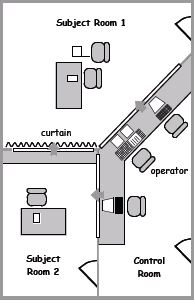
\includegraphics[width=0.40\textwidth]{images/usabilitylab.png}
	\caption{Usability Lab}
	\label{fig:usabilitylab}
\end{figure}

	%Picking the candidates
This test was only performed on 4 persons, this might not sound as many. But being that there is only a few persons in Denmark that will use the administration features that we have designed. We had to make an expert test, and use the gathered data as such. We only had one person available that we thought would use the main system that we have designed, but this person who is responsibly for a kinder garden, is not even high enough up in their system to be using most of the admin features. But this is all we had to go on, as we had no way of contacting the persons who is in a high enough position to be the intended user.\\
So the test was carried out with the one person to be the actual test person, and the 3 others be confirmation test, so that we did not draw conclusions from one test, that could be a result of lacking computer skills or other variables of the same sort.\\
3 out of the 4 test persons is working with kids with autism everyday, and is educated pedagogs, and is therefore very close to the intended user for the administration system, but is in fact the intended user for some of the sub-functionality of the system. The last test person is an educated computer scientist from Aalborg University, whom has a child with autism, this last test persons use of the system was regarded with respect to that of his education and was mainly used for catching really serious bugs and suggestions for new features.\\
\\

	%The old version
Lastly, this test was performed on, at the time, older version of the system. Because of some instabilities in the, at the time, current system. The version that was used for the test can be found on github \citep{testBranch}.\\
\\

\section{Result of the test}
Table \ref{tab:Bugs/Errors} displays the errors or bugs, that we found by the help of the usability test. They are described by first a category, if any, and then by the error itself.\\
They have been sorted by the severity of the error, and we here use 3 categories, critical, serious and cosmetic. Critical depicts an error that either makes a general task impossible or made the user stop all together. Serious depicts an error that made the user stop for some time, or seemed to be unnecessarily distracting. Cosmetic depicts an error of low caliber, that even the users informed us was minor issues that did not affect the flow much more then a few seconds.\\
\\

%Result of the test
	%Bugs/Errors
		%Severity
\begin{table}[htbp]
	\centering
		\begin{tabular}{|l|l|l|}
			\hline
			Description & Severity & Done\\\hline\hline
			It is not possible to create new categories of Pictos & Critical &\\\hline
			Profile - Restrict QR editing to department manager & Critical &  \\\hline 
			DB Problem - Not possible for all pedagogs to fix pictos for all department children & Critical & \\\hline
			Navigation - The site ''Profiles'' should link to each profile & Critical &\\\hline
			Missing - Unable to remove relations & Critical & \\\hline
			Profile Pic - Accept button is hard to find & Serious &\\\hline
			Profile Pic - Word ''change'' is misleading & Serious &\\\hline
			Navigation - ''Add'' and ''Make'' under Pics Manager is confusing & Serious & \\\hline
			Navigation - Language Support on navigation did not change to danish & Serious & Done\\\hline
			Missing - No Danish language support on the site ''Profiles''& Serious &\\\hline
			Profile - Department should be a link, not editable & Serious & (Done)\\\hline
			Profile - Links from Own Profile relations is missing & Serious & \\\hline
			Profile Pic - GIRAF Logo as Placeholder is misleading  & Cosmetic & Done\\\hline
			Profile Pic - Word ''Edit'' is not informative & Cosmetic &\\\hline
			DB Problem - Own Profile takes too long to load & Cosmetic &  \\\hline
			Navigation - ''Add Relation''  is before ''Create Profile'' & Cosmetic & Done \\\hline
			Standardize button names & Cosmetic & \\\hline
			Logout - Can navigate in system without session & Cosmetic & \\\hline
	\end{tabular}
	\caption{Bugs/Errors Found Under Usability Testing}
	\label{tab:Bugs/Errors}
\end{table}

%What have we already fixed
Some of these errors was nearly immediately rectified, or had already been solved in the system that was up to date. These can be seen in table \ref{tab:Bugs/Errors} as ''Done''. If the done, is marked with parentheses, it is because the problem have been partly solved.\\
\\
%What MUST be fixed
As mentioned before there is errors marked critical, as can be seen by the first 5 entries in table \ref{tab:Bugs/Errors}. These are errors that must be fixed for the system to be able to use the implemented features, as listed in chapter \vref{chap:systemOverview}.\\
We will here take a moment to explain the critical problems, and in short how they can be rectified.\\
\\
\textbf{It is not possible to create new categories of Pictos}\\
This error arose because we had not thought the creation of categories through. This is one feature that we had overlooked, even after having had a meeting with our contact person, and showing all the features we had intended to create.\\
The way to solve this is to create a minor tool that makes it possible to create and assign categories, that can be created by a simple entry of a text string. For navigation purposes this tool should be put under the Pics Manager category in the navigation menu.\\
\\
\textbf{Profile - Restrict QR editing to department manager}
After having our first test, we was made aware how highly they think of the QR code that they are given for the system. It is supposed to be as important as your house key, and should therefor not be something that can easily be reprinted.\\
Therefor to accommodate this request the QR changer should not be available from the Own Profile site. Instead the procedure will be to contact the admin of the system and have him generate a new key with the QR Manager tool and then send this out.\\
\\
\textbf{DB Problem - Not possible for all pedagogs to fix pictos for all department children}\\
This problem most likely erupted from a misunderstanding between the DB group, WASTELAND, and ourselves. The problem is that in order for a pedagog to edit anything about a child in its department they need to have a relation between them. But this is not how the user intends to use the system. The relation should only be thought of as a responsibility link, and only adds the feature to change this child’s profile data.\\
There is no easy way to rectify this problem from the admin projects side. This has to be fixed inside the database, because of its security mechanisms. For a solution to this we would like the reader to check out the database project, WASTELAND \citep{wasteland}.\\
\\
\textbf{Navigation - The site ''Profiles'' should link to each profile}\\
This is simply a matter of a feature that have not yet been implemented, but it is shown here as an error, because it is necessary for the system to be operated correctly.\\
It can be fixed by adding normal HTML anchor links to each name in the tables.\\
\\
\textbf{Missing - Unable to remove relations}\\
This is again a matter of a feature that have not yet been implemented.\\
We have thought this feature to be usable only for the department manager and the admin of the system. And should be used directly from each users profile. This means that the admin or department manager, navigates to the users profile, and find the person he or she is related to and clicks the button to remove this relation.\\
\\
The rest of the errors is not of a nearly as urgent caliber, and should be easy enough to solve, we will therefore not discuss these further in this report.\\

\section{New Features}
Instead we turn our attention to the possible extra features found during the test, both inspired by the way the users used the system, and their commentary afterward.\\
\\

	%Features
\begin{table}[htbp]
	\centering
		\begin{tabular}{|l|l|}
			\hline
			Description & Done\\\hline\hline
			Make the modal window customizable &\\\hline
			Profile - Press enter to save change &\\\hline
			Pics Manager Make - Add recording feature&\\\hline
			Input forms - Automatic first letter uppercase for name and address&\\\hline  
			Navigation - Add link to ''add relations'' and ''create profile'' in Profiles & \\\hline  
			Pics Manager Make - Directly create picto for child from profile page & \\\hline
			Pics Manager Make - Auto add ''inline-text'' to picto preview & \\\hline
		\end{tabular}
	\caption{Features Found Under Usability Testing}
	\label{tab:NewFeature}
\end{table}	

%What could be added later - Maybe a refference to Future Work instead?
As seen from table \ref{tab:NewFeature} there is a few features that could improve the system. We will here go through some of the features that might be a bit hard to understand without having been on the developing team.\\
\\
\textbf{Make the modal window customizable}\\
We have during this project designed our own modal window, because of some issues with the bootstrap library. It seemed that the user sometimes found it confusing with the many cancel options that is offered for closing the modal window, even though it follows the way bootstrap displays their modal windows.\\
But also in the long run it could be useful to have the ability to customize the modal window with more than a title and a text.\\
\\
\textbf{Input forms - Automatic first letter uppercase for name and address}\\
While watching the users work in the system, we multiple times witnessed them deleting a full text string because they entered the first letter of an address or a name in lowercase. Therefor to save the user time, we thought that making each word in the address and name field automatically convert to uppercase. Since that is the custom with all names and addresses.\\
\\
\textbf{Navigation - Add link to ''add relations'' and ''create profile'' in Profiles}\\
Some of the users in our test meant that the most meaningful way to handle profiles, would be directly from the menu point ''Profiles'', and did not bother to look just below this menu point, where these options lay. This behavior was seen in 3 out of 4 cases, and should therefor be considered.\\
It is a simple addition and does not hinder the system in any way. So if it even only helps a few people in the beginning of the learning of the system, this is feature worth having.
\\
\textbf{Pics Manager Make - Directly create picto for child from profile page}\\
While watching the users work in the system, and also after the, when they were interviewed. We came to understand that some of the pedagogs, in our testcase 2 out of 3. Thought of the child as the central element in the system and therefor wanted to create everything out from the child.\\
This meant that when they had to add parents or pictograms to the child, they went to try and find the child's profile. Therefor in order to accommodate this behavior we should implement a feature that makes it possible to automatically relate a child and a Guardian as well as a child and a pictogram, when the action is started from that child's profile.\\
\\
\textbf{Pics Manager Make - Auto add ''inline-text'' to picto preview}\\
Some of the users did not quite understand what the inline-text field in the Pics Manager Make function meant, before we asked them. Which after they immediately understood what it was for. During the test, we even saw one of our test persons fill the field, and then delete the entry again.\\
If this was a result of the assignment regarding the use of pictograms did not specify that the inline-text field needed to be filled, or something else, we are not certain.\\
But a way to avoid this problem would be to simply add a JavaScript feature that automatically writes on top of the temporary display of the new pictogram.\\
\\
\\
The reader should now be as well informed of the structure and shortcomings of the GIRAF Admin system, as the developer group is. But in case the reader wants more information about the system, the reader should try to contact Ulrik Nyman, Associate Professor at Aalborg University and ask about the GIRAF Admin group of the summer semester, year 2013.\\
In the next chapter we draw conclusions about the system as a whole, and after that we make an evaluation of the process and the multi-project as a whole.




	%Part Perspective
	\part{Perspective}
	
	\chapter{Conclusion}
\label{chap:conclusion}
This projects focus was on making an administrative interface for the GIRAF system on both a desktop and an android platform. Although the developed system was never deployed on an android platform the system is running on a server and is accessible through common web-browsers.\\
As it was already shown in chapter \vref{chap:systemOverview} some of the features in the system were not completed. This was due both to trouble with the Wasteland API as well as unforeseen trouble with different aspects of the already created system.\\
This project did however not set out to make a 100\% complete system, but rather a system that, included completed parts, which would not require additional work. With that in mind the most important parts to complete of the administration system would be the user management parts, since the pictogram features would be implemented by other projects on the tablet.\\
\begin{table}[!h]
        \centering
                \begin{tabularx}{\linewidth}{| X | c |}
                        \hline
                        Description & Severity\\\hline\hline
                        It is not possible to create new categories of Pictos & Critical \\\hline
                        Profile - Restrict QR editing to department manager & Critical \\\hline 
                        DB Problem - Not possible for all pedagogues to fix Pictos for all department children & Critical \\\hline
                        Navigation - The site ``Profiles'' should link to each profile & Critical \\\hline
                        Missing - Unable to remove relations & Critical \\\hline
                        Profile Pic - Accept button is hard to find & Serious \\\hline
                        Profile Pic - Word ``change'' is misleading & Serious \\\hline
                        Navigation - ``Add'' and ``Make'' under Pics Manager is confusing & Serious \\\hline
                        Profile - Department should be a link, not editable & Serious \\\hline
                        Profile - Links from Own Profile relations is missing & Serious \\\hline
                        Profile Pic - Word ``Edit'' is not informative & Cosmetic \\\hline
                        DB Problem - Own Profile takes too long to load & Cosmetic   \\\hline
                        Standardise button names & Cosmetic \\\hline
                        Logout - Can navigate in system without session & Cosmetic \\\hline
        \end{tabularx}
        \caption{Bugs/Errors Found Under Usability Testing without the fixed bugs}
        \label{tab:Bugs/ErrorsMinusTheDone}
\end{table}

By looking at table \ref{tab:Bugs/ErrorsMinusTheDone}, which displays all the errors and bugs we found under the usability test described in chapter \vref{chap:usabilityTesting}. It is clear that there are a number of critical errors in the system. Which in term makes the system unable to fulfil its goal. In order to fulfil the goal these errors must be corrected.
4 out of 5, of the critical errors can be corrected by a couple of days hard work, but the last critical error regarding the database problem, can not be corrected within the administration system.\\
\\
Concluding on the usability test the system is quite user friendly. If the problems in table \ref{tab:Bugs/ErrorsMinusTheDone} were corrected the system should be free of slowing effects in the matter of daily use. Multiple of the test persons did praise the system on the simple structure during the interview after the test.\\
\\
The system only have \underline{one} codebase and the maintainability for the system should therefore be a lot higher than that of the former two systems. Also the group have made an effort to both comment on the written code, and in this report describe some of the more complex solutions, for an overview of these see chapter \vref{chap:systemOverview}. This report also comes with an install guide in appendix \vref{chap:installGuide}, so that this project should be as pain free to continue on, as possible.\\
\\
With all of this the initial goal is not obtained. But much has been done to ensure that continuing on this project would be easy. A goal we thought higher then simply completing the system.\\
\\
In the next sections we will evaluate on the multi-project itself and after that make a note of what could be done in the future to improve on this system as well as the GIRAF system as a whole.

	\section{Evaluation of the Multi group project}
\label{sec:multiEval}
This semester is a special semester for software students at Aalborg University. This semester is the first time we work as teams on a bigger project. In connection with this we wanted to evaluate the multi project as a whole, so that future students might benefit from our findings.\\
\\
\subsection{Cooperation between groups}
% Folk undgik at deltage, hvis de kunne
First of all, it is always hard to get along when you are 8 groups consisting of nearly 30 people all in all, who each have their own agenda in mind. We did all agree on one common goal, but it seemed that most people preferred to isolate themselves to their own projects. - This might have to due with the fact, that we until now have worked that way.\\
\\
%Samarbejde = Nogenlunde - Gik galt med DB gruppen midt i projektet
But the few groups which were entirely dependent on each other, for example our group and the database group, at least tried to work together. However the database group was faced with much hardship, both from their project and some of the other groups. As a result of this they ended up being difficult to contact during an important, period of time.\\
\\
%Første projekt der mindede om hvordan det vil være i virkeligheden efter UNI
However this was an interesting experience, which have taught us much about how group work functions outside the university. How big groups of people have to work together in order to complete a vast system. Both with its ups and downs.

\subsection{Advice for next year}
As we have been working with the multi project for about 6 months, we have some advice and suggestions for the coming year.\\
\\
\textbf{Advice}\\
% Advice: Bestem fokus for projekt tidligt
In order to end with a more satisfiable product, decide on the focus of the project, earlier. We decided the focus for our project, in the middle of it, which turned out to be too late. We feel that we made an okay product, but if we had decided on a focus earlier, that might have been better.\\
\\
% Advice: CI,Redmine,Wiki,GitHub = God base, bør beholdes
This multi project, was so lucky to have someone that was able to set up a starting suit of software. We started with having a server with CI, Redmine and a Wikipedia. As well as the decision to force all projects on GitHub, have made it very easy to find and work with each others project. We highly recommend keeping this going for the next year's students.\\
\\
\textbf{Suggestions}\\
There were a few things that we would have liked to try this semester, but we did not, for whatever reason. Which we here list.
%Opfordring: Mere showcase!
%Opfordring: Mere interaction mellem grupperne, måske ikke fest? Men få folk ind i samme grupperum
%Opfordring: Fælles usability test

\begin{itemize}
	\item Make it a habit to show off your system, so that the other groups might get inspiration from it.
	\item More work together between the groups. Not necessary on the same thing, but in the same room.
	\item When nearing the end of the project try to strive for the ability to make a joint usability test, between the groups.
\end{itemize}


\subsection{General Evaluations}
There were also was a few things, that did not fit any category. These are explained here.\\
\\
%Burndowncharts - For meget styring
In this multi project, we used burndowncharts, which we ended up thinking of more as a chore than as an beneficial work progress. We believe that this is due to the fact that we are not educated properly in their practical use. So if the students next year are going to use burndowncharts, they might want to consider having a joint session about, how to use burndowncharts.\\
\\
% Rapporten virker underlig i dette semester - Måske lave det om til dokumentation, eller tidligere bestemme hvad meningen med rapporten er?
We found it peculiar, the way we had to construct our report. It felt as a documentation of the system, but in the form of a project report. We are not entirely sure how to fix this problem, but we would suggest that the semester coordinator explained to the students how to think of this report.\\
He did try to do so, this semester by giving a list of things that needed to be in the report, however this did not help on the mindset of the report.\\
\\
% Tablet problem
In our group, we were so unfortunate that our tablet broke down. We had to wait for more than a month of the development time, before receiving it back from repair. It might have been lucky, that it was our group that had this problem since we were able to work on our PC version of the system. - However it will become problematic if there is no better backup solution, if a tablet fails in the future.\\
\\
% Multimøde = bedre oversigt over folks progress
% Komite = Nemmere og mere velovervejede beslutninger
This semester, we the multi group, decided to have a meeting each week. Sometimes it has felt like as waste of time, however it also gave a better overview of the other group's progress. Also it made it harder for problems to go unnoticed.\\
We also sat down committees, which could make some major solutions over the span of the individual groups. We appreciated this much, because it felt as an effective way to make decisions which had great impact.



	\chapter{Future Work}
\label{chap:futureWork}
TO BE MADE...
	\chapter{Project Proposals}
\label{chap:projectProposals}
To keep a conteius progress of GIRAF is there need for futher development oppeunities there have written down projects we have fund though our time working with the GIRAF project.   

\textbf{Event Calender} 
After meeting with Mette Als at Birken was it clear that there is need for digital adminstration orgenice tool the day basis orginas the guardiens and children main activities.
The Schema should also be convertet to a simplifieded version for parants.   

\textbf{Daily Sekvens}
There is need for a visiule daily sekvens for children that is interaktive.     

\textbf{Child Mode}
Child mode is needed to ensure childeren is able to play with the tablet without supervion of gauidians.
Child mode means that the tablet should be total rescrictet to a special app or special apps in launch mode.     

\textbf{Data and Analysis}
Create application that gathers information from apps to analyse the childs development. 

\textbf{Scheduled Sekvens}
Expand sekvens to be triggered by events like time on day or a activity.

\textbf{Co-op Games}
Develop a game that that has in focus for children to inter act with other children to accomplish a task.

\textbf{Development Game Tool}
Create a tool for easy game development for children with autism.  

\textbf{Language Stimulatioen}
Create a apps that stimulate children's ability to spell and enunciate words.       


	\chapter{Acknowledgments}
\label{acknowledgement}
Reports within the GIRAF project can possible be received through Aalborg University.   

\textbf{Savannah}\\
Author:\\ 
Jesper Bromose\\
Sebastian Lybæk\\
Martin Fjordvald\\
Thørbjørn Kvist Nielsen\\

Title:\\
Savannah - part of the GIRAF system\\

\textbf{Oasis}\\
Author:\\
Henrik Klarup\\
Jens Mohr Mortensen\\
Dan Stenholt Møller\\

Title:\\
Oasis: Del af GIRAF Systemet : Application Development\\


\textbf{WASTELAND}\\
Author:\\
Simon Jensen\\
Hilmar Magnussen\\
Jeppe Tarp\\
Barbara Flindt\\
Title:\\

\textbf{GIRAF Project}
\url{http://giraf.cs.aau.dk/}\\

\section{Technologies used in this project}
\begin{itemize}
\item Balsamiq
\item Apache
\item PHP
\item HTML, CSS, Javascript
\item Git
\item Python
\item Phpqrcode
\item SimpleImage
\item PAW
\item Bootstrap
\item jQuery
\item jQuery.imgareaselect
\item Flags
\item Modernizr
\end{itemize}
	
	
	\bibliographystyle{plain}
	\bibliography{kilder,cReport/bib/commonReport}
	\addcontentsline{toc}{chapter}{Bibliography}
	%\newpage
	\appendix
	%	\addtocounter{page}{-1}	%S�tter pagecounter til at passe med det reelle sidetal!
	%\newpage
%\addtocounter{page}{1}
\thispagestyle{empty}
\mbox{}
	
	\part{Appendix}
	\begin{appendices}
	\chapter{Installation Guide and Configuration}
This section will describe how to install and configure the GIRAF Admin system. 
\section{Requirements}
\begin{itemize}
\item A suitable operating system (Ubuntu, Windows and OSX was used during development)
\item Apache (Not tested on nginx)
\item PHP5 with the socket module enabled
\item A suitable browser (Chrome,Firefox,Safari,IE10+ is recommended)
\item GIT (The project is hosted on GIT)
\item Python if auto update is used
\end{itemize}
\section{Installation}
\begin{itemize}
\item Install Apache, PHP5, GIT and Python
\item Pull the most current version from https://github.com/Zucka/girafAdmin (although forking the project is advised)
\item Copy the contents of source/desktop into the www root of Apache (usually /var/www/ on UNIX systems)
\end{itemize}
\section{Configuration}
\begin{itemize}
\item Enable the socket module of PHP5 if not already enabled
\item Enable the header module of Apache if not already enabled
\item Modify the Apache configuration file (httpd.conf) to auto-inject a meta tag into every header (used to force Internet Explorer into standards mode). The configuration fragment to be added is listed in \autoref{lst:apacheheader}. 
\begin{figure}[htbp]
\begin{lstlisting}
<IfModule headers_module>
   Header set X-UA-Compatible: IE=Edge
</IfModule>
\end{lstlisting}
\caption{The configuration fragment to add to httpd.conf}
\label{lst:apacheheader}
\end{figure}
\item Change the variables address and port in source/desktop/db/new.db.php to reflect the IP address and port of the server that hosts the database API
\end{itemize}
\section{Auto Update}
A python script was made to auto update the server from a GIT. It can be used to auto pull new changes from a GIT and then move the contents of a folder ínto another folder. To get it to work you need either Python 2.X or 3.
\begin{itemize}
\item Copy autoupdate.py from source/scripts/autoupdate.py to a seperate folder, to be used as an intermediate folder
\item Change all references to \texttt{/home/neo/autoupdate} to point to the seperate folder created for auto update
\item Change all references to \texttt{https://github.com/Zucka/girafAdmin.git} to point to the new GIT for the project (the GIT installed on the system needs to have read rights for the GIT repository)
\item Give autoupdate.py execute rights (sudo chmod +x autoupdate.py)
\item Make sure that the www folder and all subfolders have the same owner
\item Start autoupdate.py as the user that owns the www folder (example: \texttt{sudo -u www-data python autoupdate.py})
\item Alternatively start autoupdate.py in a screen (the UNIX program) instance so that auto update keeps running after the ssh connection has been terminated
\item The www folder will now be updated every 60 seconds with the newest changes from the specified GIT
\end{itemize}
	\chapter{Graphical Mockups of The GIRAF Admin System}
\label{apx:mockups}
\begin{figure}[!h]
\centering
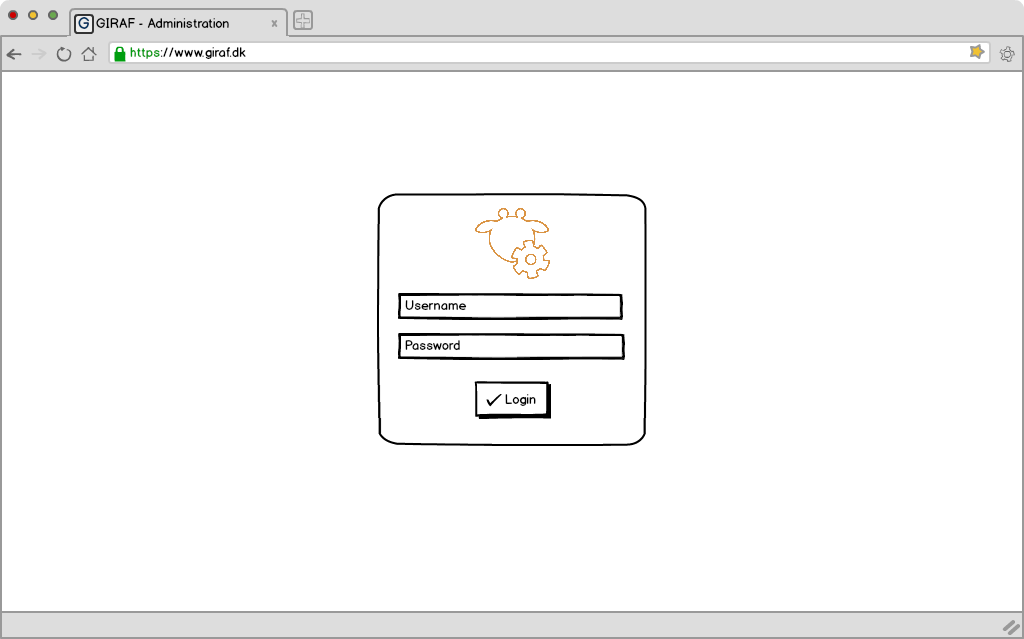
\includegraphics[width=1\textwidth]{images/mockup/login.png}
\caption{Login}
\label{fig:login}
\end{figure}

\newpage

\begin{figure}[!h]
\centering
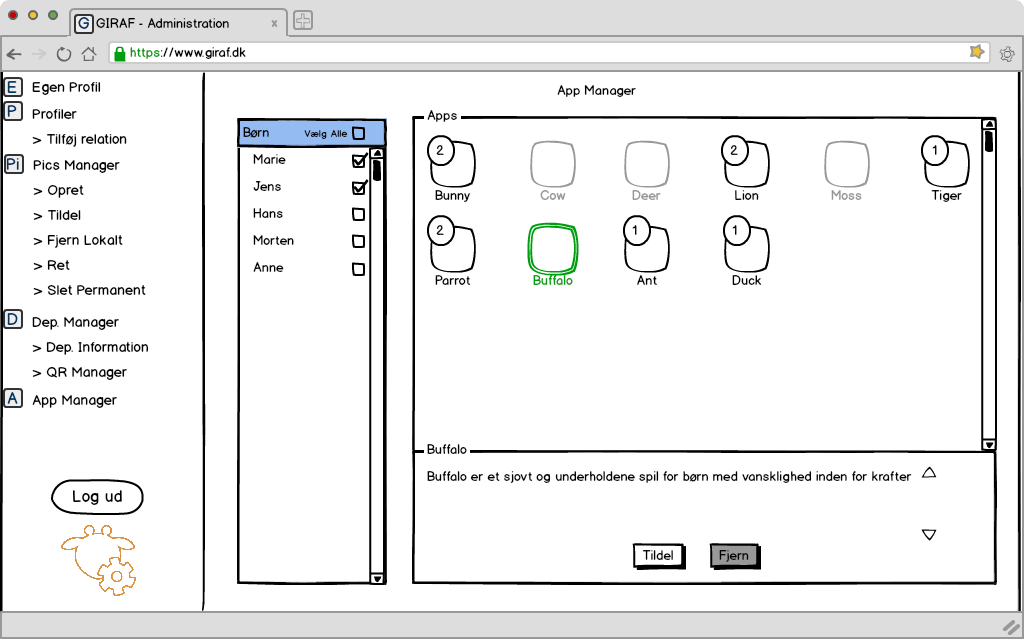
\includegraphics[width=1\textwidth]{images/mockup/app_manager.png}
\caption{App Manager}
\label{fig:app_manager}
\end{figure}

\begin{figure}[!h]
\centering
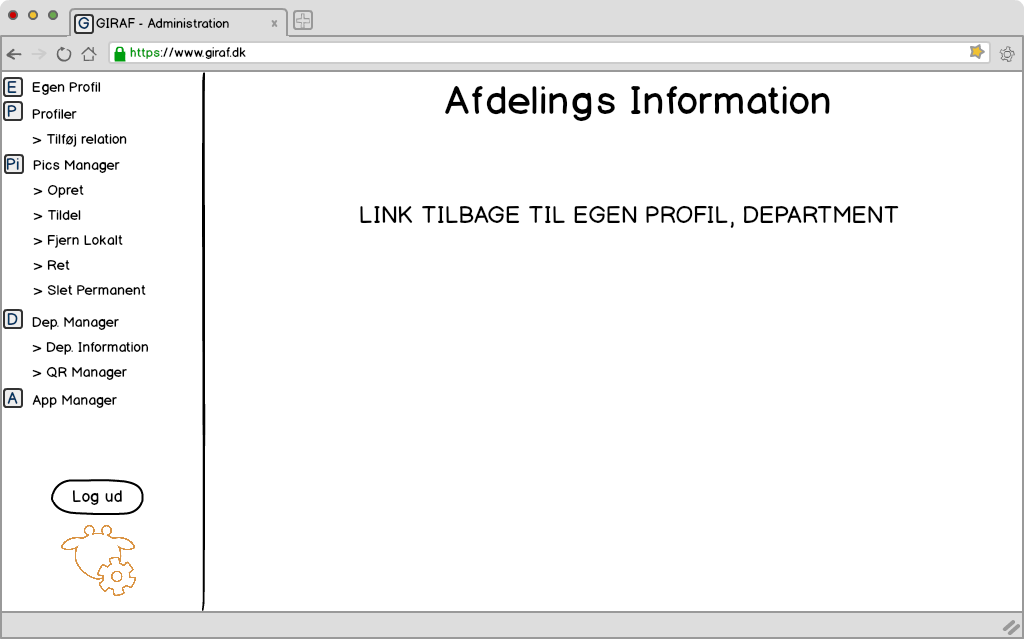
\includegraphics[width=1\textwidth]{images/mockup/deptInformation.png}
\caption{Department Information}
\label{fig:dept_information}
\end{figure}

\newpage

\begin{figure}[!h]
\centering
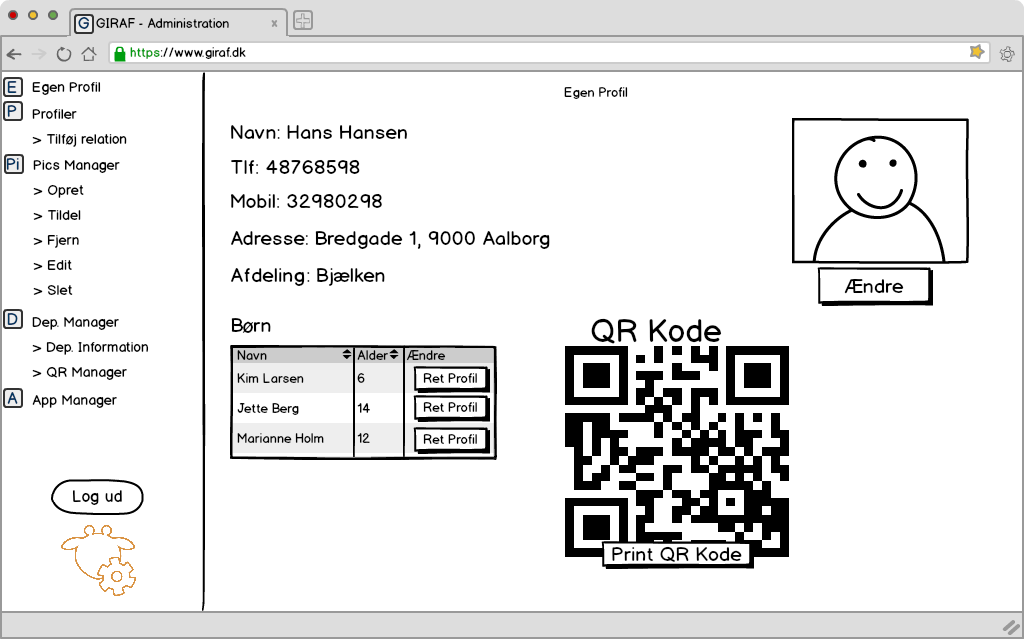
\includegraphics[width=1\textwidth]{images/mockup/egenProfil.png}
\caption{Own Profile}
\label{fig:own_profile}
\end{figure}

\begin{figure}[!h]
\centering
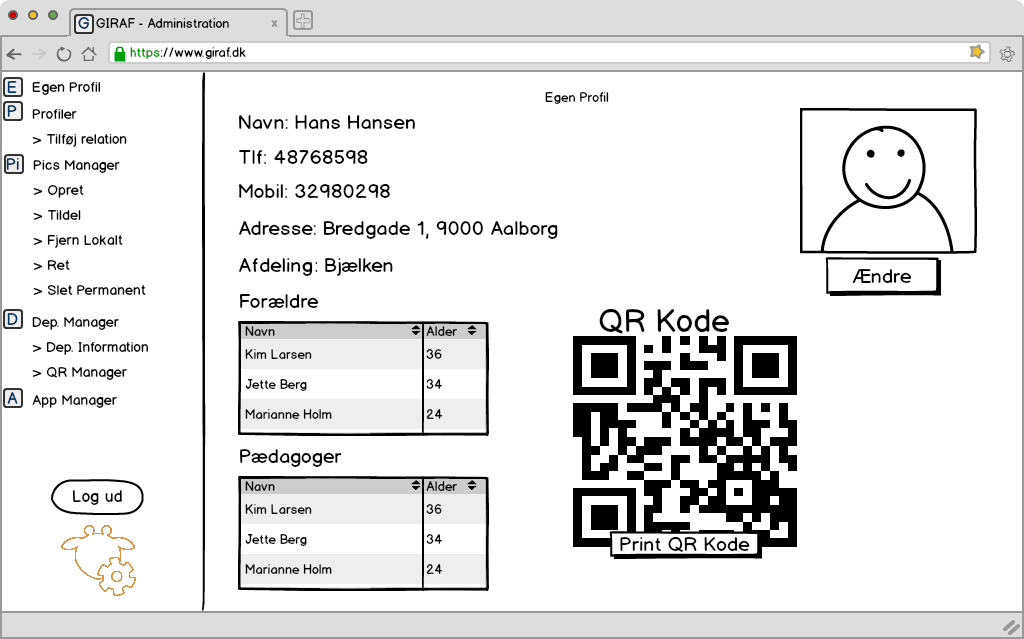
\includegraphics[width=1\textwidth]{images/mockup/egenProfilBarn.png}
\caption{Own Profile Child}
\label{fig:own_profile_child}
\end{figure}

\newpage

\begin{figure}[!h]
\centering
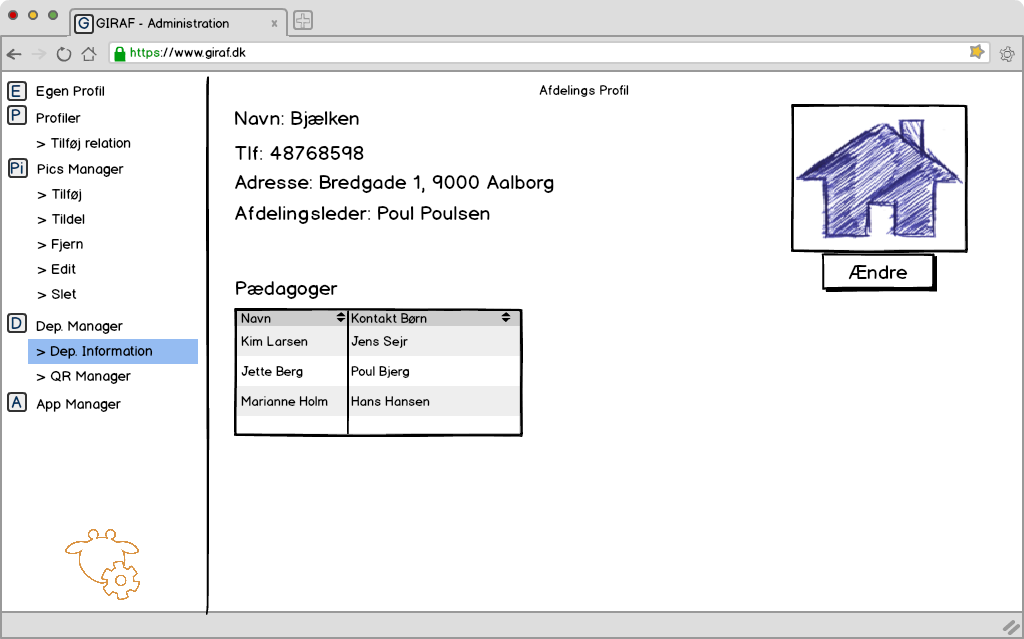
\includegraphics[width=1\textwidth]{images/mockup/egenProfilDepartment.png}
\caption{Own Profile Deparment}
\label{fig:own_profile_department}
\end{figure}

\begin{figure}[!h]
\centering
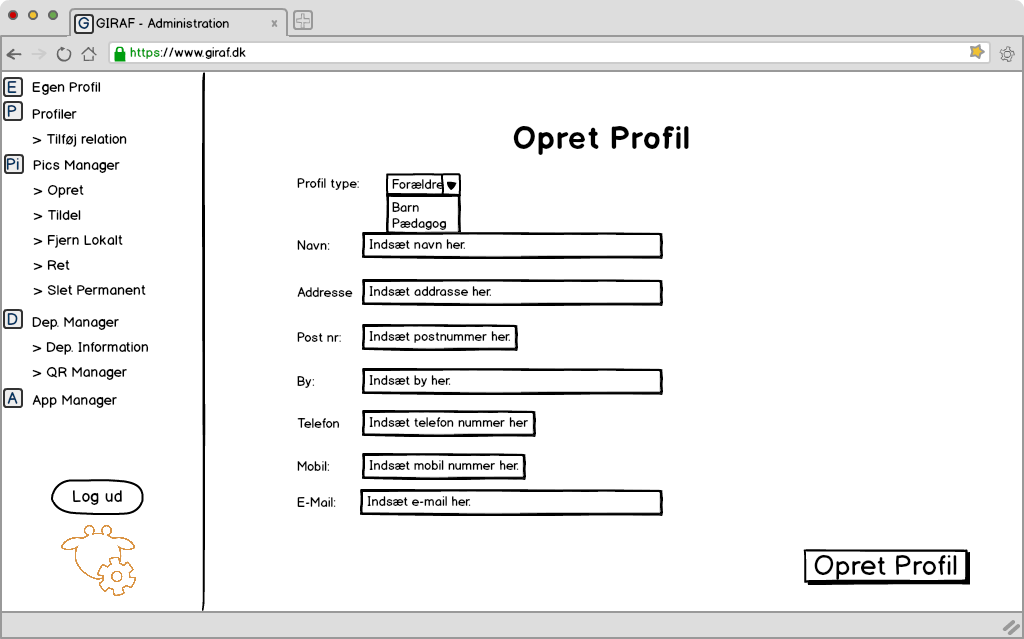
\includegraphics[width=1\textwidth]{images/mockup/egenProfilGaudiens.png}
\caption{Own Profile Guardian}
\label{fig:own_profile_guardian}
\end{figure}

\newpage

\begin{figure}[!h]
\centering
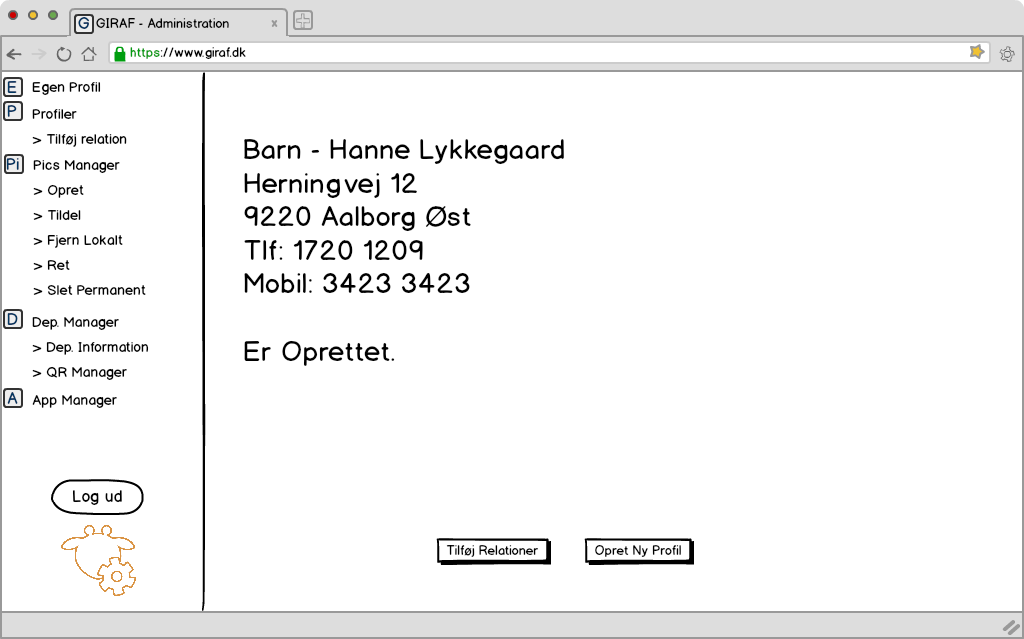
\includegraphics[width=1\textwidth]{images/mockup/opretProfilAccept.png}
\caption{Create Profile Accept}
\label{fig:create_profile_accept}
\end{figure}



\begin{figure}[!h]
\centering
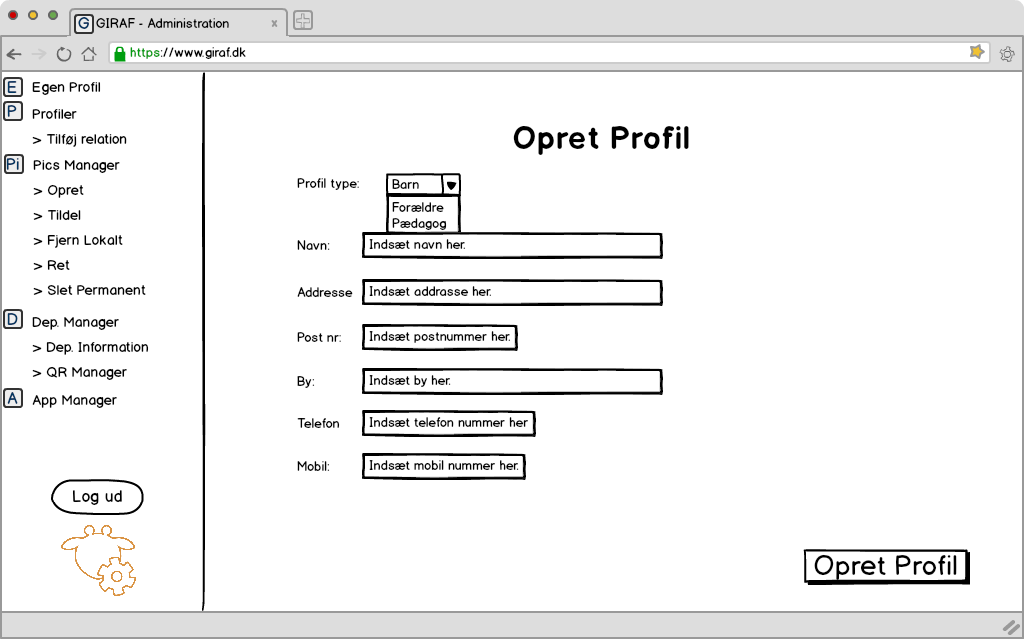
\includegraphics[width=1\textwidth]{images/mockup/opretProfilBarn.png}
\caption{Create Profile Child}
\label{fig:create_profile_child}
\end{figure}

\newpage

\begin{figure}[!h]
\centering
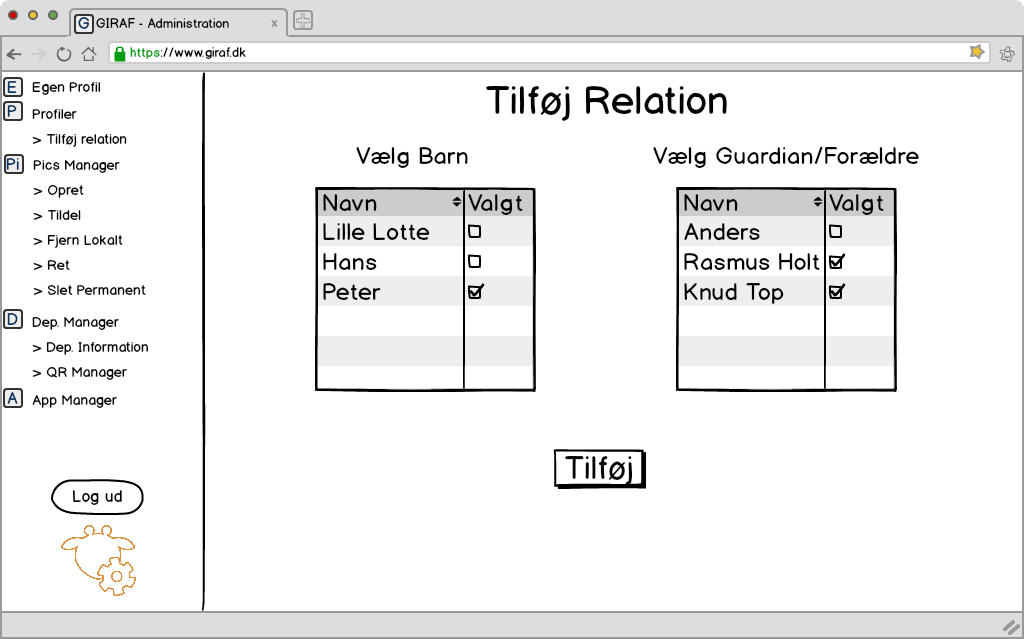
\includegraphics[width=1\textwidth]{images/mockup/opretRelation.png}
\caption{Create Relation}
\label{fig:create_relation}
\end{figure}

\begin{figure}[!h]
\centering
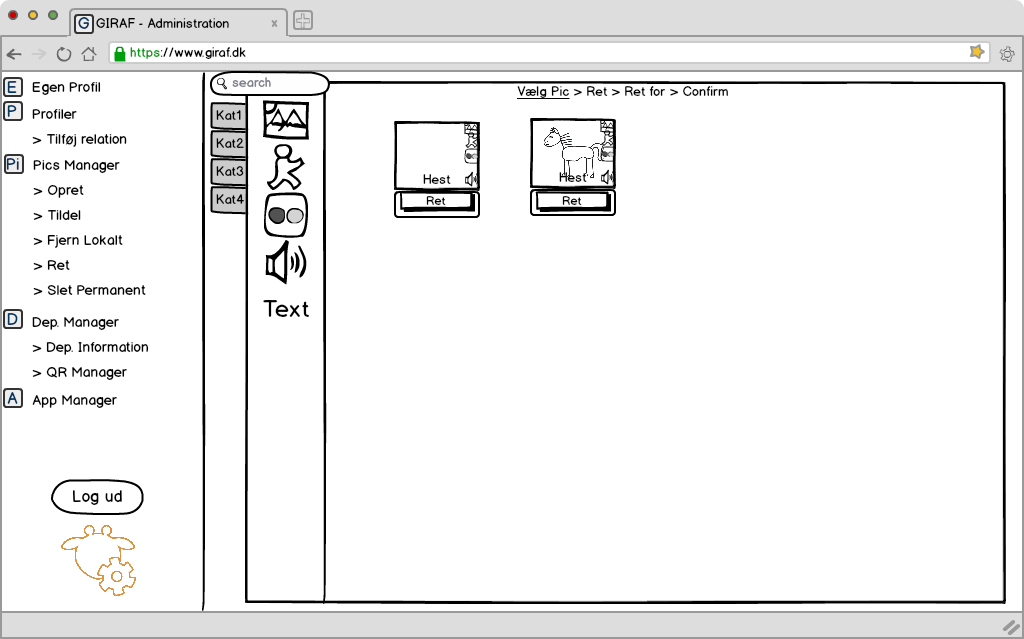
\includegraphics[width=1\textwidth]{images/mockup/picsManagerEdit.png}
\caption{Pics Manager Edit}
\label{fig:pics_manager_edit}
\end{figure}

\newpage

\begin{figure}[!h]
\centering
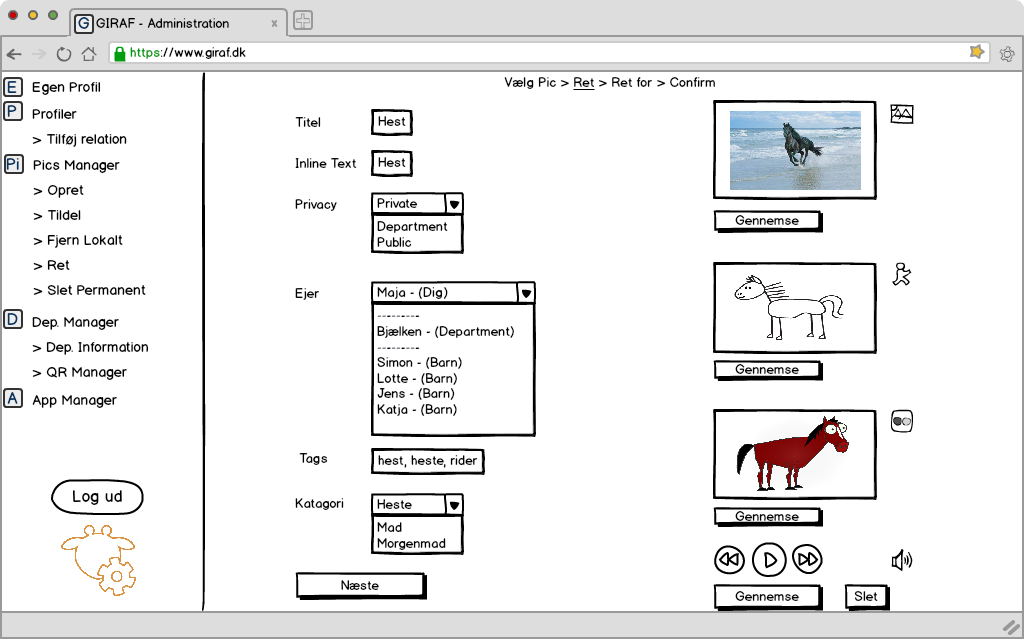
\includegraphics[width=1\textwidth]{images/mockup/picsManagerEdit2.png}
\caption{Pics Manager Edit 2}
\label{fig:pics_manager_edit2}
\end{figure}

\FloatBarrier

\begin{figure}[!h]
\centering
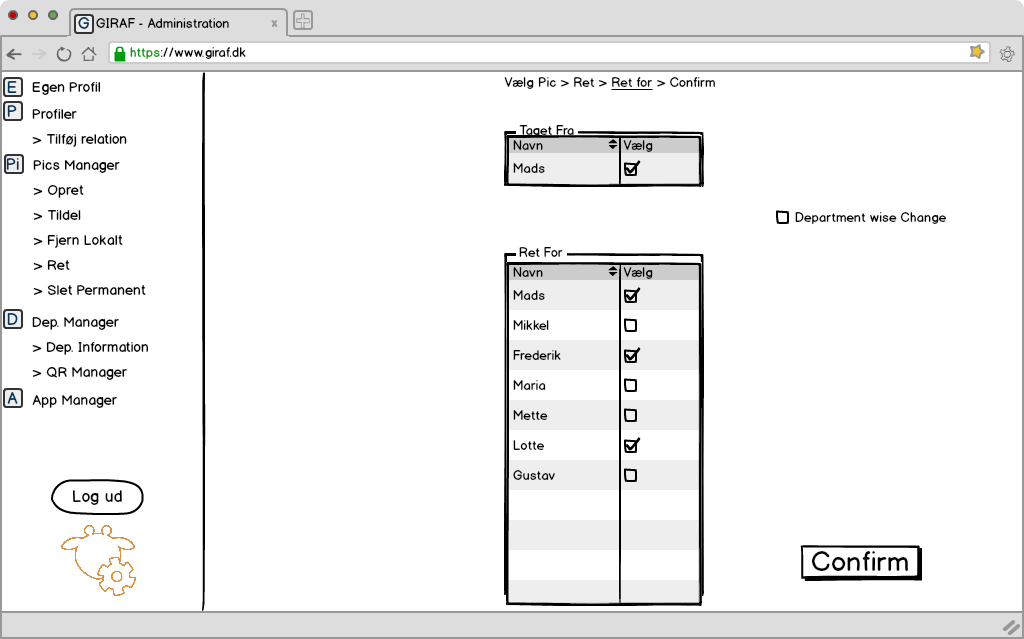
\includegraphics[width=1\textwidth]{images/mockup/picsManagerEdit3.png}
\caption{Pics Manager Edit 3}
\label{fig:pics_manager_edit3}
\end{figure}

\newpage

\begin{figure}[!h]
\centering
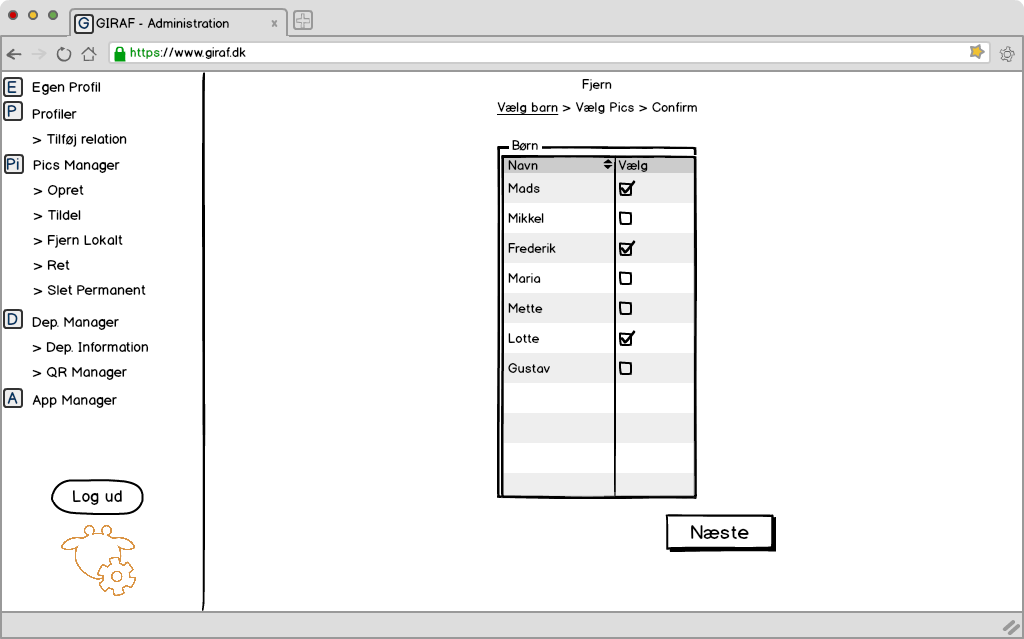
\includegraphics[width=1\textwidth]{images/mockup/picsManagerFjern.png}
\caption{Pics Manager Remove}
\label{fig:pics_manager_remove}
\end{figure}

\begin{figure}[!h]
\centering
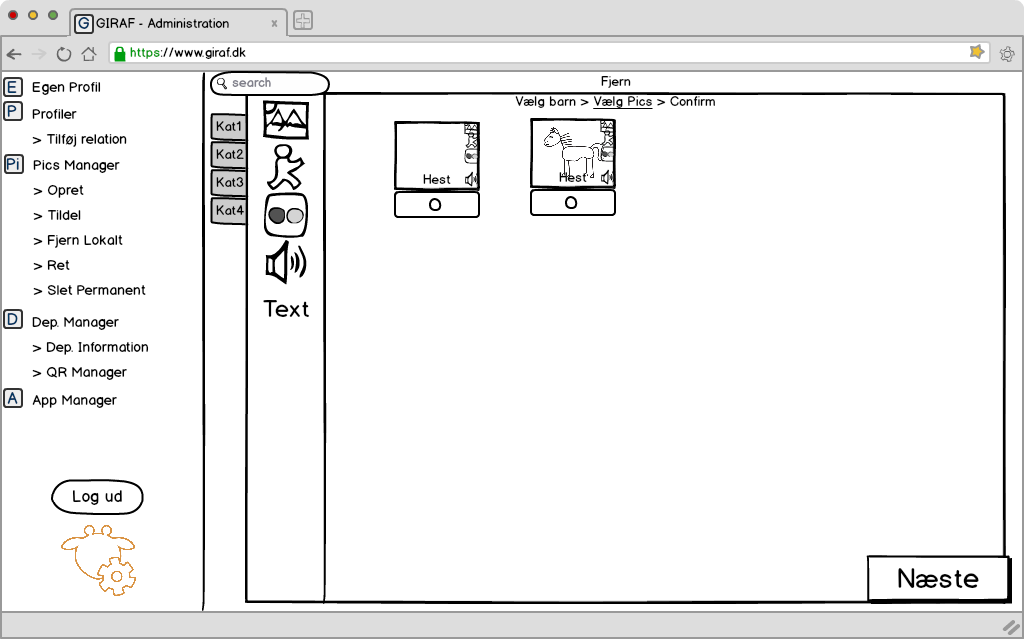
\includegraphics[width=1\textwidth]{images/mockup/picsManagerFjern2.png}
\caption{Pics Manager Remove 2}
\label{fig:pics_manager_remove2}
\end{figure}

\newpage

\begin{figure}[!h]
\centering
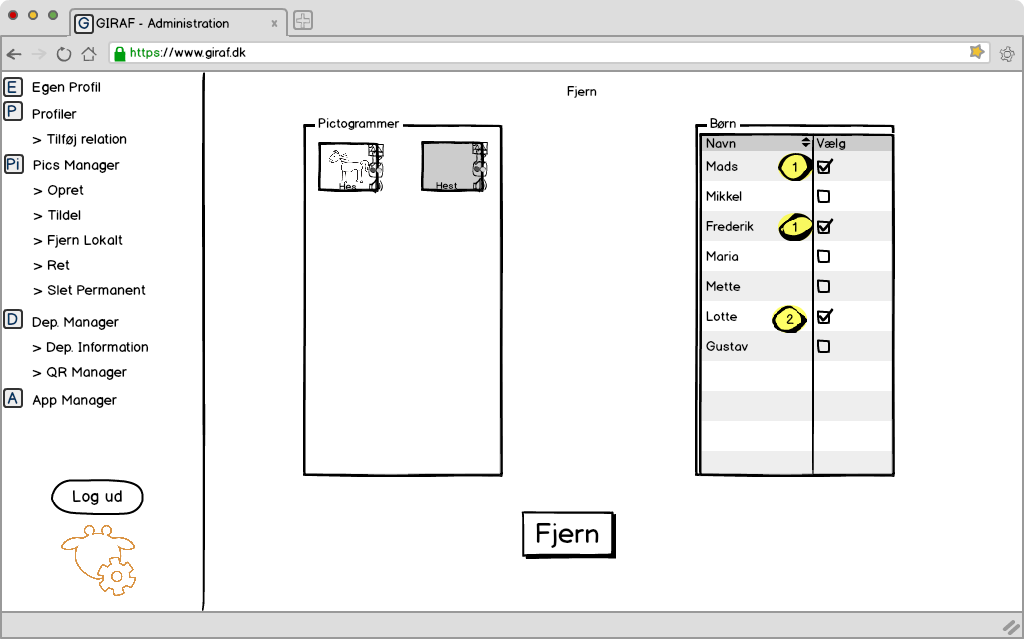
\includegraphics[width=1\textwidth]{images/mockup/picsManagerFjern3.png}
\caption{Pics Manager Remove 3}
\label{fig:pics_manager_remove3}
\end{figure}

\begin{figure}[!h]
\centering
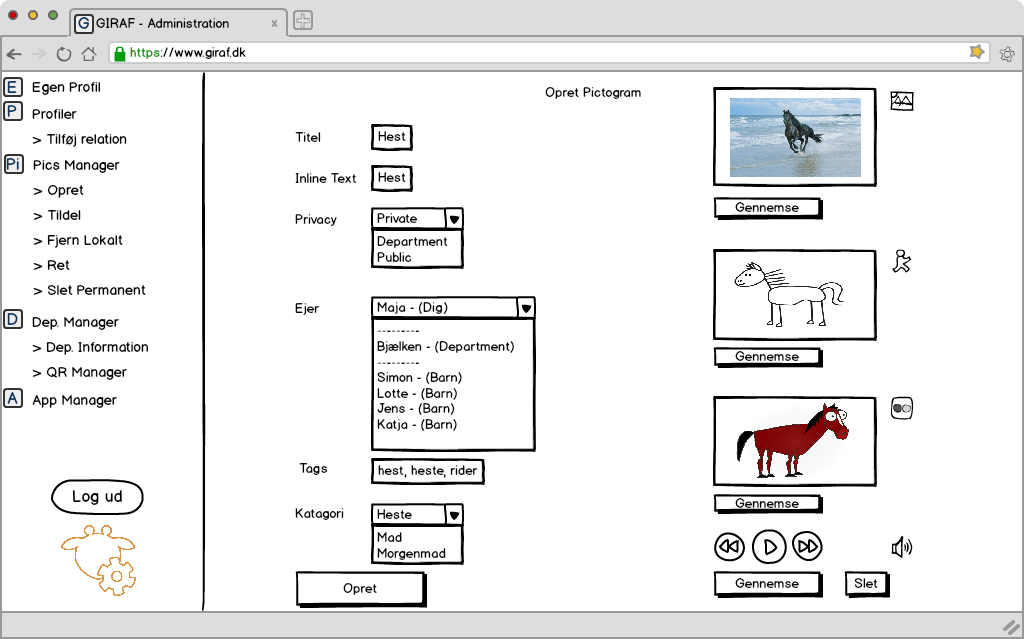
\includegraphics[width=1\textwidth]{images/mockup/picsManagerOpret.png}
\caption{Pics Manager Create}
\label{fig:pics_manager_create}
\end{figure}

\newpage

\begin{figure}[!h]
\centering
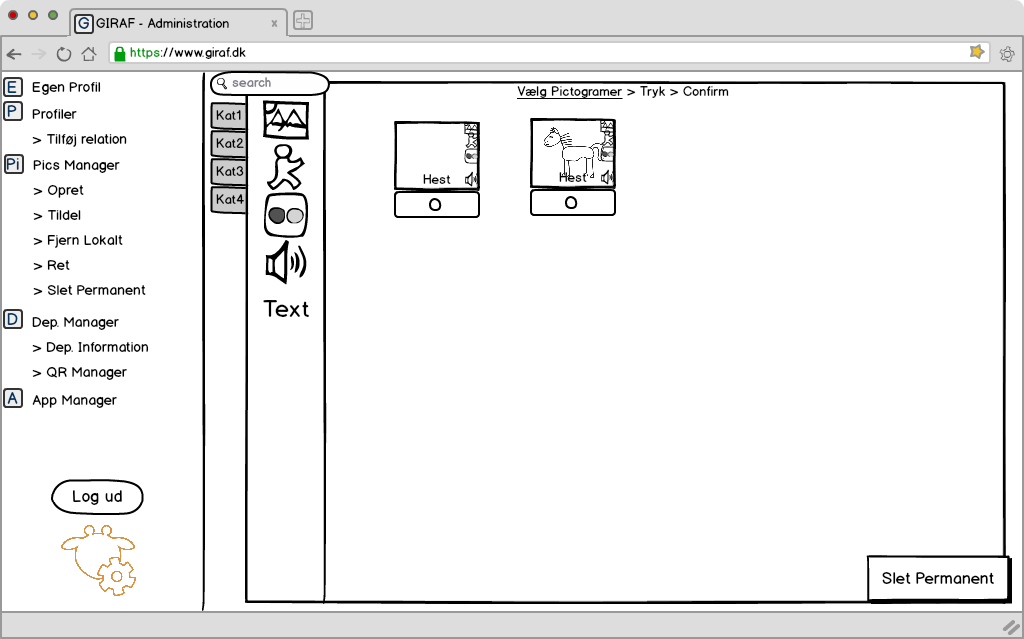
\includegraphics[width=1\textwidth]{images/mockup/picsManagerSlet.png}
\caption{Pics Manager Delete}
\label{fig:pics_manager_delete}
\end{figure}

\begin{figure}[!h]
\centering
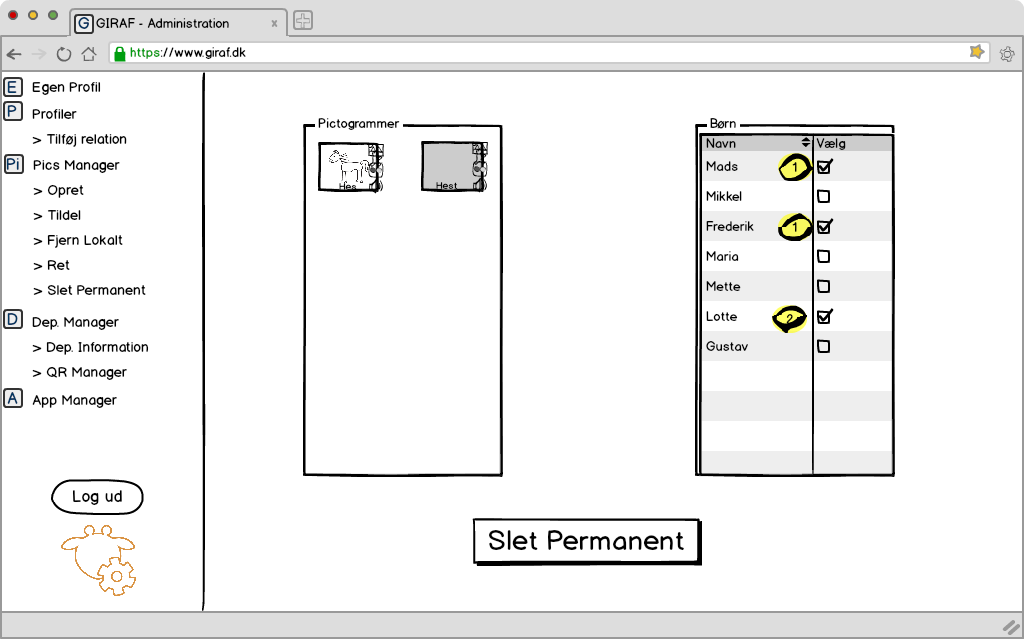
\includegraphics[width=1\textwidth]{images/mockup/picsManagerSlet2.png}
\caption{Pics Manager Delete 2}
\label{fig:pics_manager_delete2}
\end{figure}

\newpage

\begin{figure}[!h]
\centering
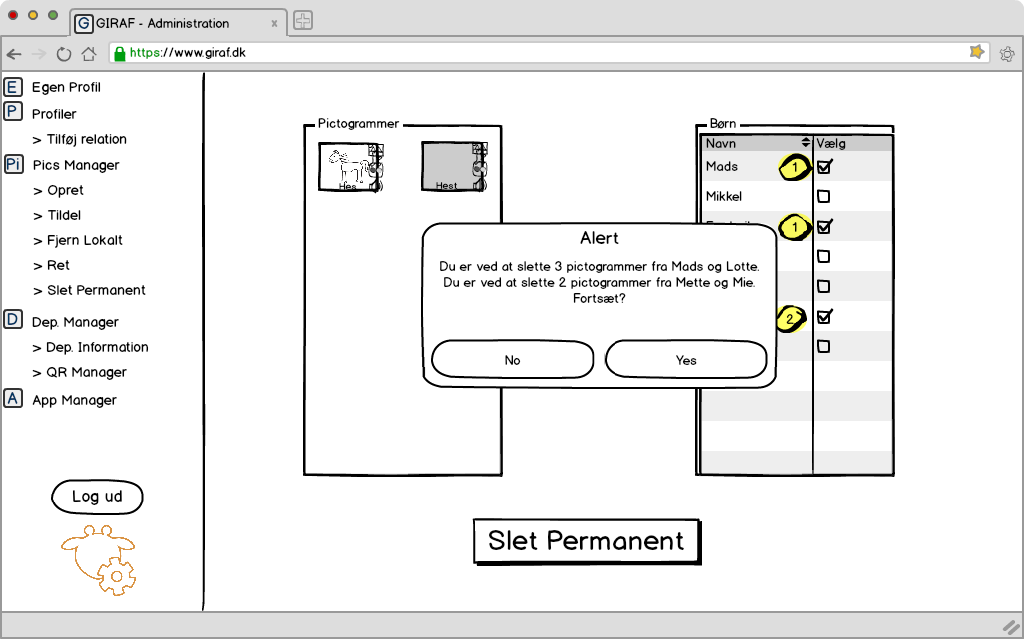
\includegraphics[width=1\textwidth]{images/mockup/picsManagerSlet3.png}
\caption{Pics Manager Delete 3}
\label{fig:pics_manager_delete3}
\end{figure}

\begin{figure}[!h]
\centering
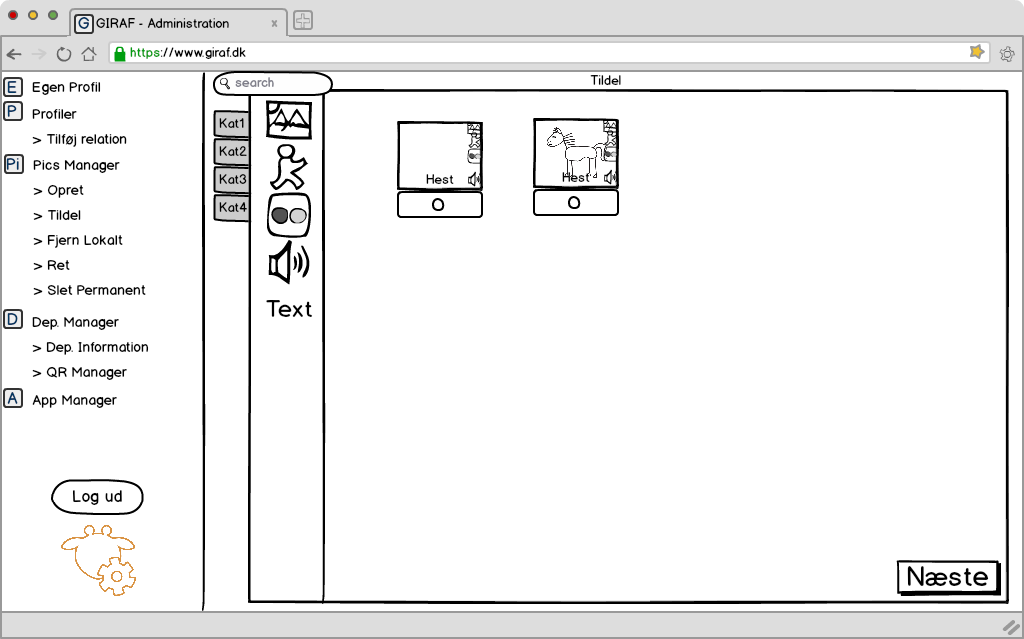
\includegraphics[width=1\textwidth]{images/mockup/picsManagerTildel.png}
\caption{Pics Manager Assign}
\label{fig:pics_manager_assign}
\end{figure}

\newpage

\begin{figure}[!h]
\centering
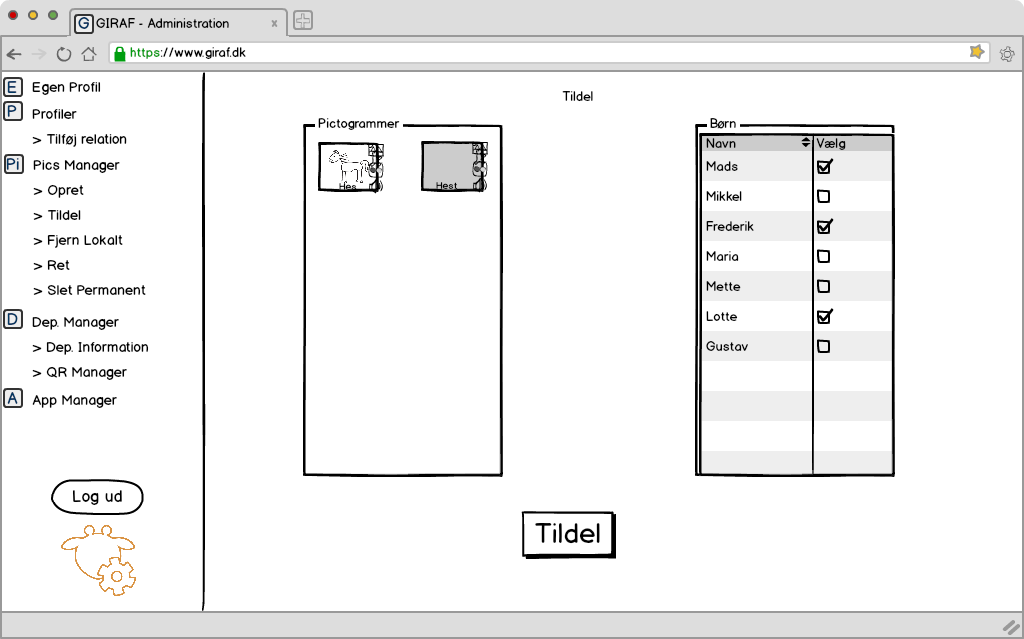
\includegraphics[width=1\textwidth]{images/mockup/picsManagerTildel2.png}
\caption{Pics Manager Assign}
\label{fig:pics_manager_assign2}
\end{figure}

\begin{figure}[!h]
\centering
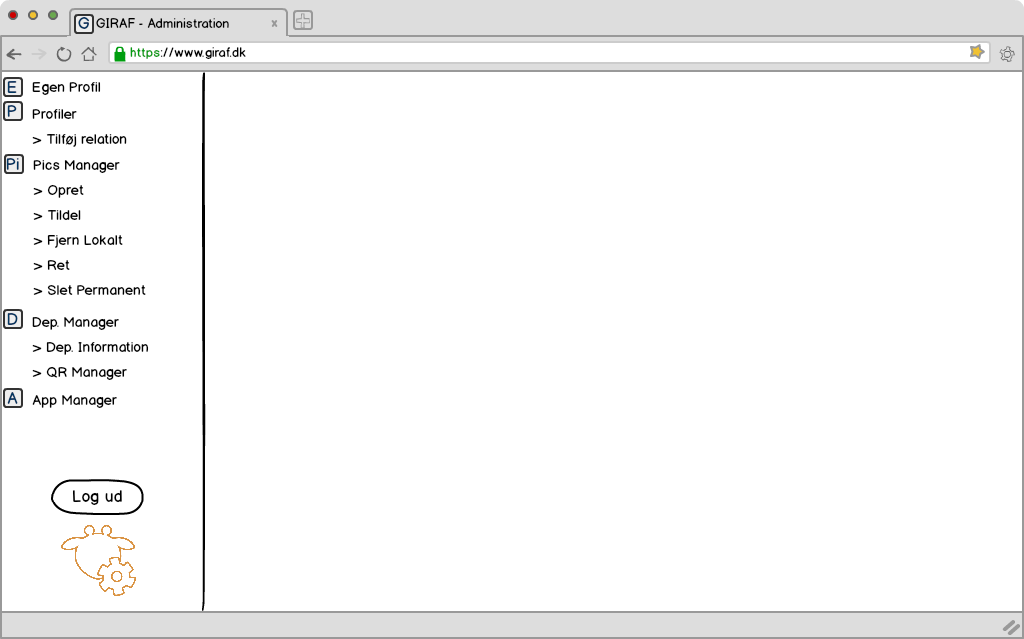
\includegraphics[width=1\textwidth]{images/mockup/profiler.png}
\caption{Profiles}
\label{fig:profiles}
\end{figure}

\newpage

\begin{figure}[!h]
\centering
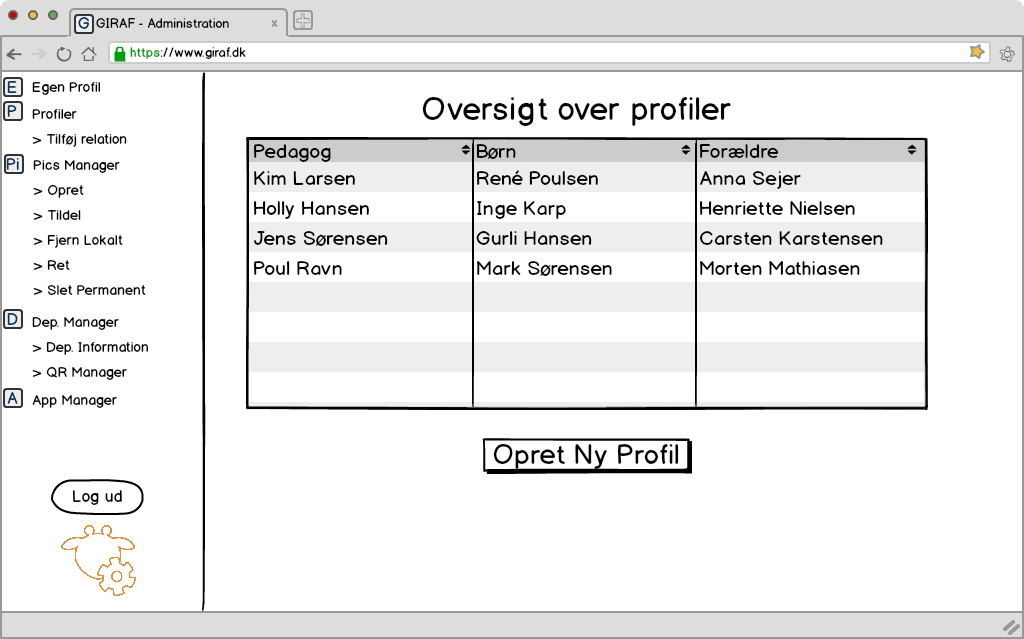
\includegraphics[width=1\textwidth]{images/mockup/profilerDeptManager.png}
\caption{Profiles Department Manager}
\label{fig:profiles_dept_manager}
\end{figure}

\begin{figure}[!h]
\centering
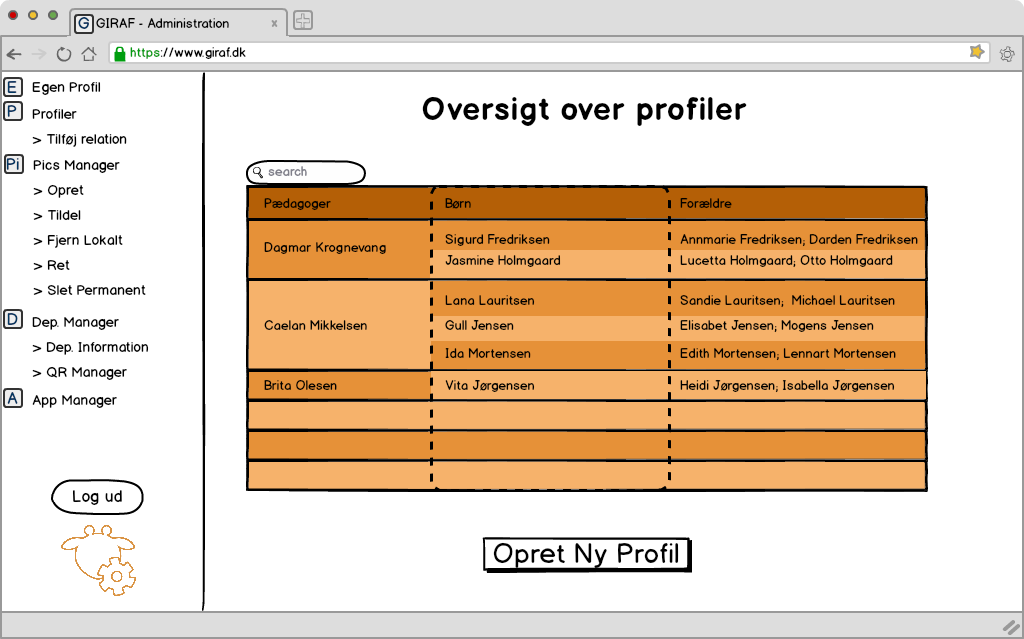
\includegraphics[width=1\textwidth]{images/mockup/profilerDeptManager1.png}
\caption{Profiles Department Manager 2}
\label{fig:profiles_dept_manager2}
\end{figure}

\newpage

\begin{figure}[!h]
\centering
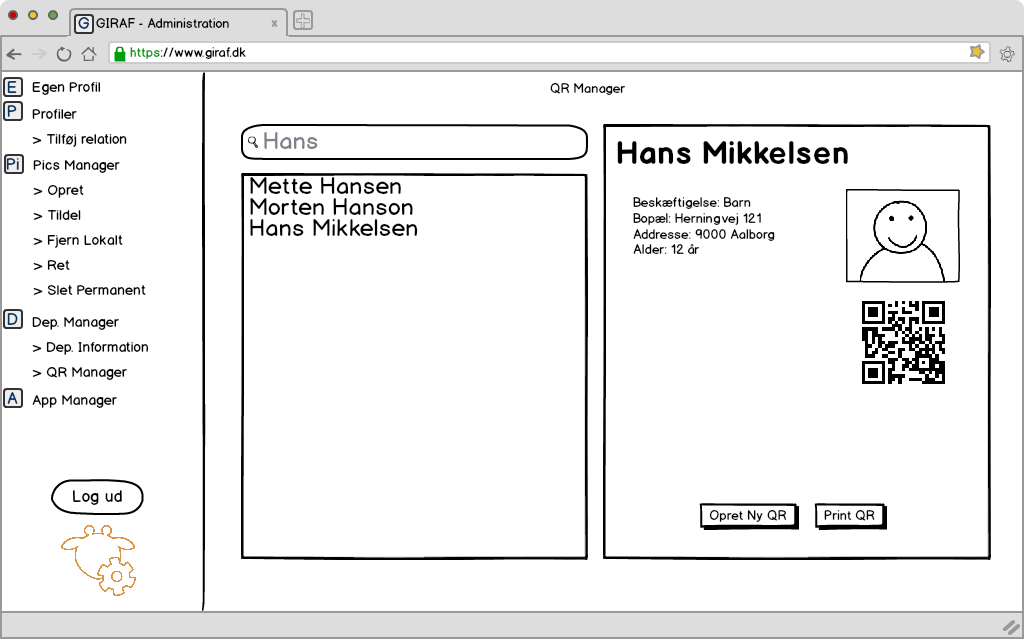
\includegraphics[width=1\textwidth]{images/mockup/QR_manager.png}
\caption{QR Manager}
\label{fig:qr_manager}
\end{figure}

\begin{figure}[!h]
\centering
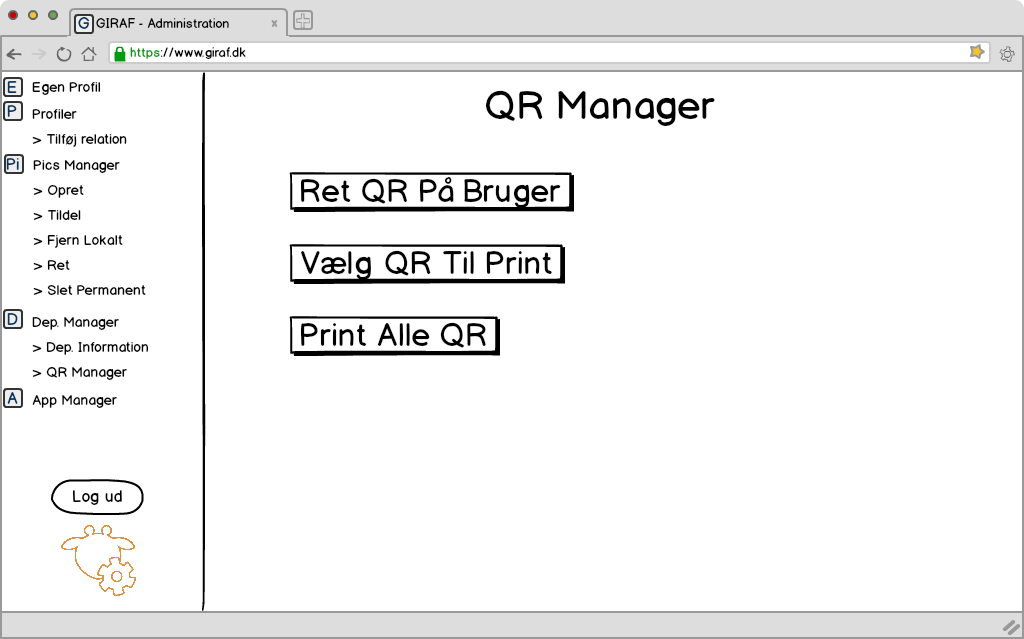
\includegraphics[width=1\textwidth]{images/mockup/qrManagerFront.png}
\caption{QR Manager Frontpage}
\label{fig:qr_manager_front}
\end{figure}

\newpage

\begin{figure}[!h]
\centering
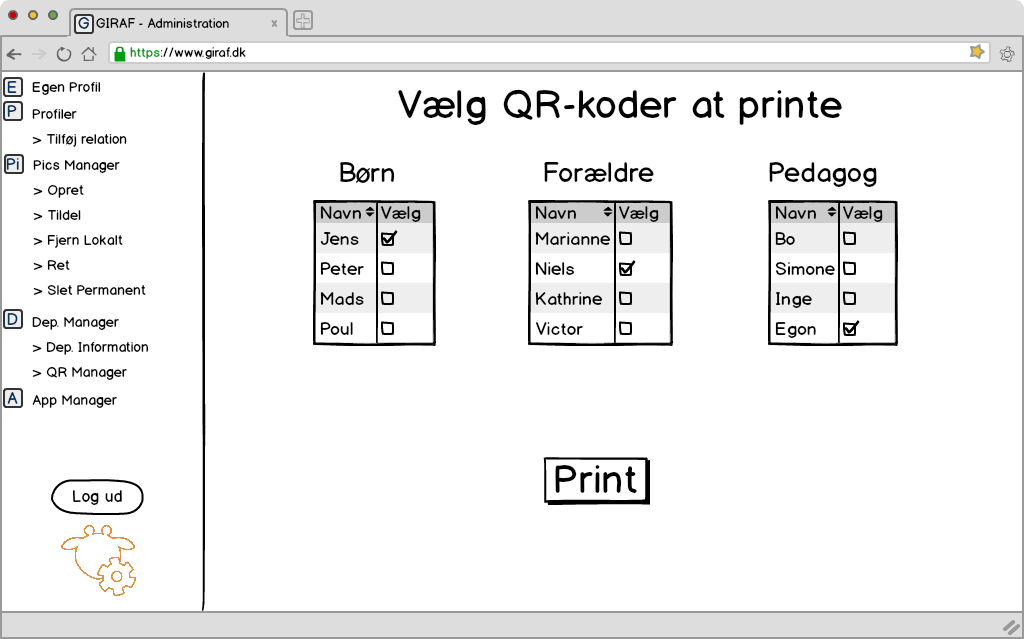
\includegraphics[width=1\textwidth]{images/mockup/qrManagerPick.png}
\caption{QR Manager Pick}
\label{fig:qr_manager_pick}
\end{figure}

\begin{figure}[!h]
\centering
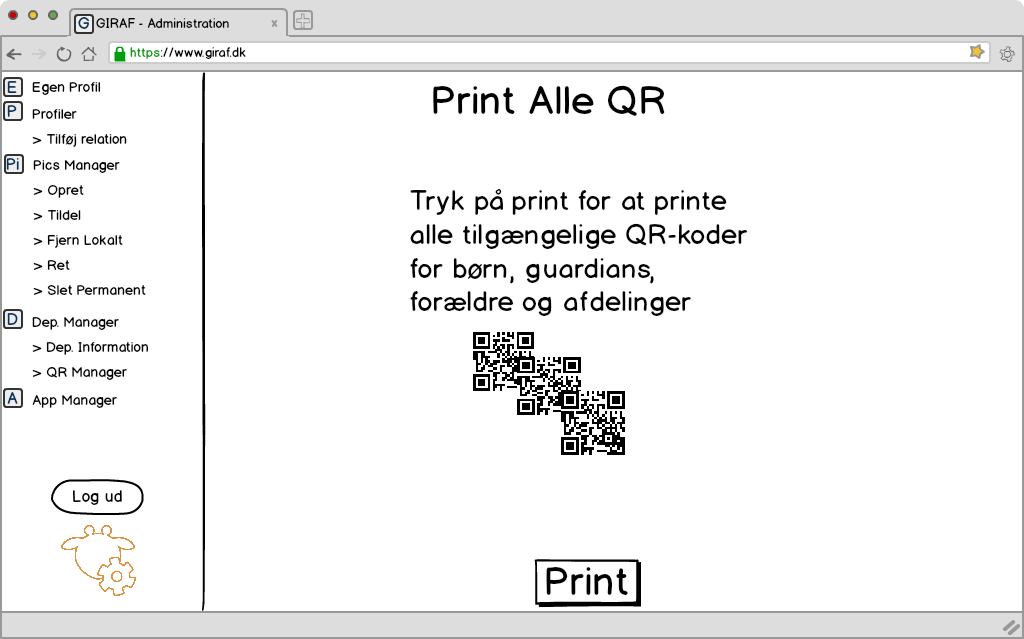
\includegraphics[width=1\textwidth]{images/mockup/qrManagerPrintAll.png}
\caption{QR Manager Print All}
\label{fig:qr_manager_print_all}
\end{figure}
	\chapter{Transcript of Meeting with the head of the kindergarten (1/3-2013)}
\label{interviewMette}

\textbf{The questions we brought with us:}\\
A: Does the parents have a common contact list between each other, like the ones used in the, Danish, elementary school?\\
B: How often do you change the kids pictograms? - As in all the way out of the scrap book\\
C: How many kids does a pedagogue take care of, on average?\\
D: How is the parents allowed to influence the daily life of their kids, when the kids are at the kinder garden?\\
E: Does the department manager have a list of the e-mails of each parent and are they easy to find? - If not, how easy would it be to gather them?\\
\\
\textbf{Answers to these questions:}\\
A: The parents are not allowed to know anything about each other or the other parents kids.\\
\\
B: It doesn’t happen that often, but they still need to be able to change the pictures really fast. Since sometimes the kids come in with a new jacket, and cannot put their jacket back on, or take it off because of the wrong visual stimuli from an old picture.\\
The same goes if the milk carton suddenly changes to a Christmas theme or such.\\
\\
C: A pedagogue usually have the responsibility for 2-3 kids. - These are called ''kontakt børn''.\\
\\
D: The parents have no influence. Actually if their kids cannot participate in outdoor activities because of illness or tiredness, the parents are told to keep their kids at home if the plan for the day involves outdoor activity, (which they at Bækken do almost every day).\\
\\
E: She has their e-mail, but they are not public accessible. This still makes it possible for her to send invites to the system. - We were informed that the registration forms for when a kid enters the kinder garden has been updated so that the parents are asked to fill in their e-mail address.\\
\\
\textbf{Information gathered for PictoCreater group:}\\
- The text should not be stationary.\\
- There should be an option for drawing lines and removing parts of a pictogram.\\
These two lines were derived from what she told us of their current pictogram editor system.\\
\\
\textbf{Possible future work:}\\
1. A planning tool. The department manager uses a certain amount of time on scheduling the kids and pedagogues day. One of the most serious issues could be that one of her pedagogue had to take the day off, then she must make sure that all her schedules get taken care of. A feature that they could really use would be that of fixing an assignment for each second week.\\
This planning tool should also be able to print two different versions of the schedule. One for the parents and one for the pedagogues. - The parents are not supposed to know which kids do what, or with whom. They only need to know what general activities is taking place in the kindergarten.\\
She also suggested that the taxa schedule could be incorporated in this system.\\
\\
\textbf{Other observations:}\\
''Profiler'' - We noticed that the tab ''Profiler'' from our original design was of no use to anyone but the department manager. Since everyone else only had access to a certain list of persons, that we already displayed on ''Egen Profil''.\\
\\
''Profiler'' - Should be ordered in a table, where first the pedagogues name is, the next <td> should then contain the kids they are responsible for, the next <td> should then contain the parents of this kid, and the last <td> should then contain other relevant persons or information about the kid. (<td> is the same as a cell in a table)\\
\\
''Parent/Pedagogue contact'' - They don't communicate all that much in person. Since a department can have kids from basically all over the country. The kindergarten do host some 'parent, come and see the kindergarten nights'. But outside that they only communicate via phone and this black book the kids bring to and from the kindergarten. In it important information like, if the kid did something special today, or the reason why he arrived home with a new pair of pants on, and so forth. - The pedagogues always check this book when the kid arrives and so does the parents.\\
\\
''Privacy setting'' - The privacy setting private is known as ''mine tavler'' by the pedagogues.\\
\\
''Privacy setting'' - We need 5 different privacy settings: \\
Pedagogues only\\
Parents only\\
Guardians (''værger'') - We need to confirm this phrasing with the head of the kindergarten\\
Department\\
Public\\
\\
''Searching'' - When searching through tags or categories, it should search on synonyms as well.\\
\\
''Breadcrumbs'' - There should be breadcrumbs on every screen, or if there is only one action on the screen, it should contain its title.\\
\\
''Pictogram 'Edit' and 'Opret''' - We forgot to add category and tag adding to these functions.\\
\\
''App Manager'' - She found it intuitive to perform special settings on the apps in the app manager. - This could be an interesting design idea, but hard to implement.












	\chapter{Usability Testing Appendix}
\label{usabilityTestingAppendix}
This chapter contains the introduction given to the test persons and the tasks they had to perform. This chapter is written in danish, as was the test.\\
\\
\textbf{Opgaver:}\\

\begin{itemize}
	\item Ændre egen profils information, her i blandt: Navn, mail, tlf., profil billede
	\item	Opret nyt barn
	\item	Opret barns forældre
	\item	Opret pædagog
	\item	Opret relation mellem forældre og barn
	\item	Opret relation mellem pædagog og barn
	\item	Ret information om afdeling
	\item	Opret pictogram
	\item	Opret kategori
\end{itemize}

\textbf{Første Login:}\\
Du har nu fået en helt ny bruger i Giraf systemet, og opdager at dit navn er stavet forkert og der mangler tlf. nummer og et profil billede.\\
Vi vil derfor bede dig om at opdatere følgende: Dit navn, dit tlf. nummer og uploade dit profil billede.\\
Vi har lagt et billede på skrivebordet med navnet ''profilBilledePige.jpg'' og ''profilBilledeDreng.jpg''\\
\\
\textbf{Nyt barn i afdelingen:}\\
I morgen starter det nye barn, Thorsten Jensen, i afdelingen og han har derfor brug for at få oprettet en profil. Hans forældre hedder Lotte og Mads Jensen. For at Lotte og Mads også skal have mulighed for at benytte systemet derhjemme skal de også oprettes i systemet.\\
Lottes e-mail: lotte.jensen@test.dk\\
Mads’ e-mail: mads.jensen@test.dk\\
Vi vil bede dig om at oprette en profil til Thorsten, Lotte og Mads.\\
\\
\textbf{Hvems forældre er det?}\\
Nu har Thorsten, Lotte og Mads fået oprette en profil. Men før at Lotte og Mads kan bruge deres profiler til noget skal de forbindes med Thorsten.\\
Vi vil derfor bede dig oprette en forbindelse mellem Thorsten og Lotte, samt en forbindelse mellem Thorsten og Mads.\\
\\
\textbf{Den nye Pædagog:}\\
I dag starter den nye pædagog Henriette Poulsen også i afdelingen, hun skal have ansvaret for Thorsten.\\
Henriette Poulsens informationer:\\
E-mail: henriette.poulsen@test.dk\\
Tlf: 88 44 55 66\\
Add.: Mark Poulsen Vej 23 – Aalborg Øst 9220\\
Vi vil derfor bede dig om at oprette en profil til Henriette og dernæst oprette en relation mellem Henriette og Thorsten.\\
\\
\textbf{Ny Tlf. i afdelingen}\\
I har fået besked ovenfra på at skifte jeres telefon nummer i afdelingen. I har i dag modtaget det nye telefon nummer.\\
Det nye nummer er: 87 78 23 44\\
Vi vil nu bede dig om at rette informationen om jeres afdeling så den passer.\\
\\
\textbf{Pictogram af de nye shorts:}\\
Thorsten har lige fået nye shorts og I er blevet tilsendt et billede af Thorsten hvor han er iført sine nye shorts.\\
I vælger for at være på forkant med Thorstens pictogram kartotek at oprette et pictogram af hans shorts.\\
Vi vil derfor nu bede dig om at oprette et pictogram som hedder Shorts.\\
Billedet til pictogrammet kan findes på skrivebordet: ''shorts.jpg''\\
\\
\\
\textbf{Introduktion:}\\
Velkommen til testning af GIRAF admin systemet.\\
Vi vil stille dig en række opgaver, skrevet ned på papir, som vi gerne så dig udfører på den fremstillede PC. Testens formål er for os at drage indsigt i din måde at arbejde på, vi vil derfor bede dig tænke højt imens du udfører opgaverne. – Vi vil her gøre opmærksom på at intet er for småt til at vi gerne vil hører det.\\
Igennem testen vil <navn> sidde med dig i testrummet mens du udfører opgaverne. Hvis du har spørgsmål til opgaverne vil <navn> hjælpe dig. Han vil også give dig den næste opgave når du har gennemført den du var i gang med.\\
Vi optager testprocessen på film og har derfor brug for at du skriver under på at dette er okay. <Udlever underskrifts side og giv tid til at underskrive>

	\chapter{Colour Theme}
\label{chap:colorTheme}
\vspace{-5mm}
\begin{figure}[!h]
\centering
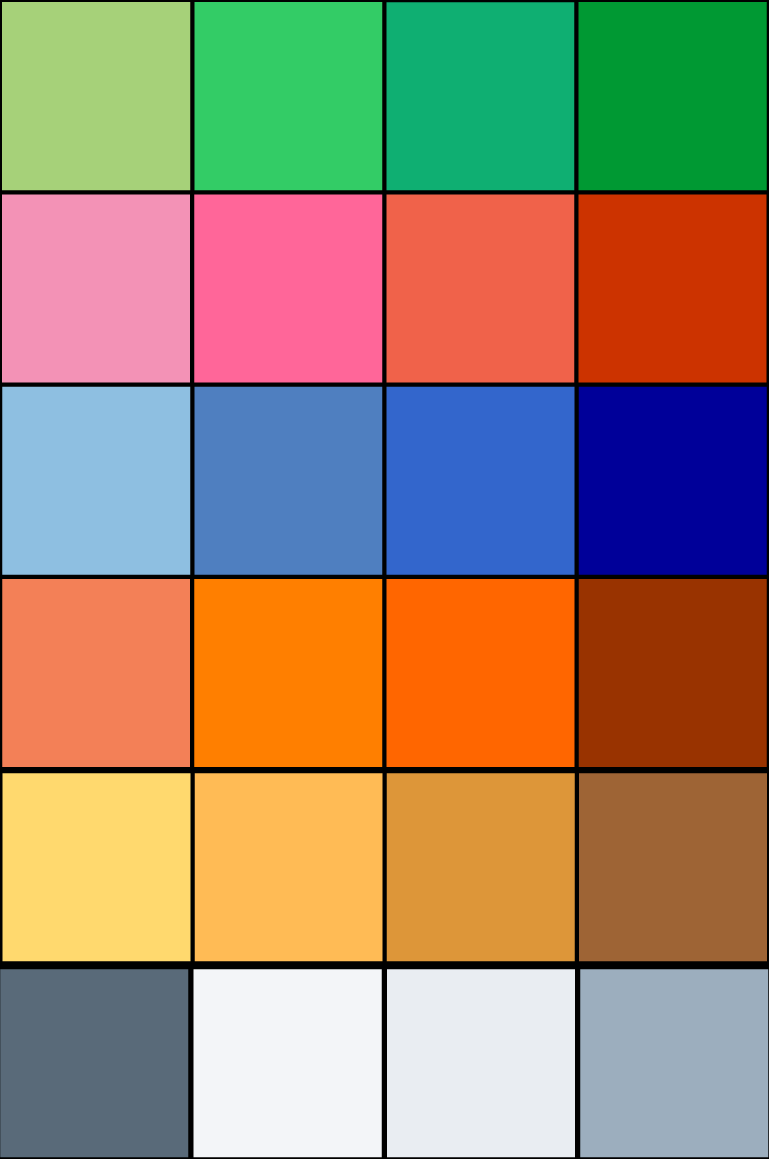
\includegraphics[width=0.6\textwidth]{images/colorTheme.png}
\caption{Colour theme for the \ac{giraf} system.}
\end{figure}

	\end{appendices}
	
	%Denne komando lister alle fixme's
	%\part{Fixme}
	%\listoffixmes

\end{document}
